\documentclass[11pt]{article}
\usepackage[textheight=9in]{geometry}
\usepackage{graphicx}
\usepackage{epstopdf}
\usepackage{listings}
\usepackage{float}
\usepackage{csvsimple}
\usepackage{wrapfig}
\usepackage{longtable}

\begin{document}
\section{1/24/16}
\subsection{Permutation testing}
In order to test how the algorithm returns the permutation results, I set up sample matrices using \verb|create_toy.m| and recorded the distance between the result returned by the algorithm (\verb|eig_perm|) and that of the actual input data (\verb|ss|).

\lstset{language=Matlab, caption=Compare Permutations}
\begin{lstlisting}[frame=single]
rois = 33;
noise_mag = 0;
trace_type = 'sines';
shift = 10;
y = zeros(1,100);
for i = 1:length(y)
	[Z, ss] = create_toy(trace_type, 'rois', rois, ...
		'noisemag', noise_mag, ...
		'shift', shift);
	[eig_phases,eig_perm,slm,evals] = cyclic_analysis(Z);
	y(i) = cyclic_distance(ss,eig_perm);
end
plot(y)
\end{lstlisting}

The function \verb|create_toy| produces a set of \verb|rois| identical sine waves randomly spread over a \verb|shift| time step period (i.e., each copy of the trace is shifted along the x axis so that all copies are within \verb|shift| time steps of each other). The variable \verb|ss| shows the ordering of the traces produced. Using the setting above, for example, a data set like that in on the left of Figure 1 is produced. The figure on the right shows that the algorithm returns the identical permutation each time.
\begin{figure}
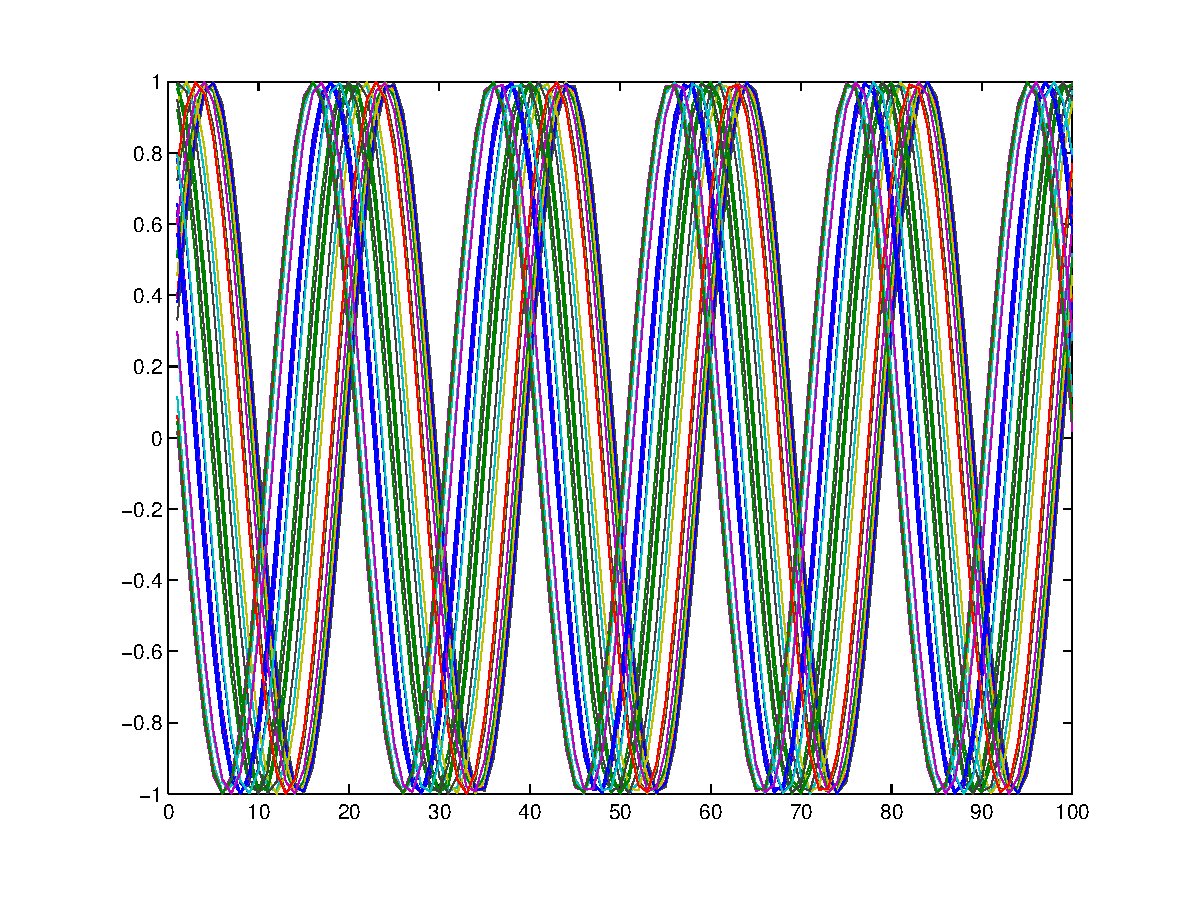
\includegraphics[width=.45\textwidth]{pictures/1_24_16/sine_toy.eps}
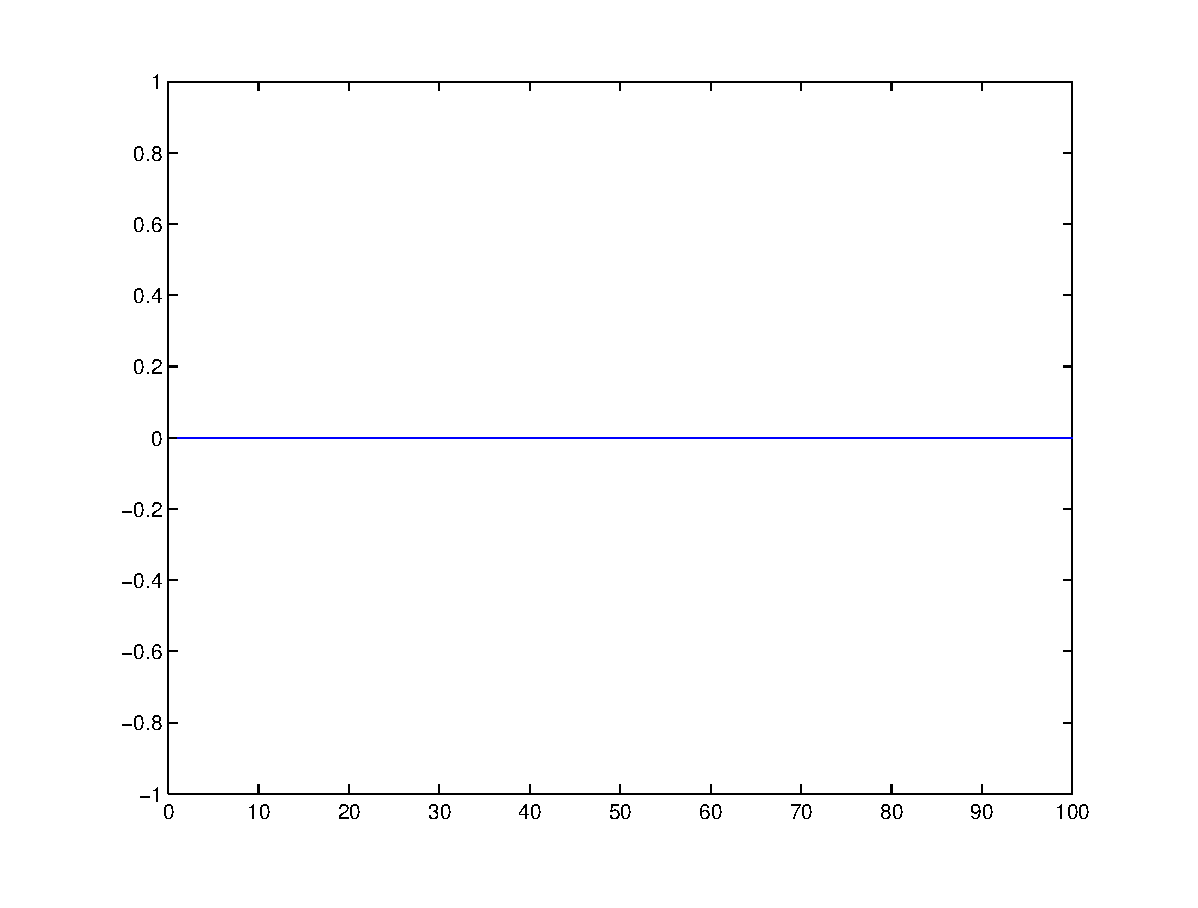
\includegraphics[width=.45\textwidth]{pictures/1_24_16/sine_cpsn_noNoise.eps}
\caption{Left: Sample data created from sine waves shifted randomly at most 10 time steps apart (no added noise). Right: Comparison of the permutation returned by the algorithm with that of the actual data set for 100 separately generated data sets.}
\end{figure}
The distance is measured using \verb|cyclic_distance(V1,V2)| which simply counts the how many steps V2 is from V1 (let V1 be (1:5), then [2,1,3,4,5] is a distance of 1 from V1 and [2,3,4,5,1] is a distance of 5 from V1.) This doesn't really count "cyclic distance" but works for this application since we would like to see if we are picking up the correct starting point and cycling in the right direction. 
Increasing \verb|shift| to 18 (the period for the sine wave is 20) starts to mess up the permutation since the algorithm can't determine the proper starting point.
\begin{figure}[H]
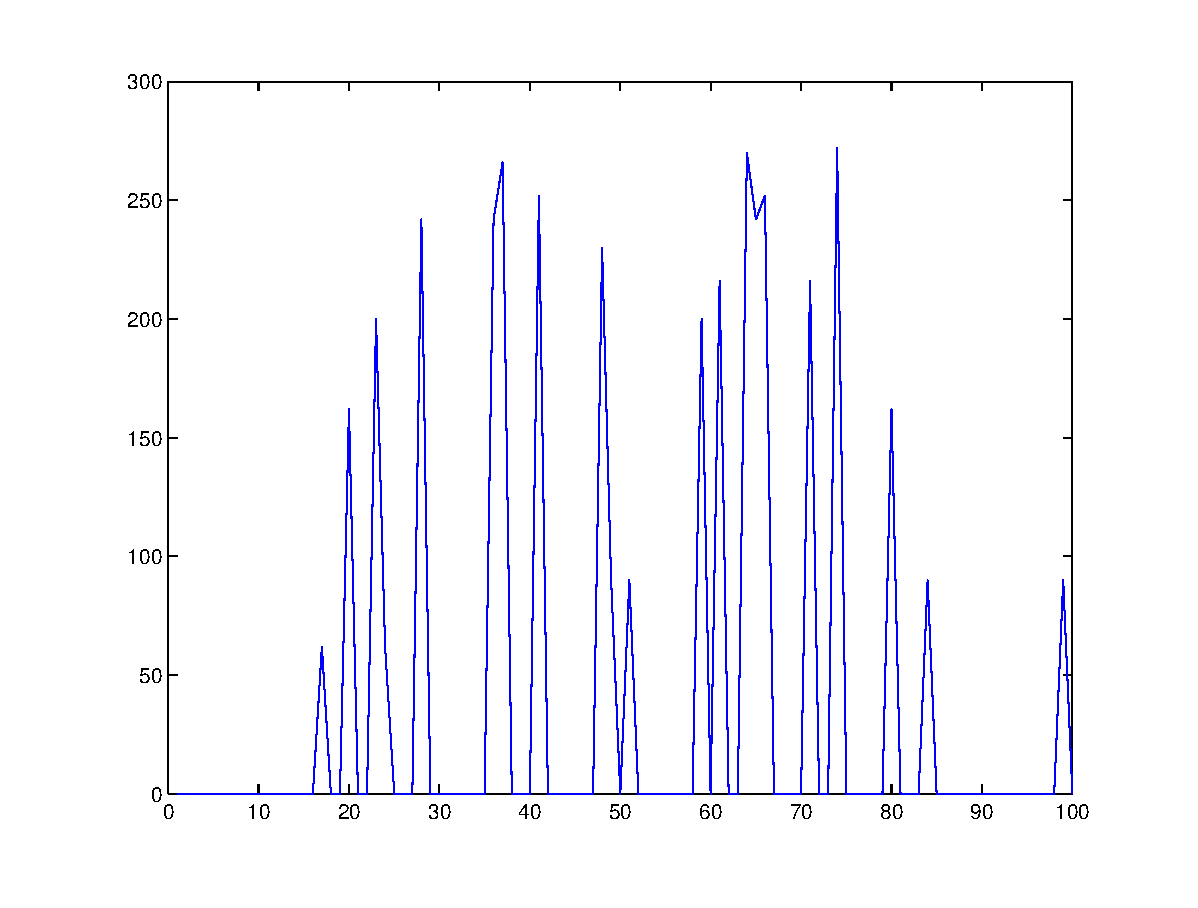
\includegraphics[width=.45\textwidth]{pictures/1_24_16/sine_cpsn_shift18.eps}
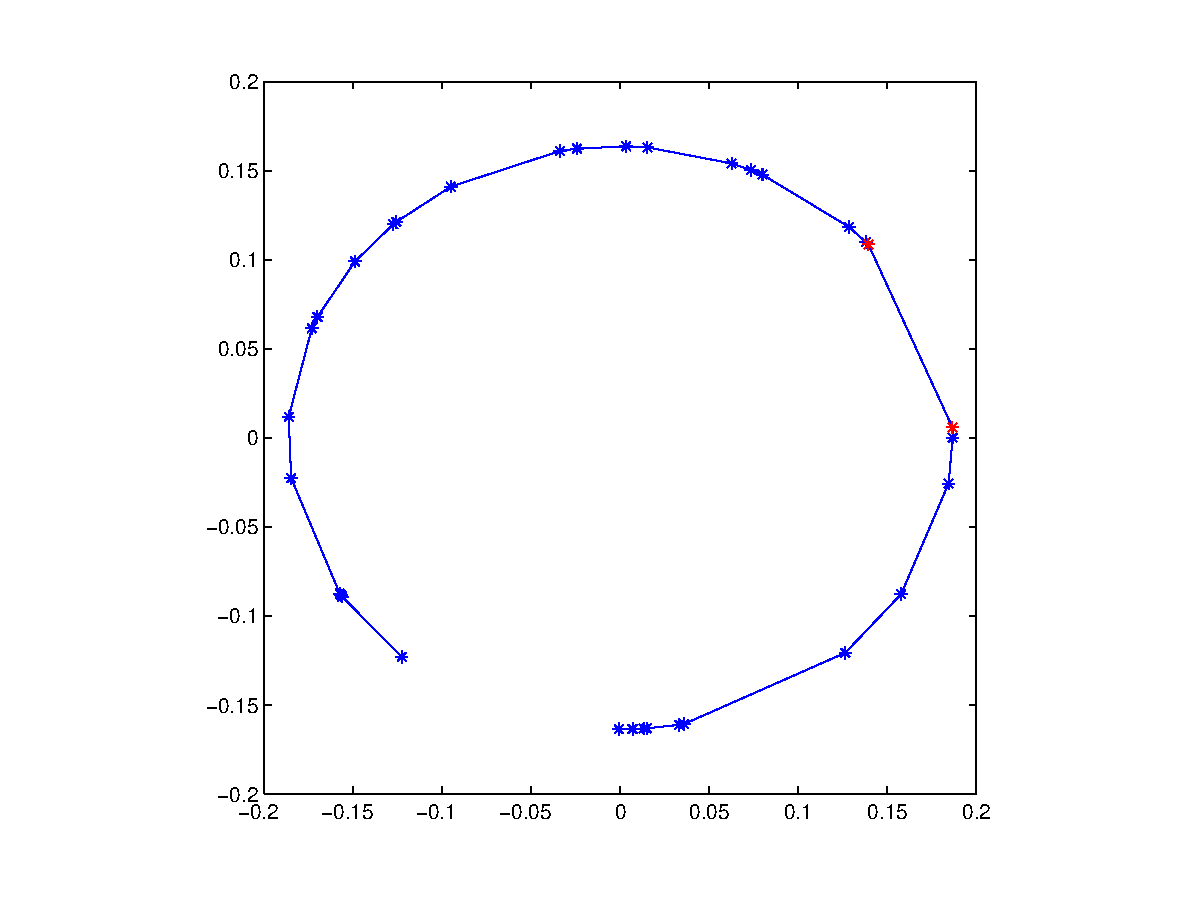
\includegraphics[width=.45\textwidth]{pictures/1_24_16/phases_shift18.eps}
\caption{Left: Algorithm performance when \texttt shift=18. Right: Plot of phases for a permutation which the algorithm had shifted by 11 places (distance = 242). The red asterisks highlight the 11th and 12th points in the cycle.}  
\end{figure}
The algorithm determines the starting point by finding the largest gap between points in the phase plot (greatest difference in angle). Once the phases are too spread out, the largest gap can easily be between a pair of middle points. Note, however, that still the algorithm cycles in the correct direction in each case. 


\section{Listings}
\lstset{language=Matlab, caption=cyclic\_distance}
\begin{lstlisting}[frame=single]
function [dist] = cyclic_distance(V1, V2)
[~, ss] = sort([V1(:), V2(:)]);
dist = sum(abs(diff(ss,1,2)))/2;
\end{lstlisting}

\subsection{Movies}
\subsubsection{Data Treatment}
In the original data set, there are gaps in the data for some genres and not all genres began at the same time so some initial data treatment was required. First, years in which there were gaps in the data were inpainted using linear interpolation. Next, the genre counts were taken on a log scale to account for the fact that movie production has grown exponentially. Finally, only years in which genres had data points were considered (1916-2015). The film-noir genre had to be excluded since the production years were so limited.
The following table shows the results of \verb|analyze_cyclicity| on the movie data (processed as described above). 
\begin{figure}[H]
\begin{minipage}{.3\textwidth}
\csvautotabular{tables/genre_results.txt}
\end{minipage}
\hfill
\begin{minipage}{.65\textwidth}
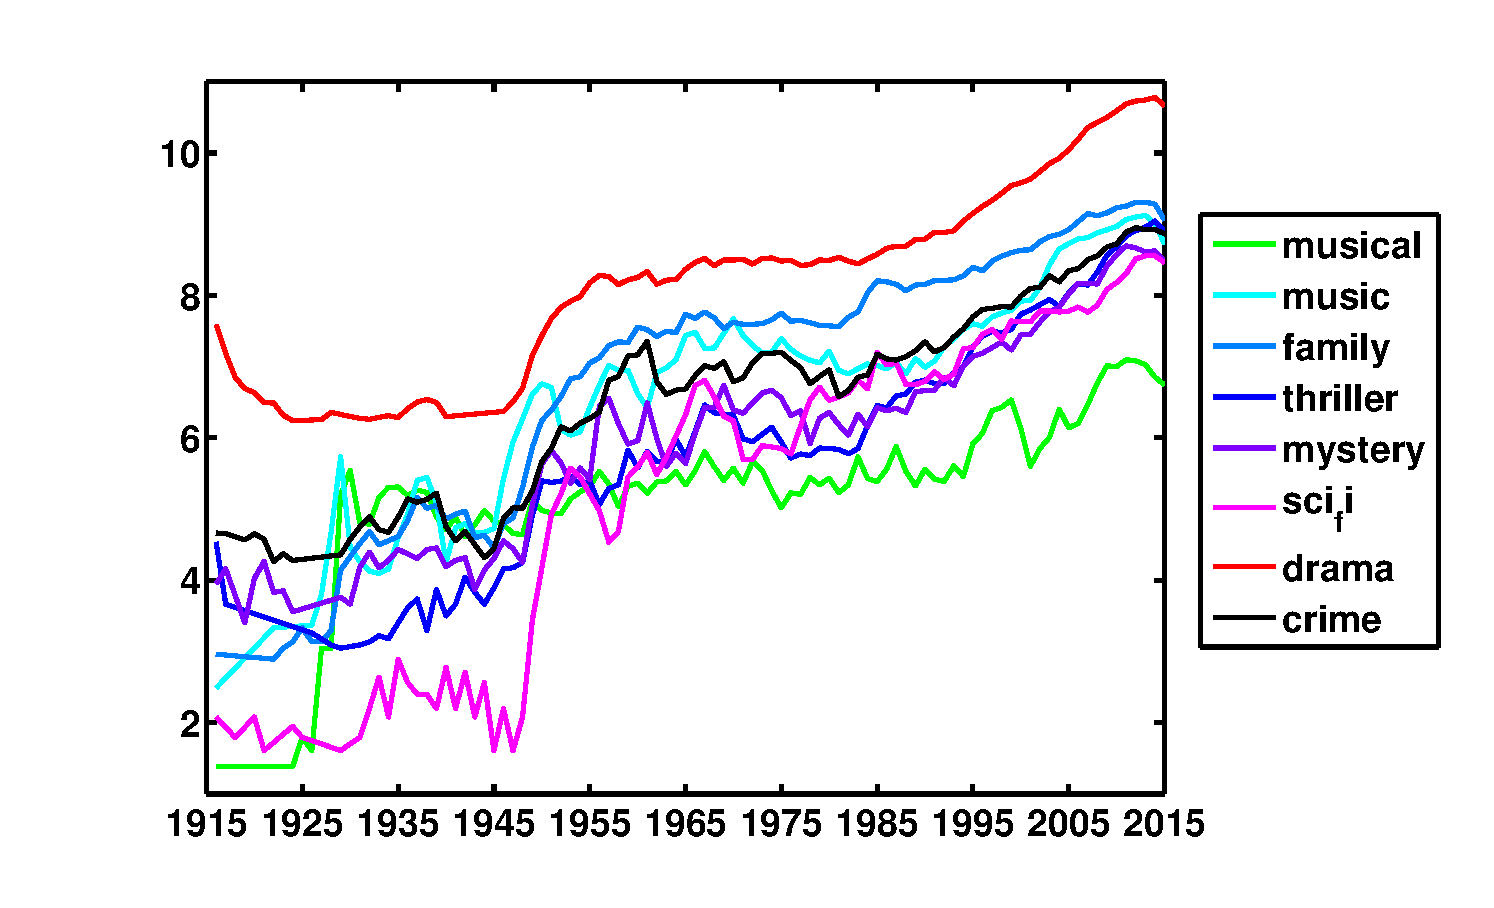
\includegraphics[width=\textwidth]{pictures/movie_data_all_yrs.eps}
\caption{Traces from the first eight genres.}
\end{minipage}
\end{figure}
\begin{figure}[H]
\centering
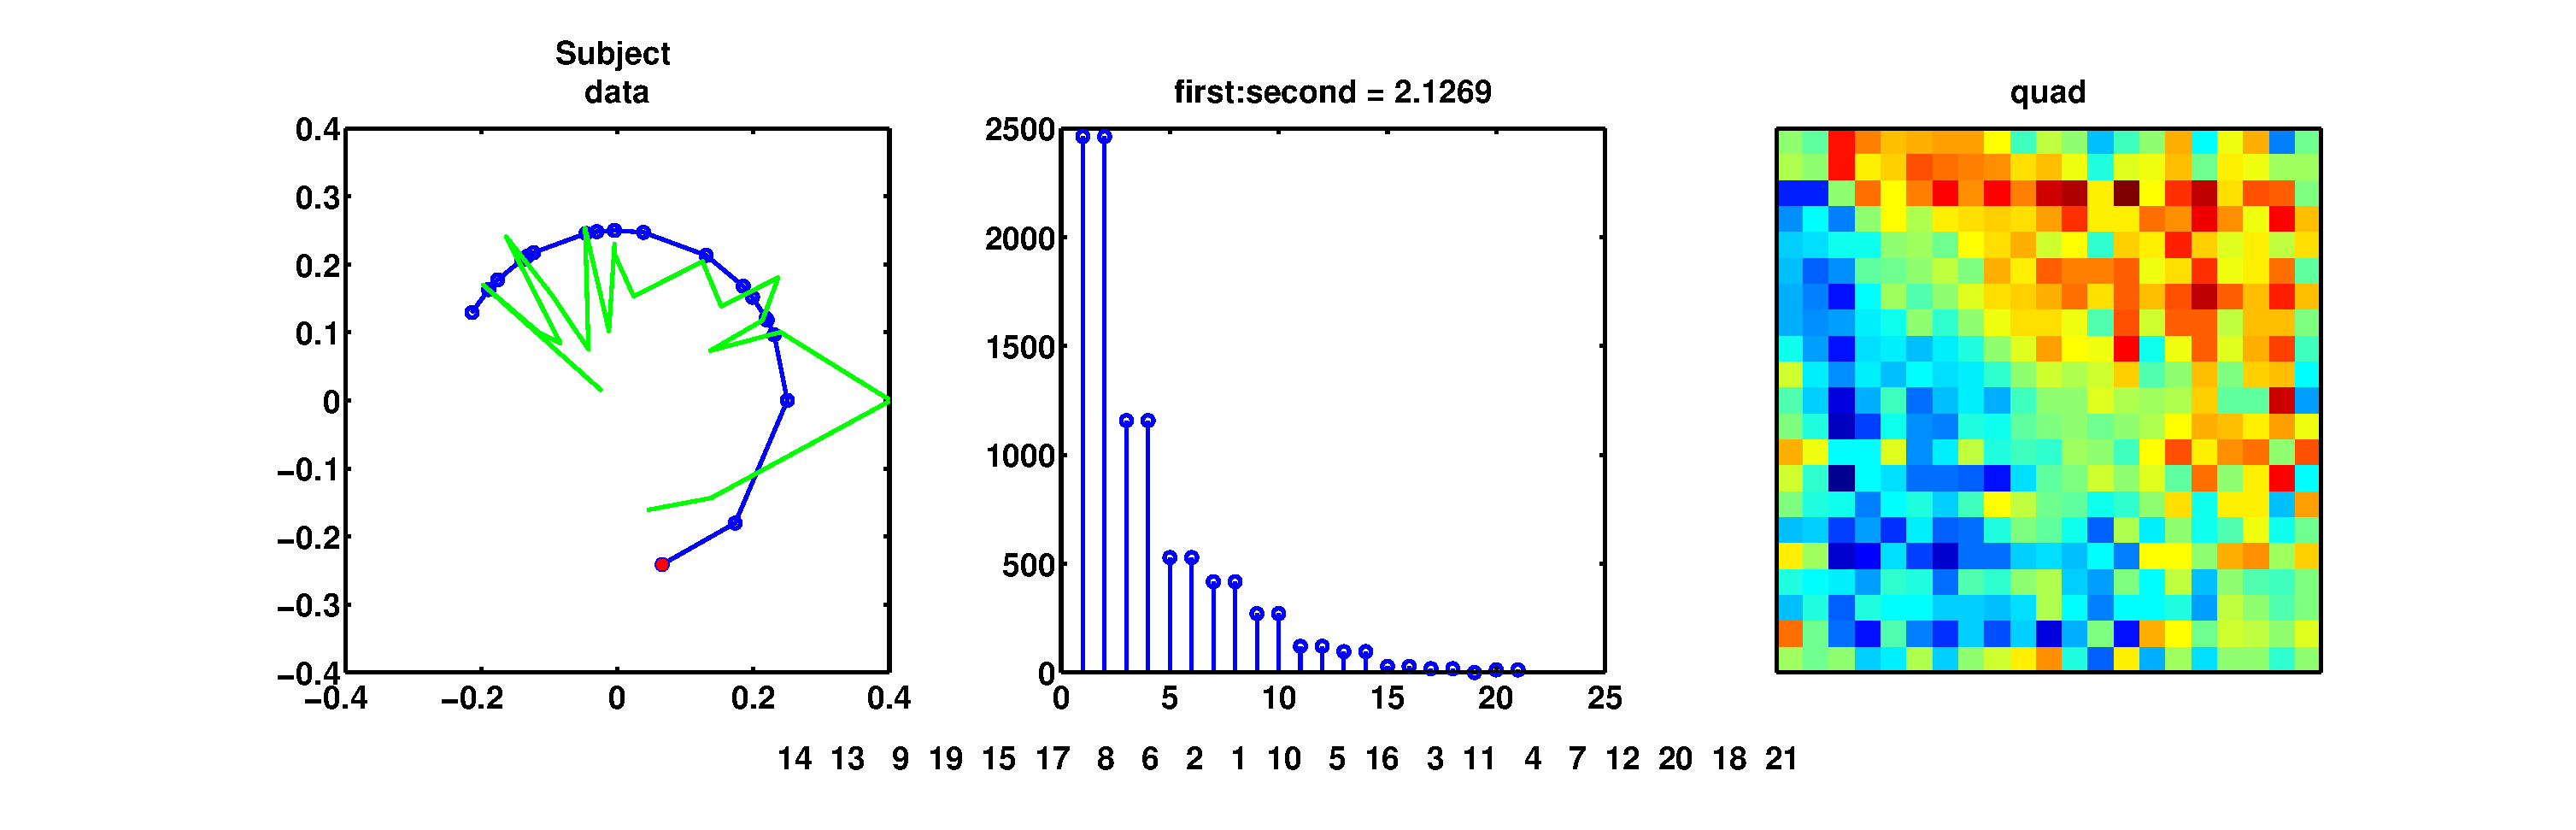
\includegraphics[trim= 130 0 130 0, clip, width=\textwidth]{pictures/movie_data_QC.eps}
\caption{Cyclicity results using quadratic variation normalization}
\end{figure}
Note that the Musicals and Music genres look very similar to each other, but dissimilar to everything else and show a drastic jump around 1925. Since this is such a long time ago, it seemed worth considering more recent trends in the data.
\begin{figure}[H]
\begin{minipage}{.3\textwidth}
\csvautotabular{../Movies/Recent_data/Results/genre_results_table.txt}
\end{minipage}
\hfill
\begin{minipage}{.6\textwidth}
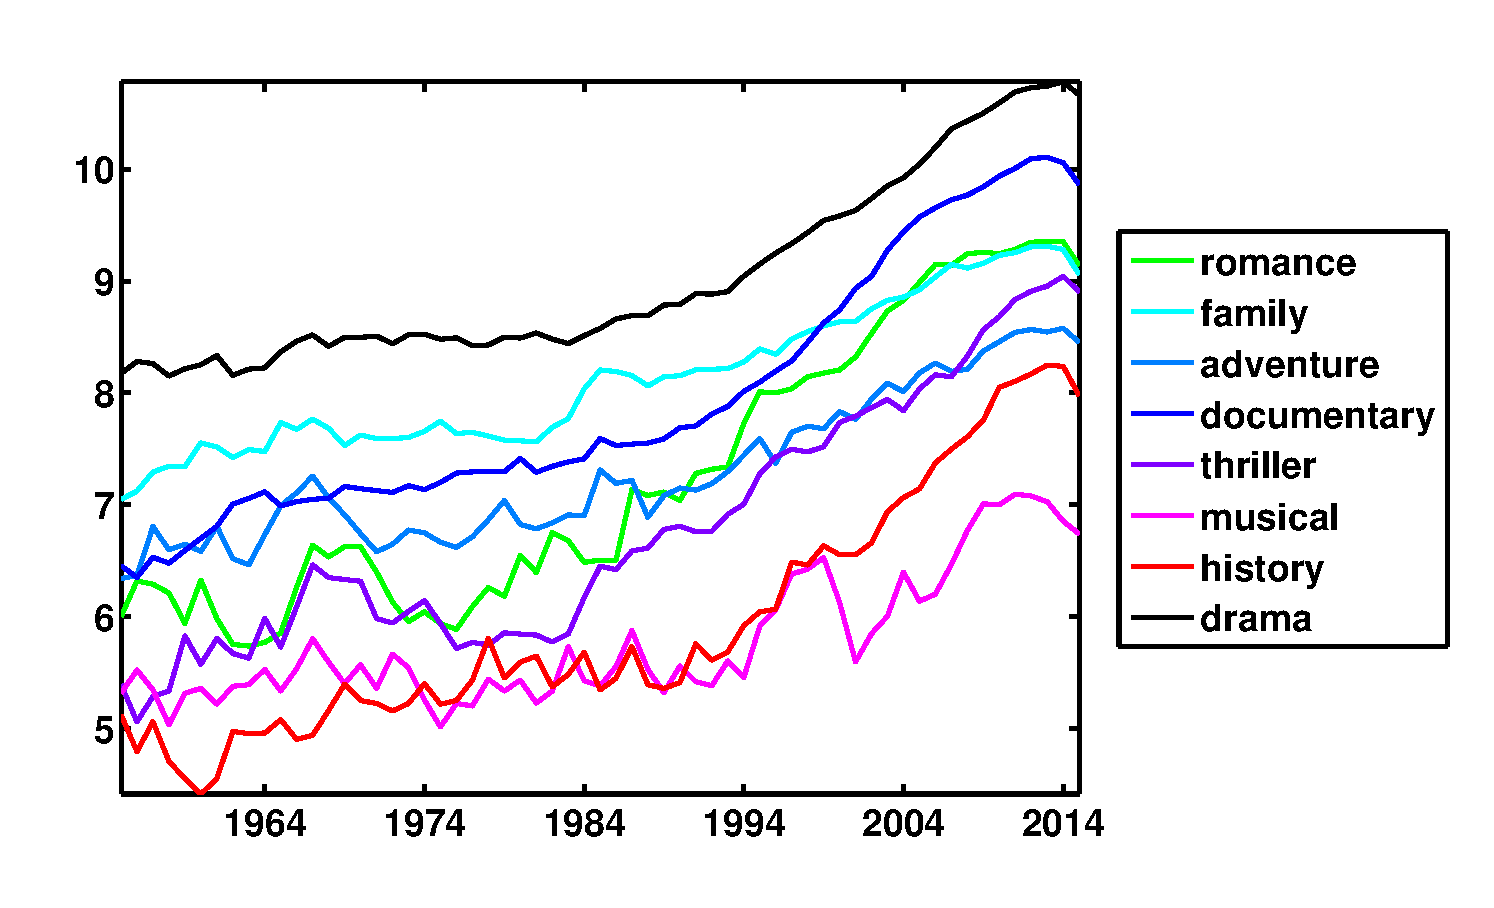
\includegraphics[width=\textwidth]{pictures/movie_data_1955-2015.eps}
\caption{Traces from the first eight genres using only years 1955-2015 in the cyclicity calculation.}
\end{minipage}
\end{figure}
\begin{figure}[H]
\centering
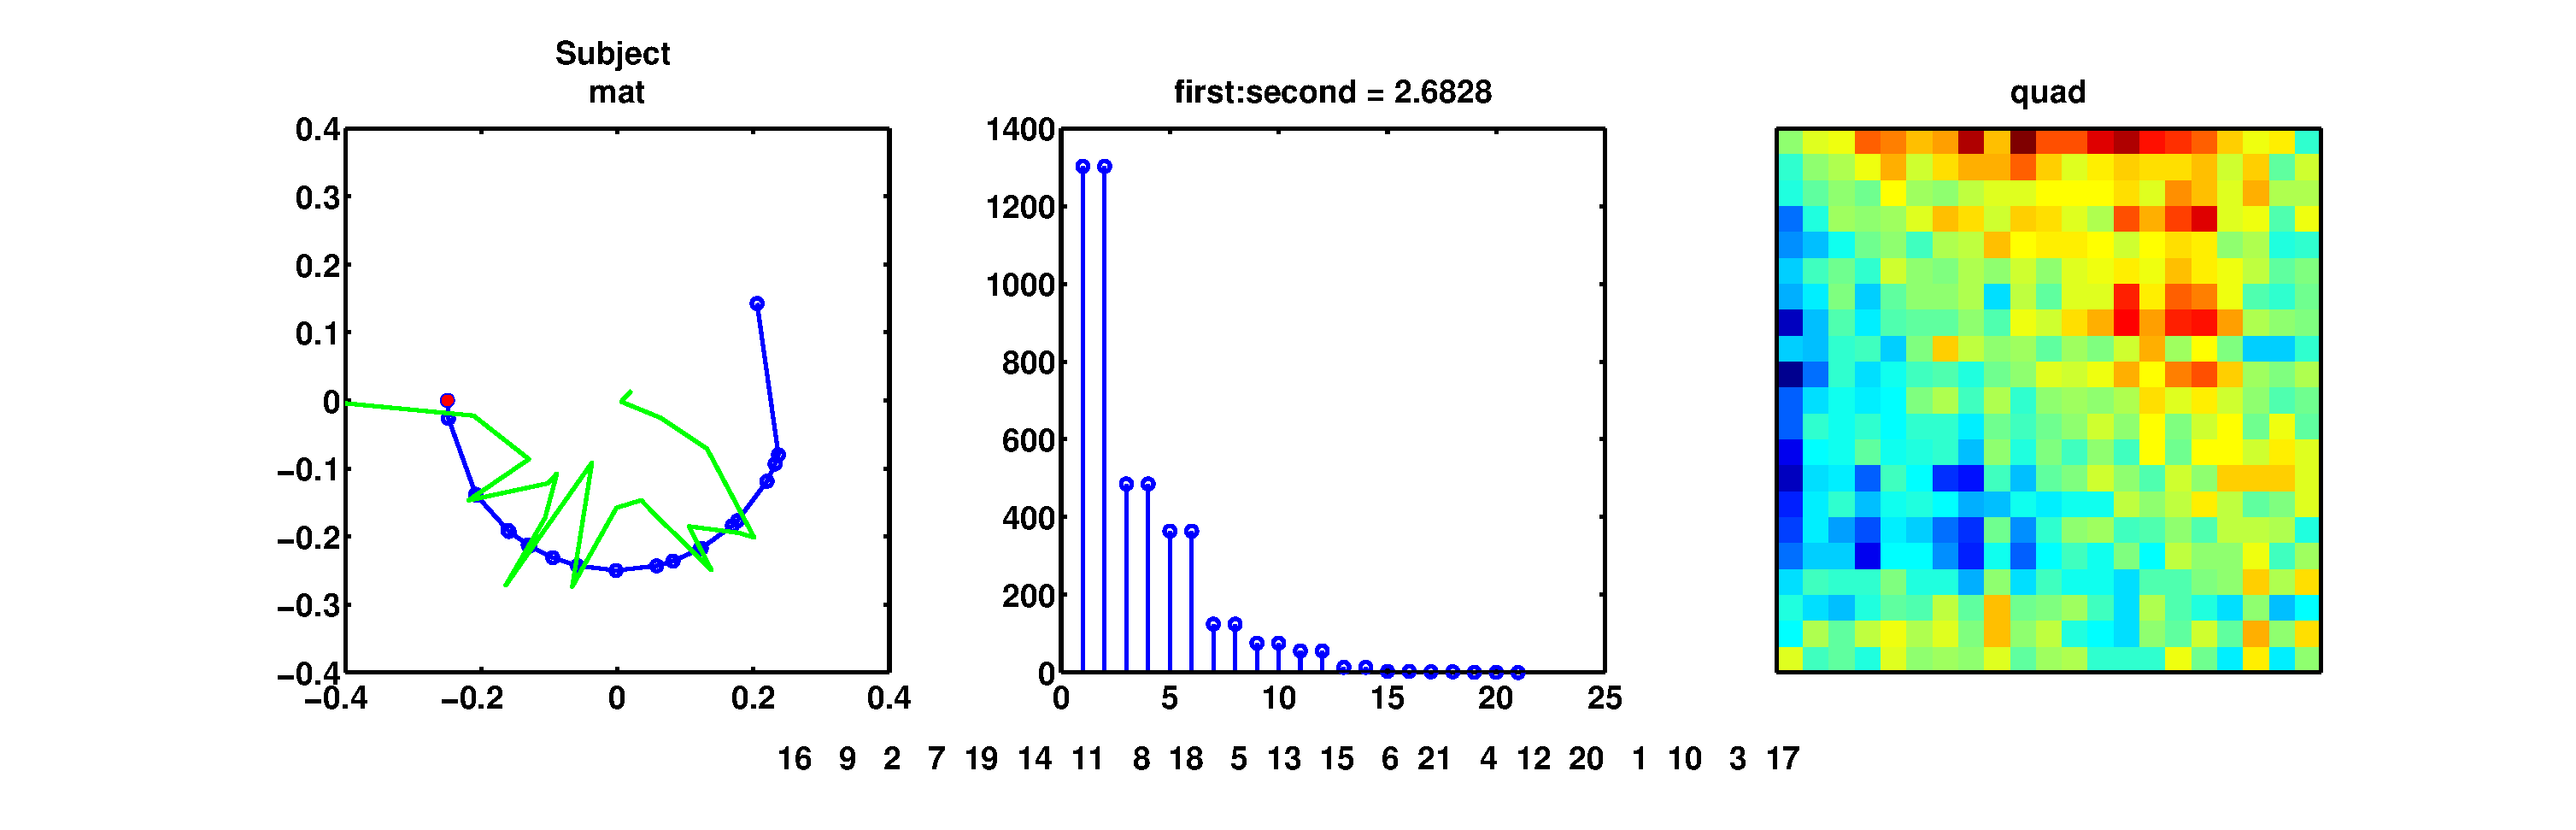
\includegraphics[trim= 130 0 130 0, clip, width=\textwidth]{pictures/movie_data_1955-2015_QC.eps}
\caption{Cyclicity results from 1955-2015 movie data using quadratic variation normalization}
\end{figure}

\section{2/2/16}
\subsection{Movie trends with words counts from New York Times}

We added some word trends to the movie data, taking search counts for selected words on the New York Times website. The search was filtered by year so that we could get word counts for each year that we have movie data for (1916-2015). Word counts were pulled using \verb|times_scrape.py| and looping through the years in a bash script (see scraping folder in Movies). The words searched were searched

\begin{center}
\begin{tabular}{lllll}
crisis&
terror&
war&
attack&
expansion\\
growth&
invasion&
prosperity&
shooting&
\end{tabular}
\end{center}

and the following results obtained:

\begin{figure}[H]
\centering
\begin{minipage}{.25\textwidth}
\csvautolongtable{tables/movie_word_perm_results_p1.txt}
\end{minipage}
\begin{minipage}{.25\textwidth}
\csvautolongtable{tables/movie_word_perm_results_p2.txt}
\end{minipage}
\begin{minipage}{.25\textwidth}
\csvautolongtable{tables/movie_word_perm_results_p3.txt}
\end{minipage}
\caption{Resulting permutation from full movie and word analysis}
\end{figure}

\begin{figure}[H]
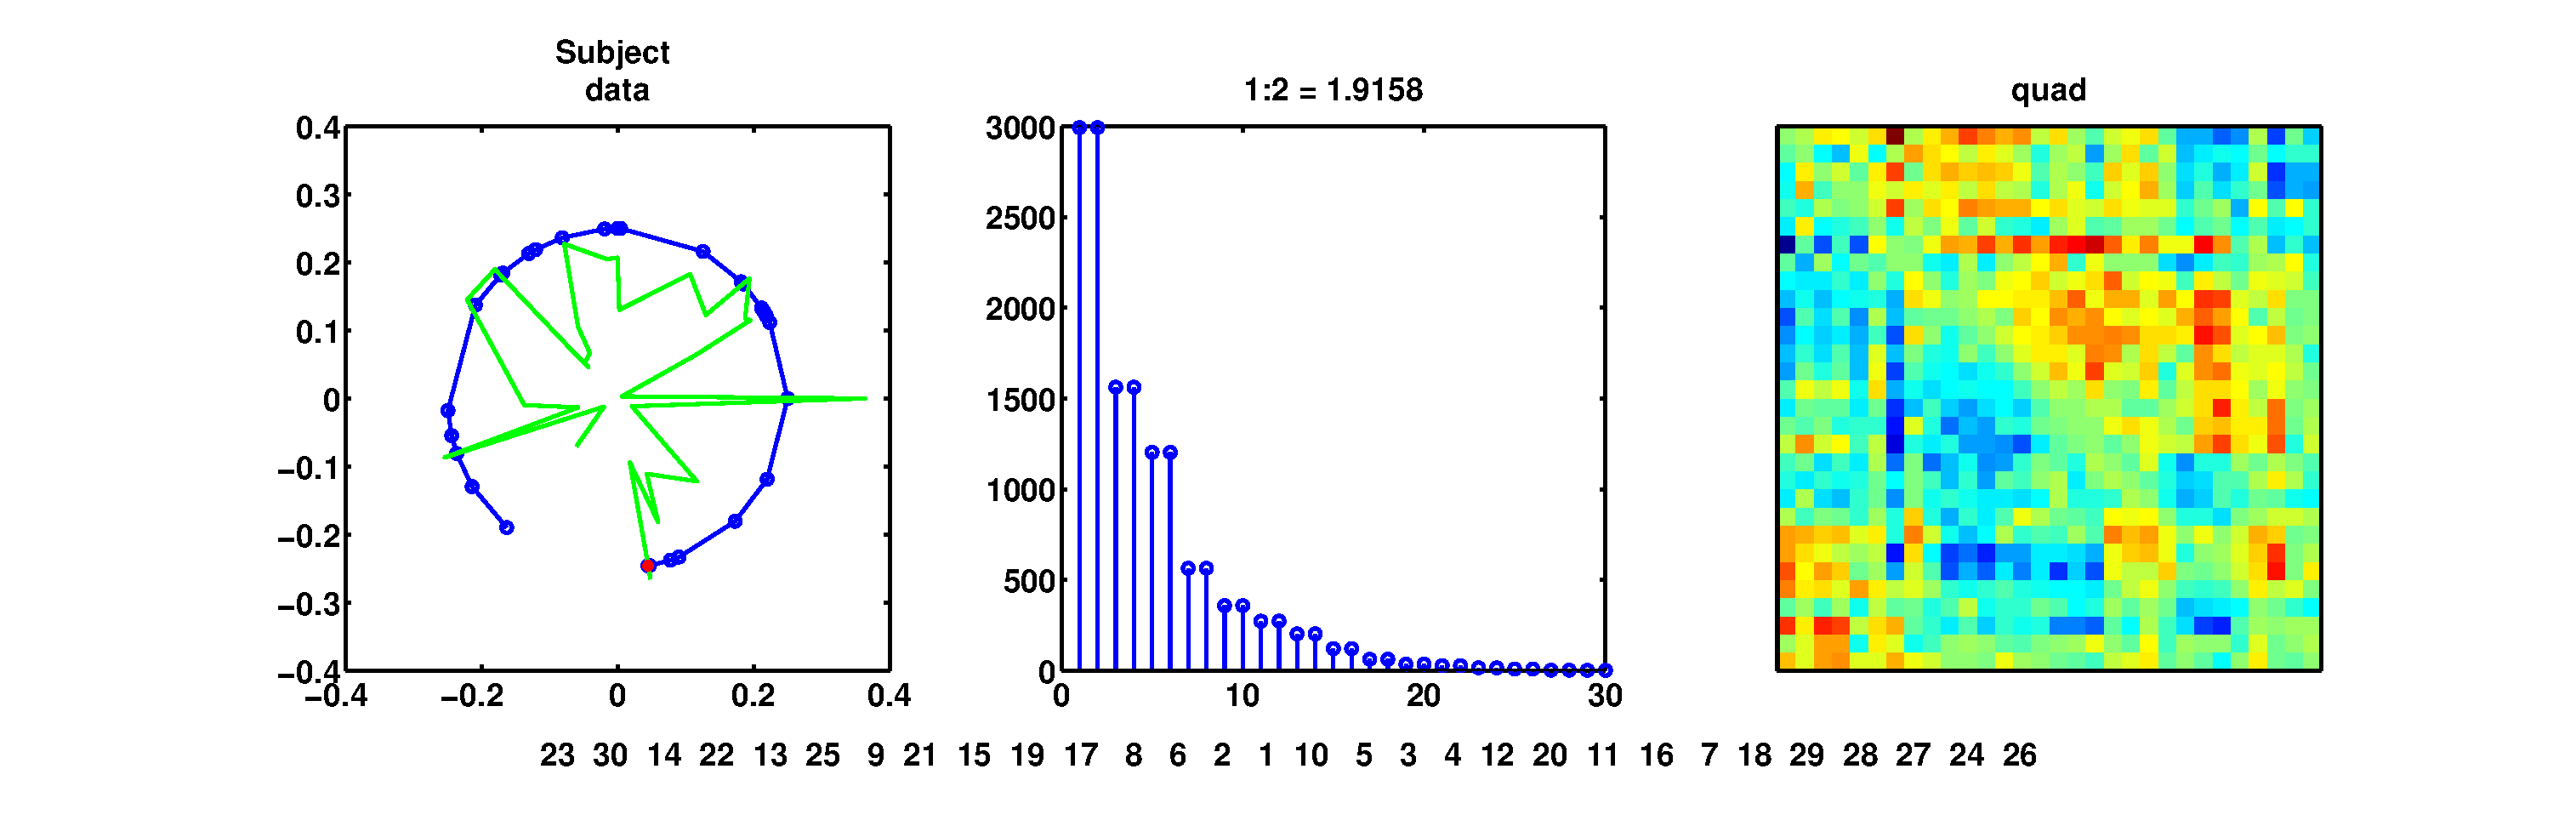
\includegraphics[trim = 150 0 130 0, clip, width=\textwidth]{pictures/movie_word_all.eps}
\caption{Results of full movie and word analysis}
\end{figure}

\subsection{Refining Movie-word results}
Next, we wish to consider smaller subsets of traces using the magnitude of the phase associated with a trace as an indicator of agreement with a particular ordering. For each set of figures, \verb|p| indicates which eigenvector was used to generate the ordering , \verb|n| indicates how many categories were used in the smaller group analysis and \verb|group| is which subset of the full set. So, for example, if \verb|p=1|, \verb|n=8|, \verb|group=1| then the first eigenvector was used to generate an ordering of full set of categories and then the eight categories with the highest magnitude of associated phase vector were pulled out and reanalyzed using the cyclicity algorithm to yield the ordering shown in the legend. If \verb|group=2| the group 1 categories were pulled out of the original data set and then the same procedure was followed, ordering the categories associated with the top eight phases of this smaller subset. When \verb|p=2|, the second eigenvector is used in the cyclicity algorithm to generate the ordering.

\begin{figure}[H]
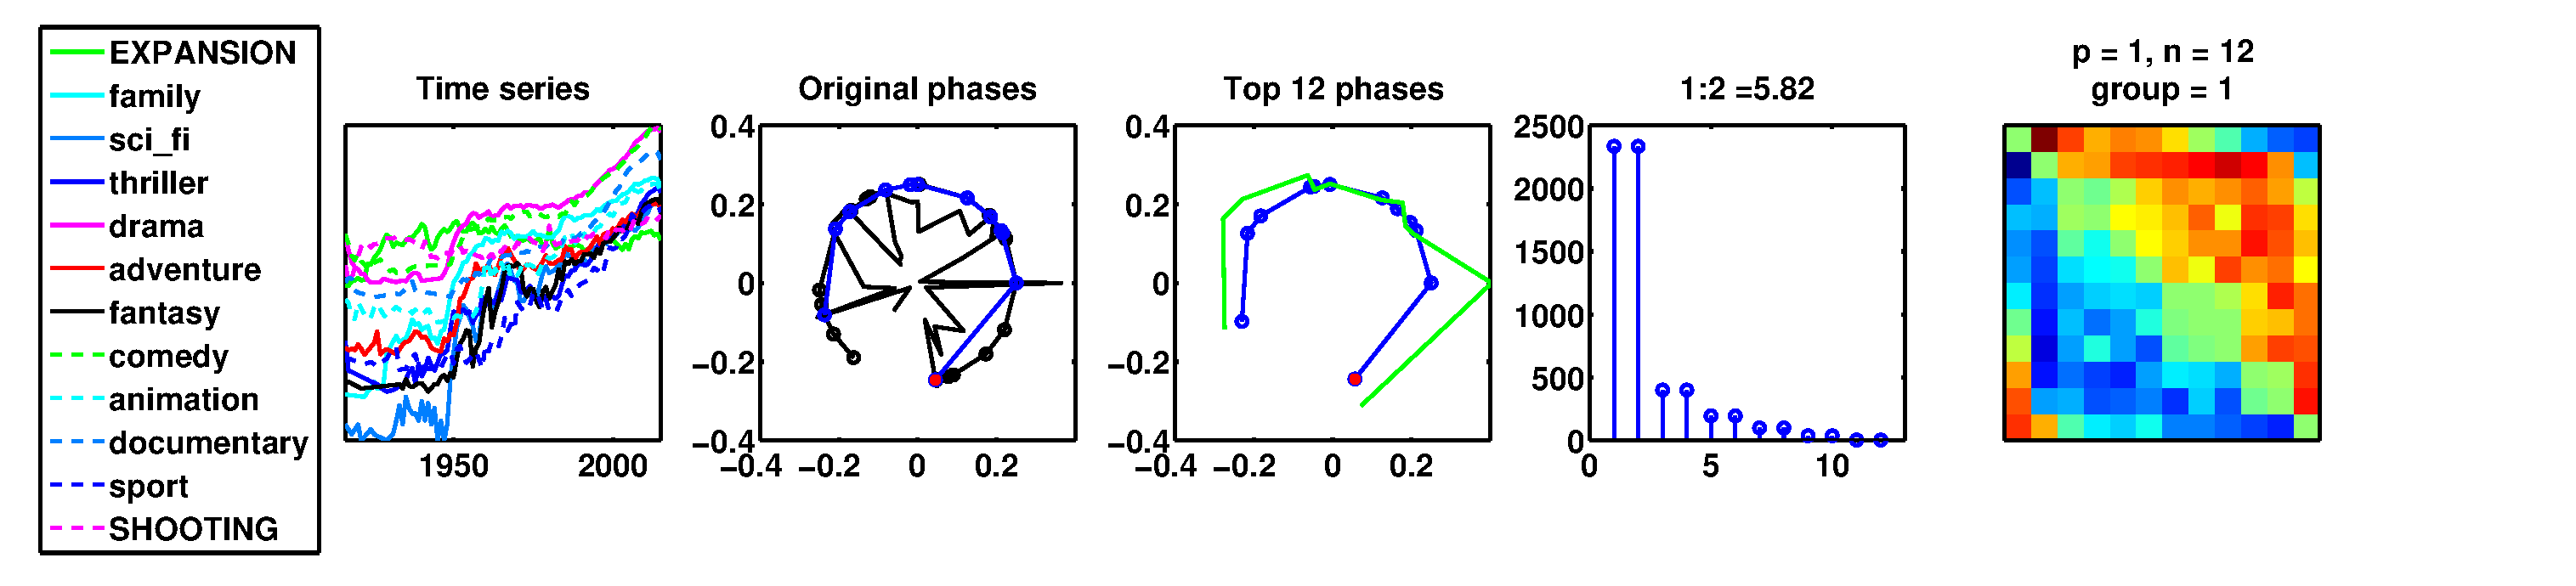
\includegraphics[trim = 0 0 130 0, clip, width=\textwidth]{pictures/_p1_n12_gp1.eps}
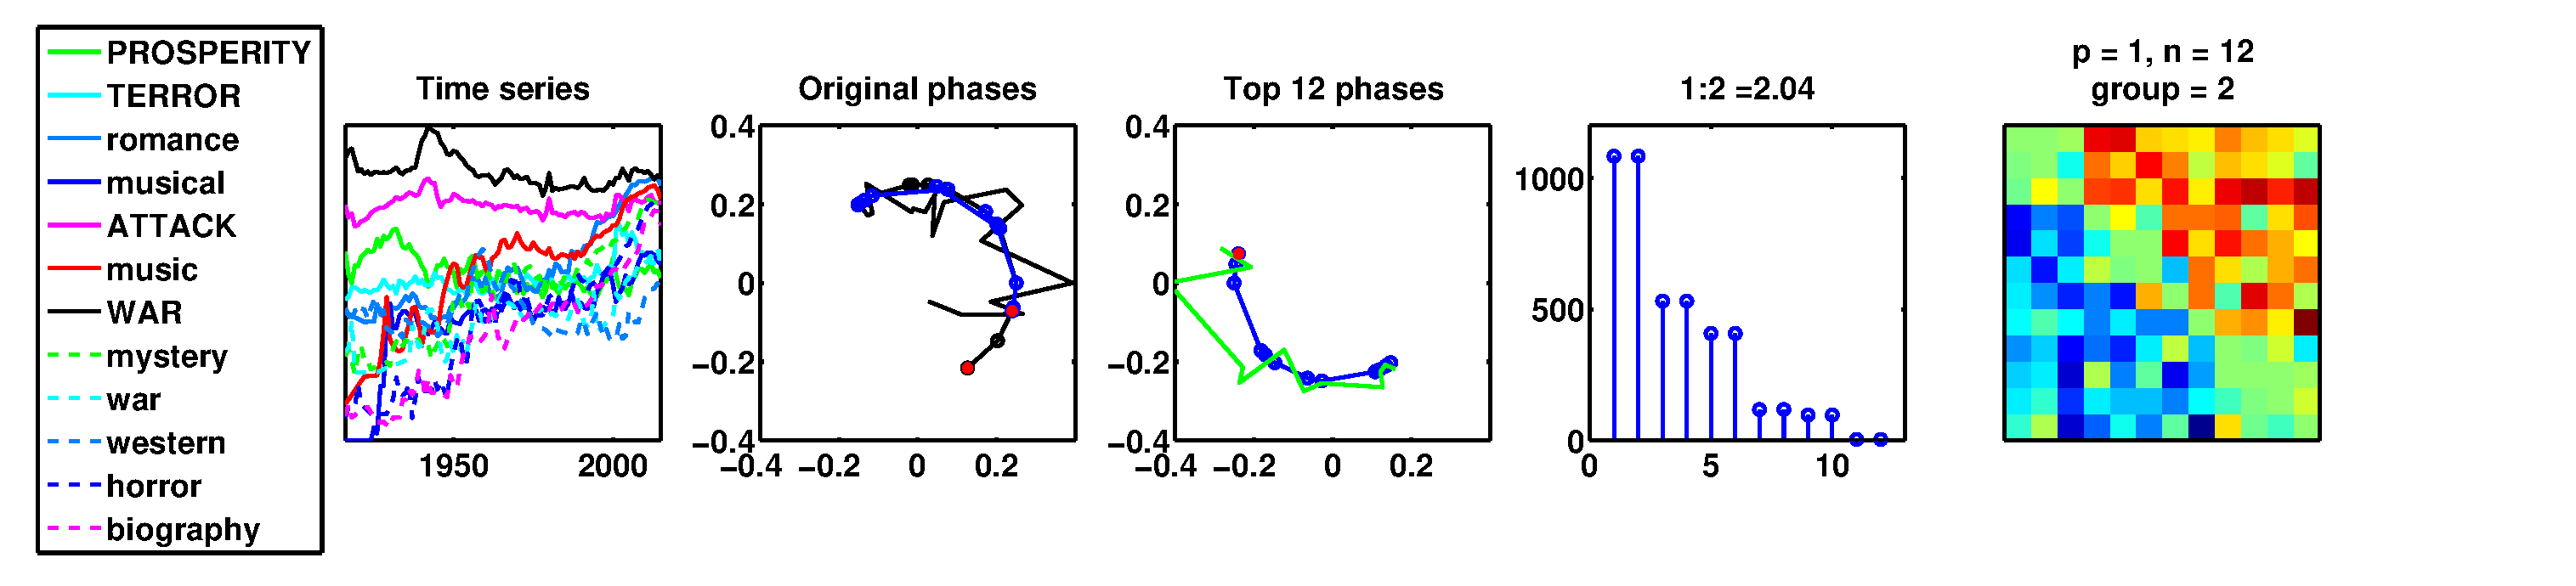
\includegraphics[trim = 0 0 130 0, clip, width=\textwidth]{pictures/_p1_n12_gp2.eps}
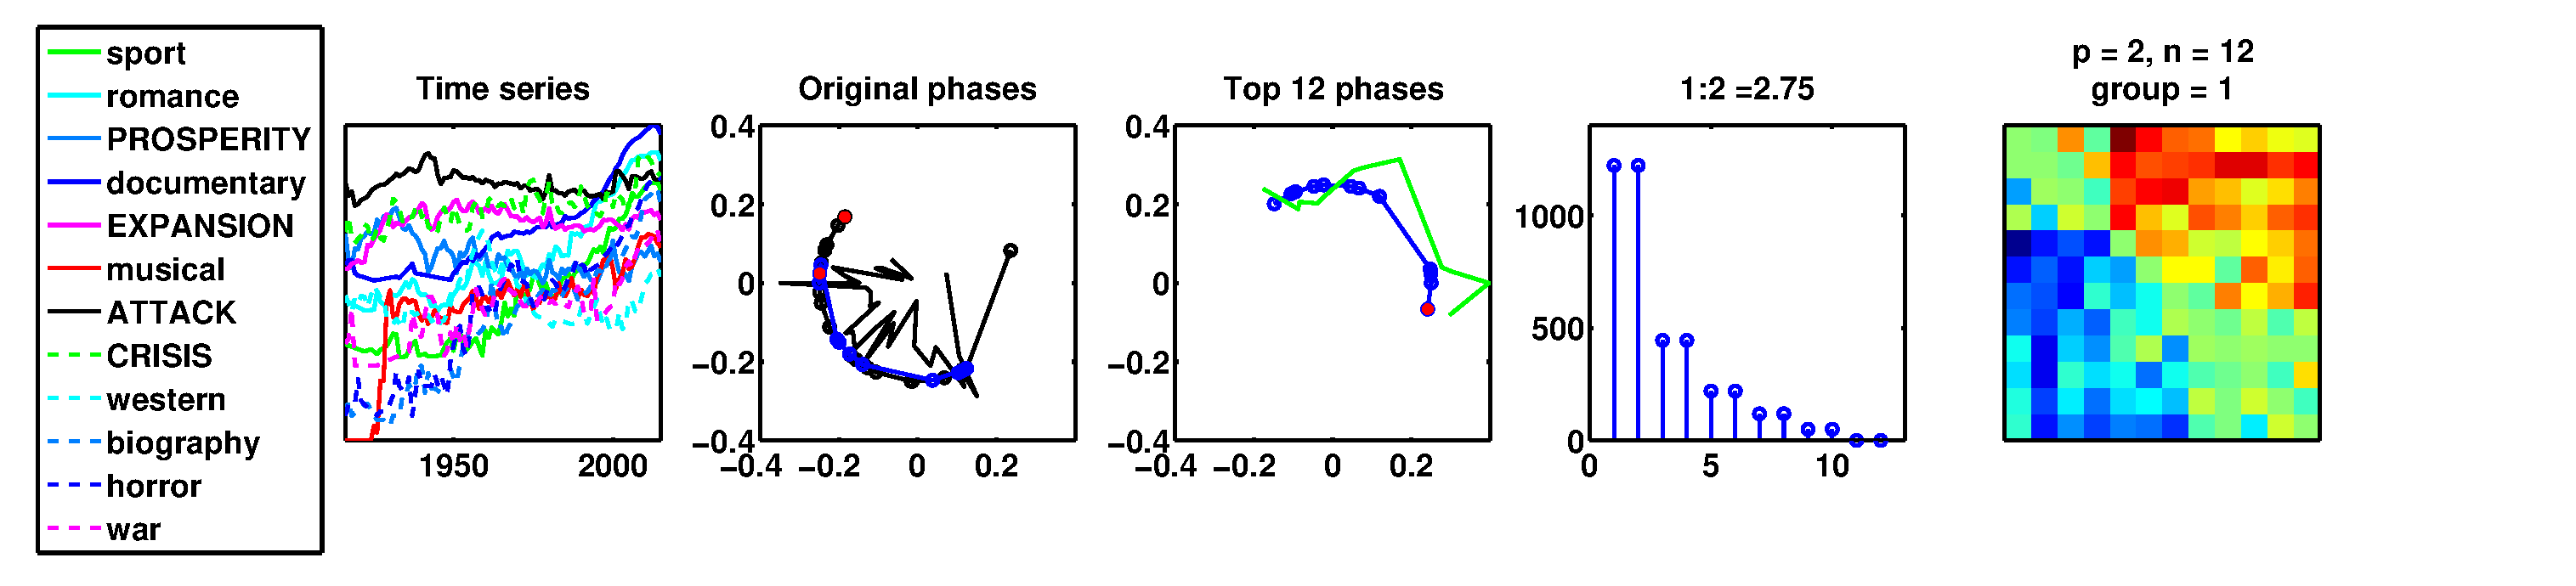
\includegraphics[trim = 0 0 130 0, clip, width=\textwidth]{pictures/_p2_n12_gp1.eps}
\caption{Results with n=12.}
\end{figure}

\begin{figure}[H]
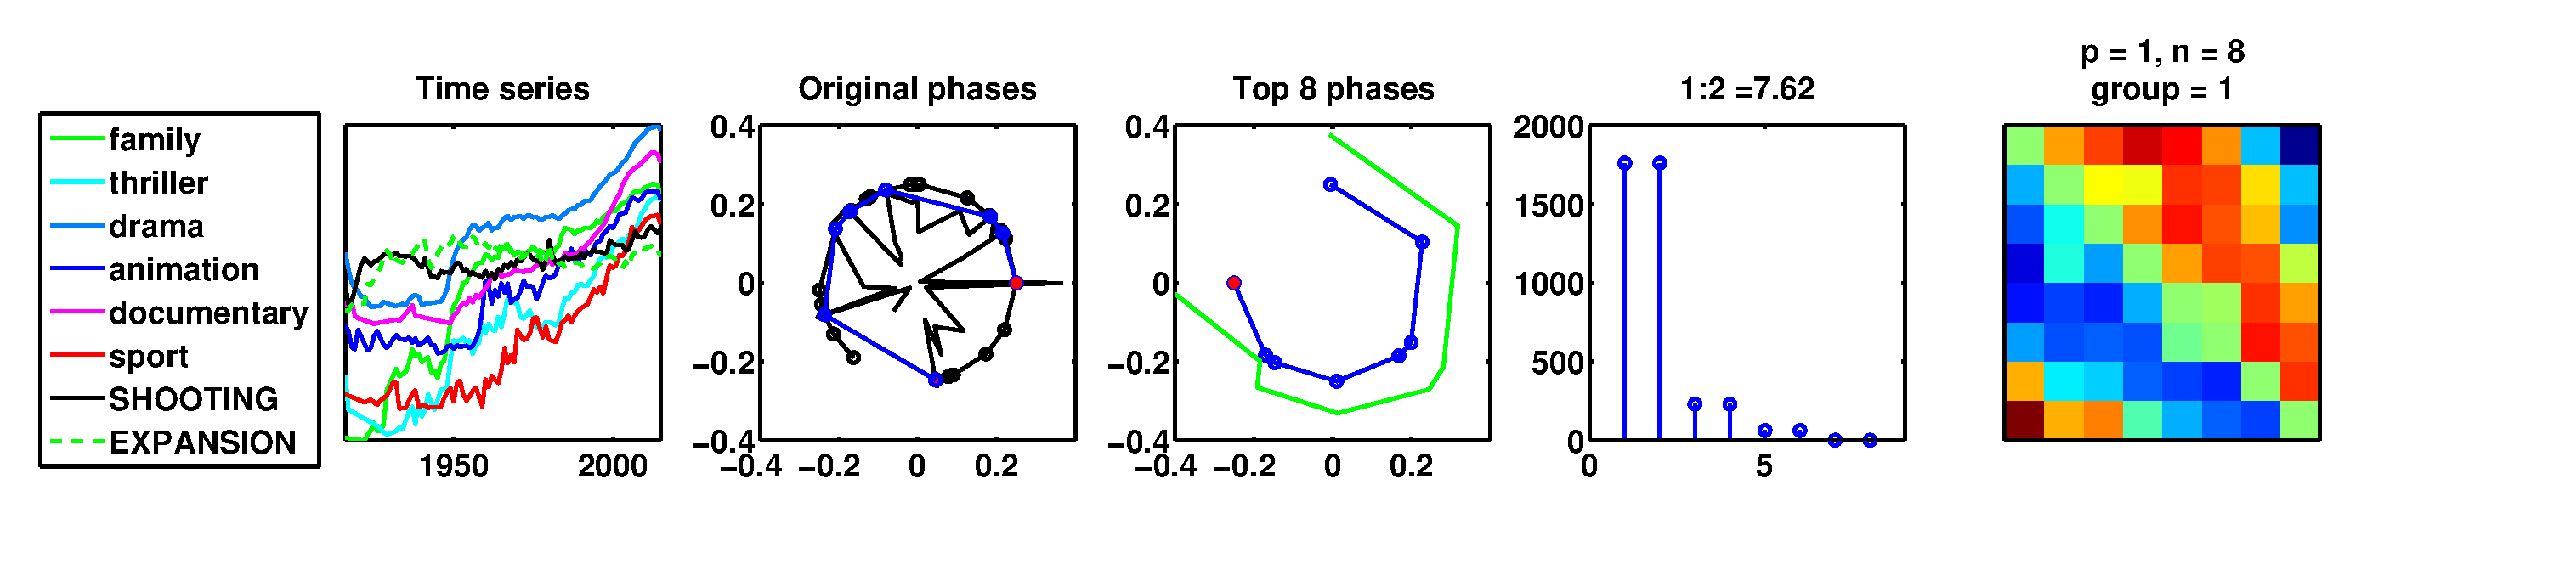
\includegraphics[trim = 0 0 130 0, clip, width=\textwidth]{pictures/_p1_n8_gp1.eps}
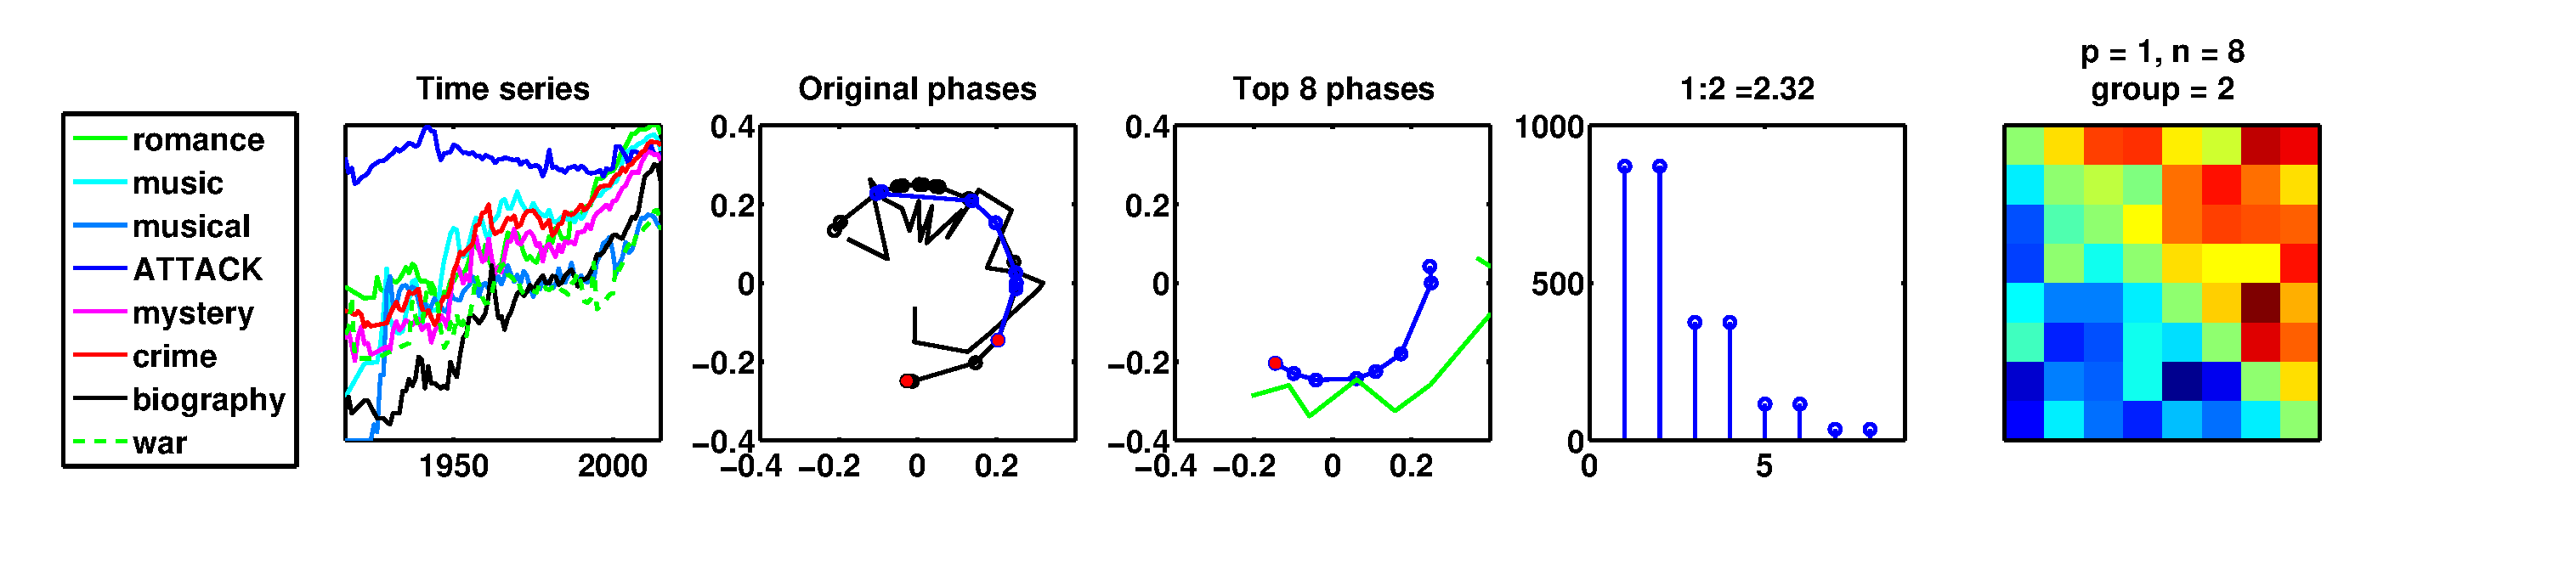
\includegraphics[trim = 0 0 130 0, clip, width=\textwidth]{pictures/_p1_n8_gp2.eps}
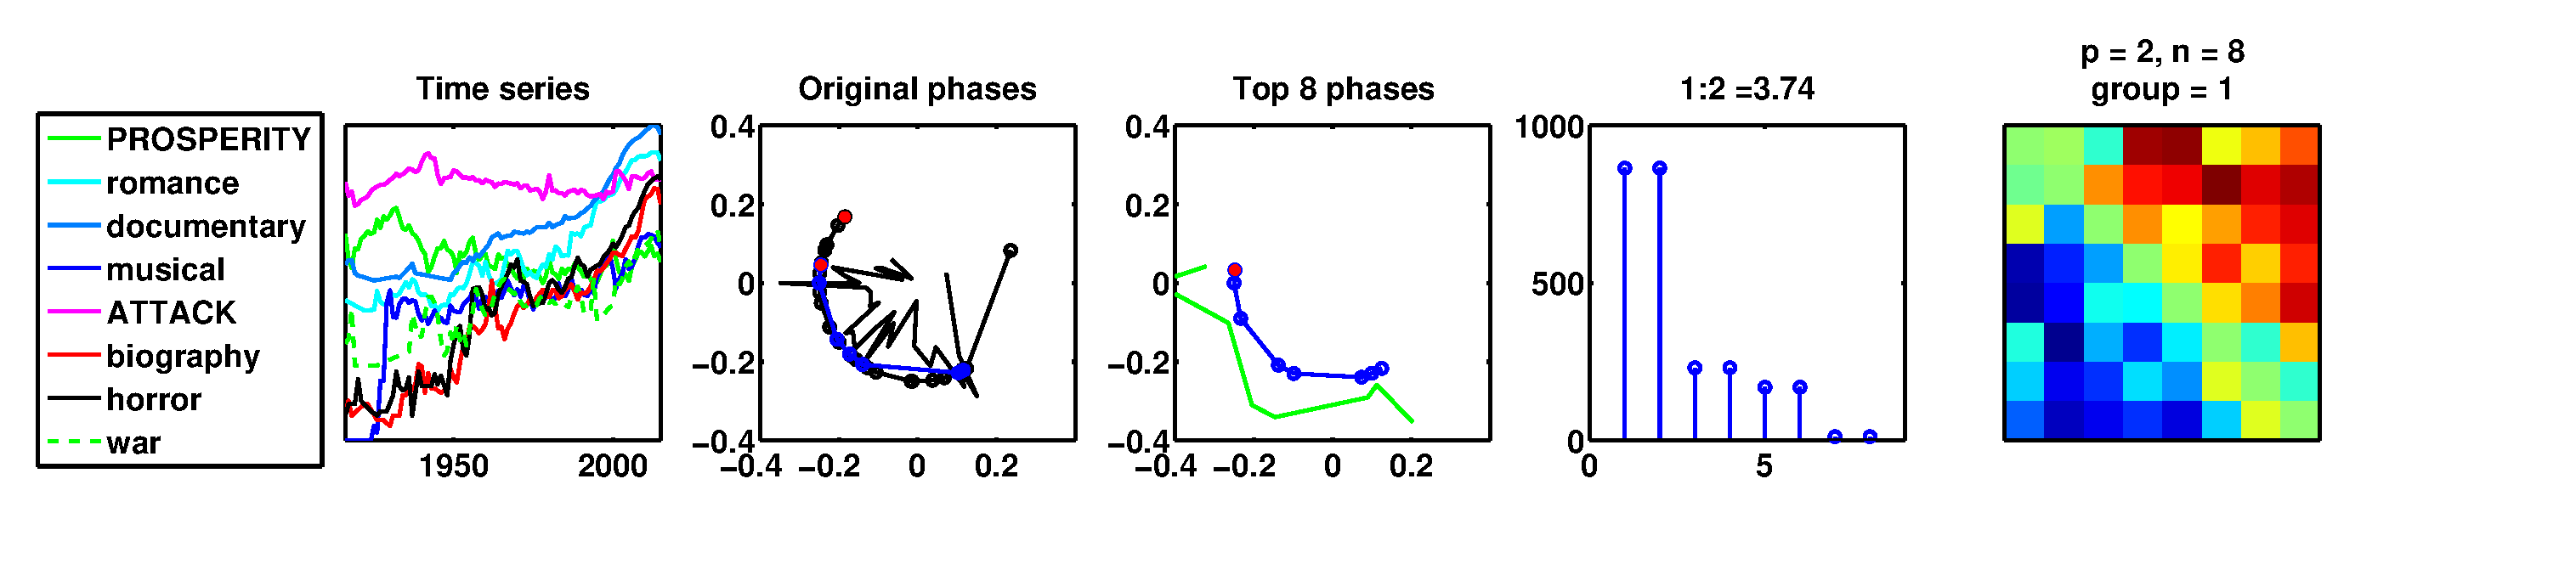
\includegraphics[trim = 0 0 130 0, clip, width=\textwidth]{pictures/_p2_n8_gp1.eps}
\caption{Results with n=8.}
\end{figure}

\begin{figure}[H]
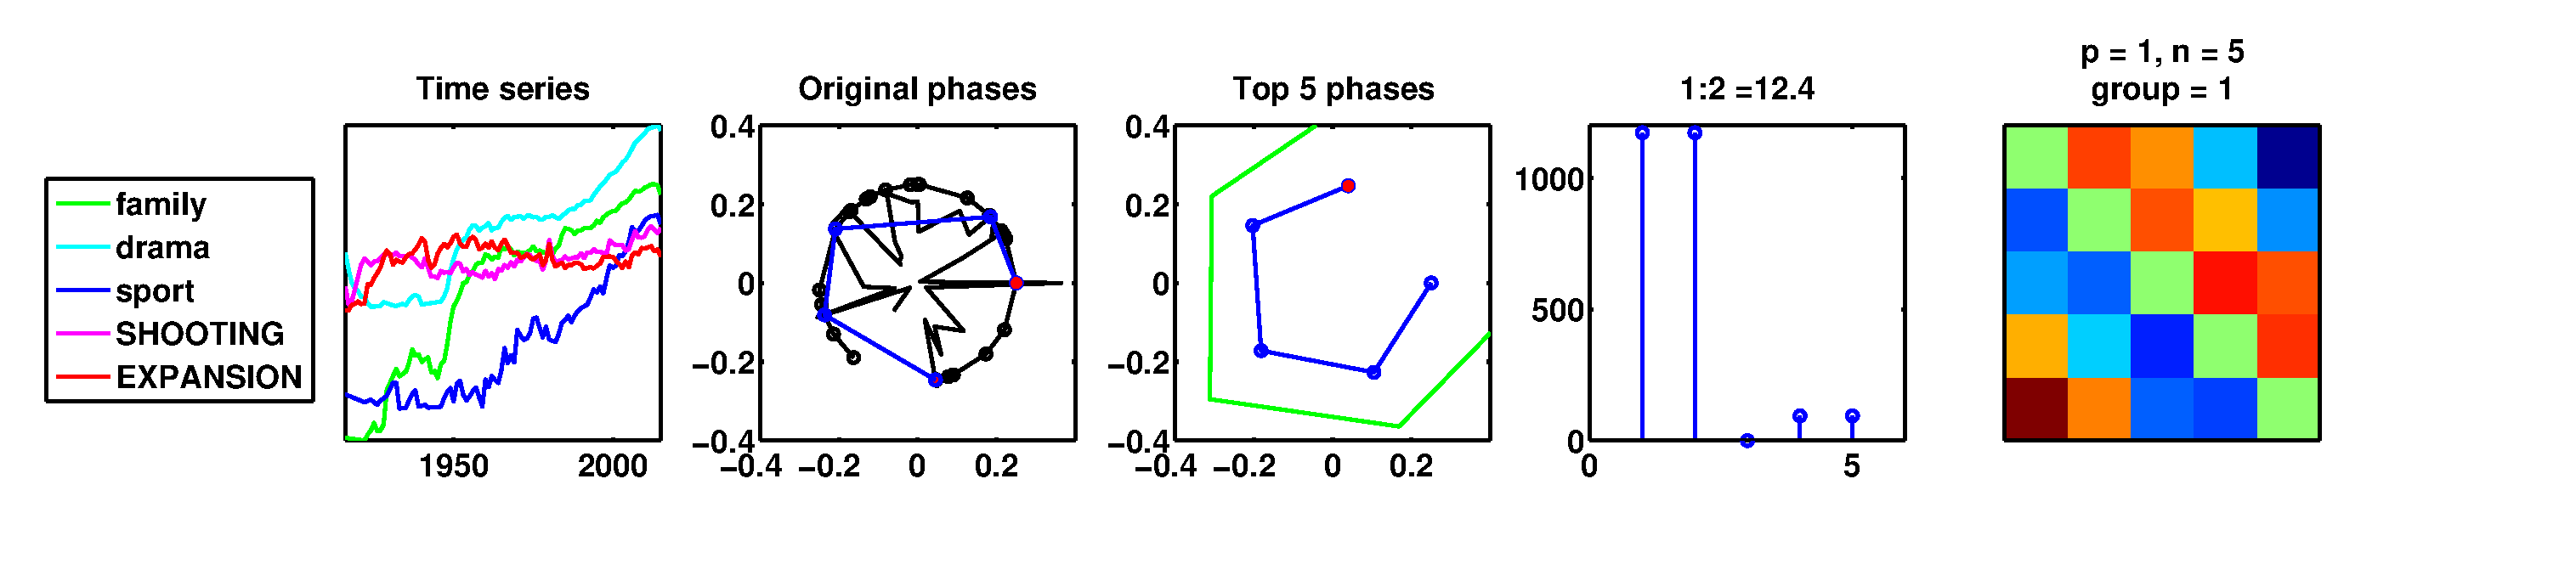
\includegraphics[trim = 0 0 130 0, clip, width=\textwidth]{pictures/_p1_n5_gp1.eps}
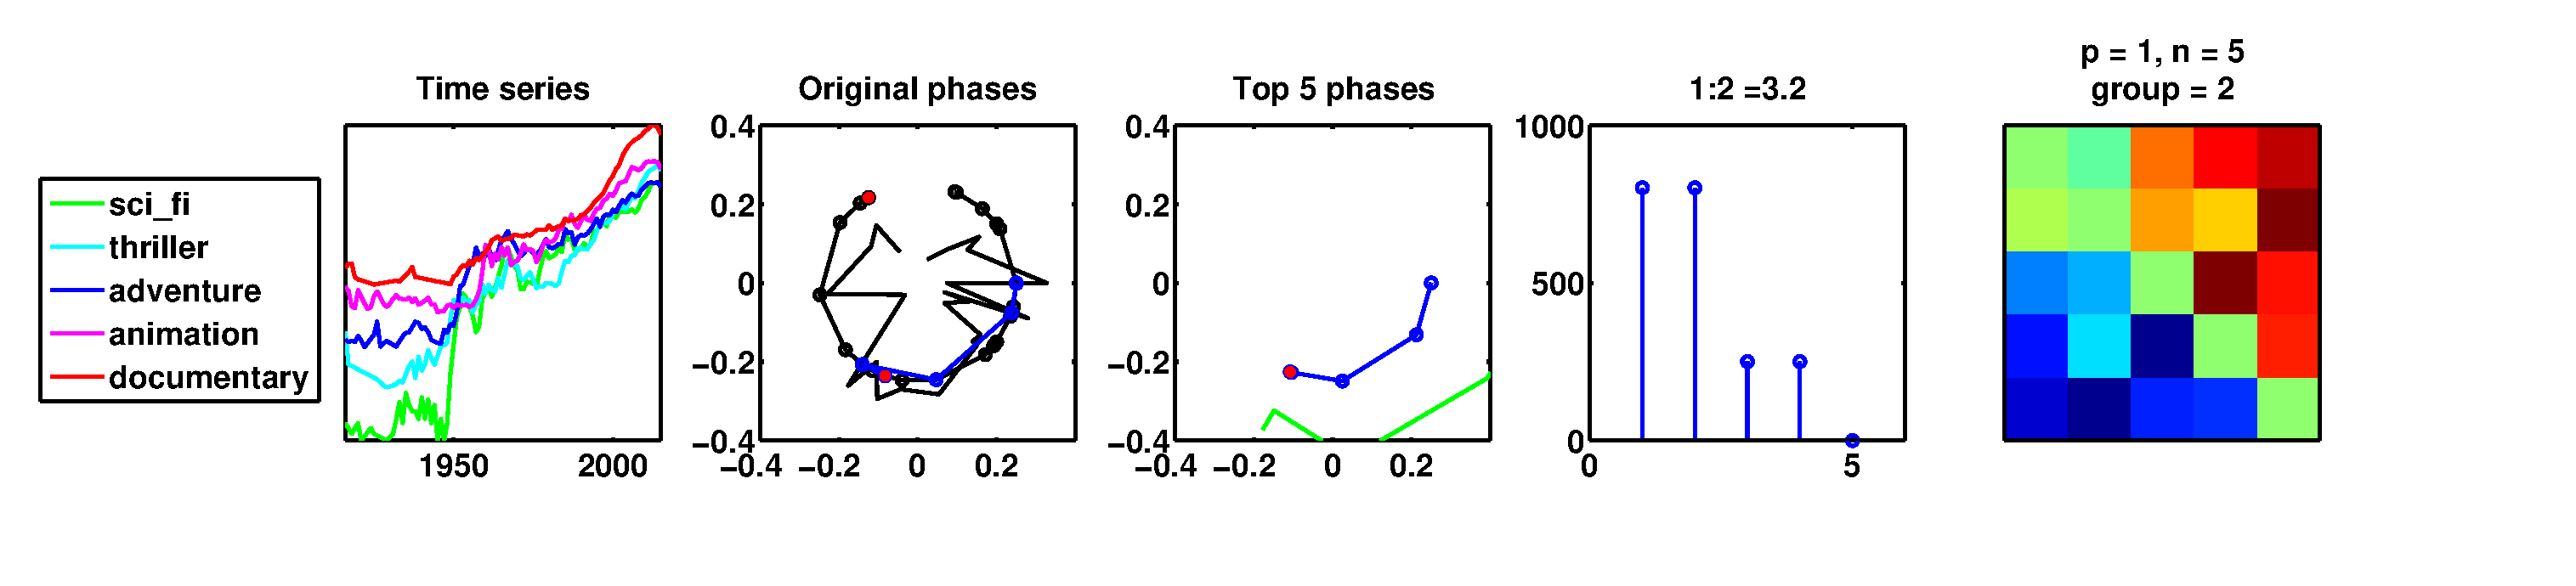
\includegraphics[trim = 0 0 130 0, clip, width=\textwidth]{pictures/_p1_n5_gp2.eps}
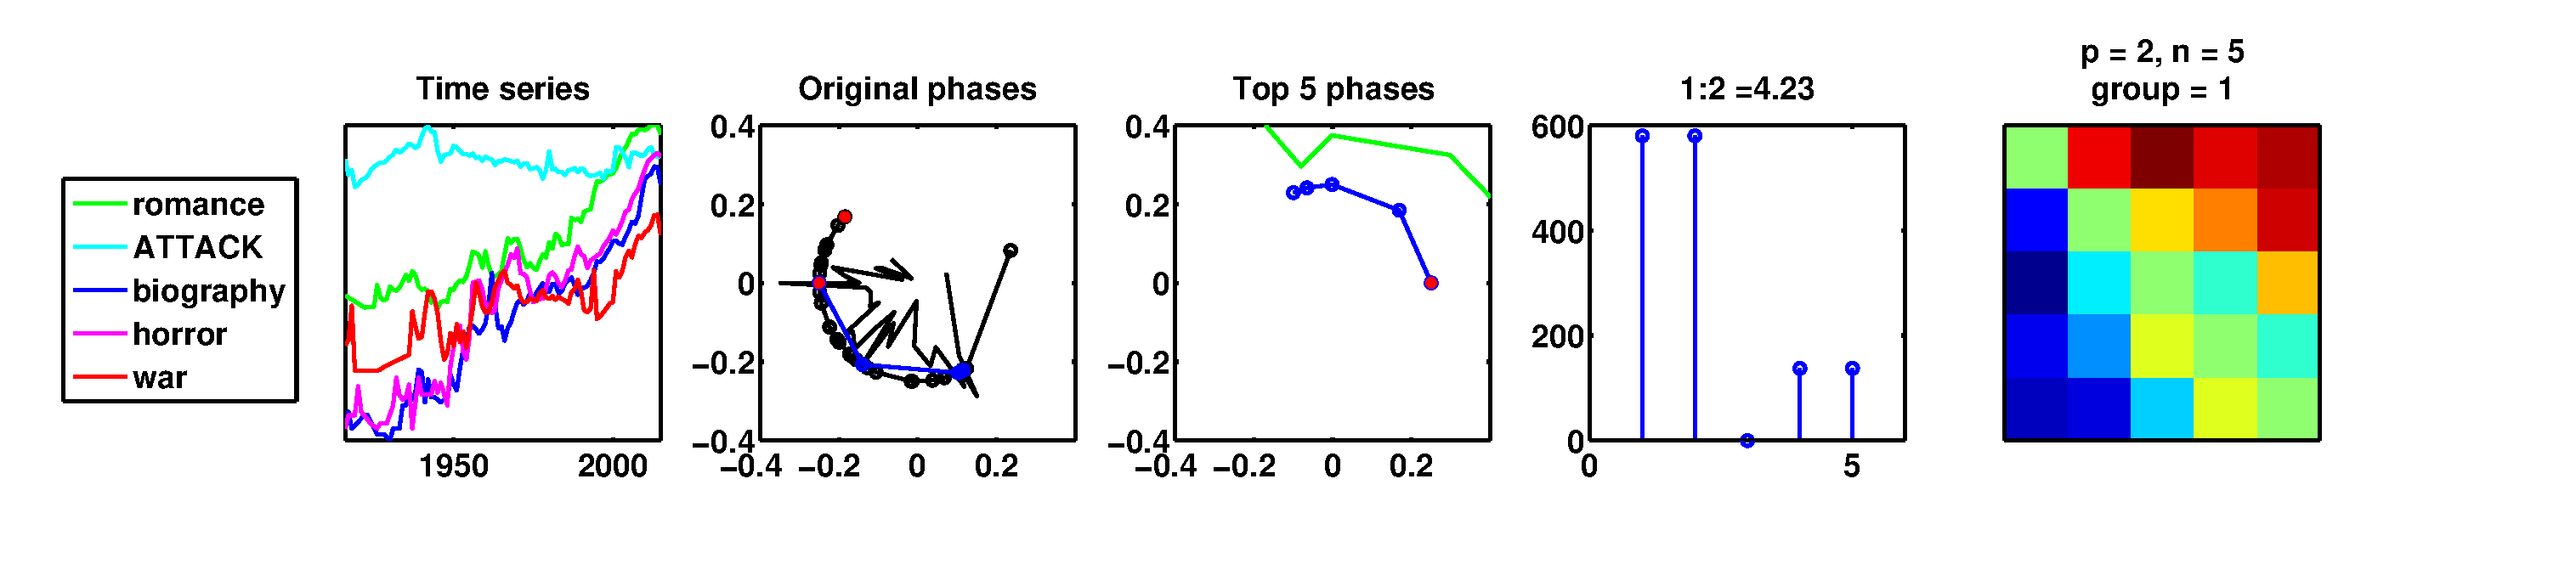
\includegraphics[trim = 0 0 130 0, clip, width=\textwidth]{pictures/_p2_n5_gp1.eps}
\caption{Results with n=5.}
\end{figure}

In each figure, the first subplot on the left shows the original traces (log scale) of the $n$ categories. The next subplot shows the original phase plot in black with the final $n$ categories highlighted in blue with the new ordering. Mostly the ordering from the initial analysis is preserved, but there are a few places (\verb|p=1|, \verb|n=5|, \verb|group=2|, for example) where if two categories were initially close together, they get exchanged in the final ordering. The final three plots are the same thing that we have been looking at all along for the subset of $n$ categories. Note that for the eigenvector ratio label on subplot 4, I the label says 1:2, which is actually 1:3 since the eigenvalues are complex conjugates so 1 and 2 have the same absolute value. If the third eigenvector was equal to 0 (odd man out), then I took the ratio of the first to the next non-zero (first:fourth technically).

\subsection{Impressions}
\begin{itemize}
\item I like the set of five. It is easy to digest and has high e1:e2 ratios. Until I have some reason to do otherwise,  I'll look at sets of 5.
\item Group 2 is not fantastic. Of the three analyses shown, it has the lowest e1:e2 ratio. I will probably run it anyway when we look at the brain permutations.
\item I would like to cut off the first 40 years as before and see what those trends look like.
\end{itemize}

\section{2/6/16}
\subsection{Recent movie data (1955-2015)}
As before, I reduced the movie data to only more recent trends. I learned today that "talkies" started in the 1920's with the first feature length film with synchronized dialogue was released in 1927. This probably explains the leap in production of music and musical films in the late 1920's. It is interesting, however, that in analyzing only more recent trends, 
\begin{itemize}
\item Clusters become quite obvious by looking at the lead matrix;
\item First eigenvalue, group 1 analysis does not wrap around the full cycle anymore;
\item Second eigenvalue ordering has lower e1:e2 ratio with a fuzzier lead matrix and now wraps around a full cycle.
\end{itemize}

Observe the following results on only the recent data.

\begin{figure}[H]
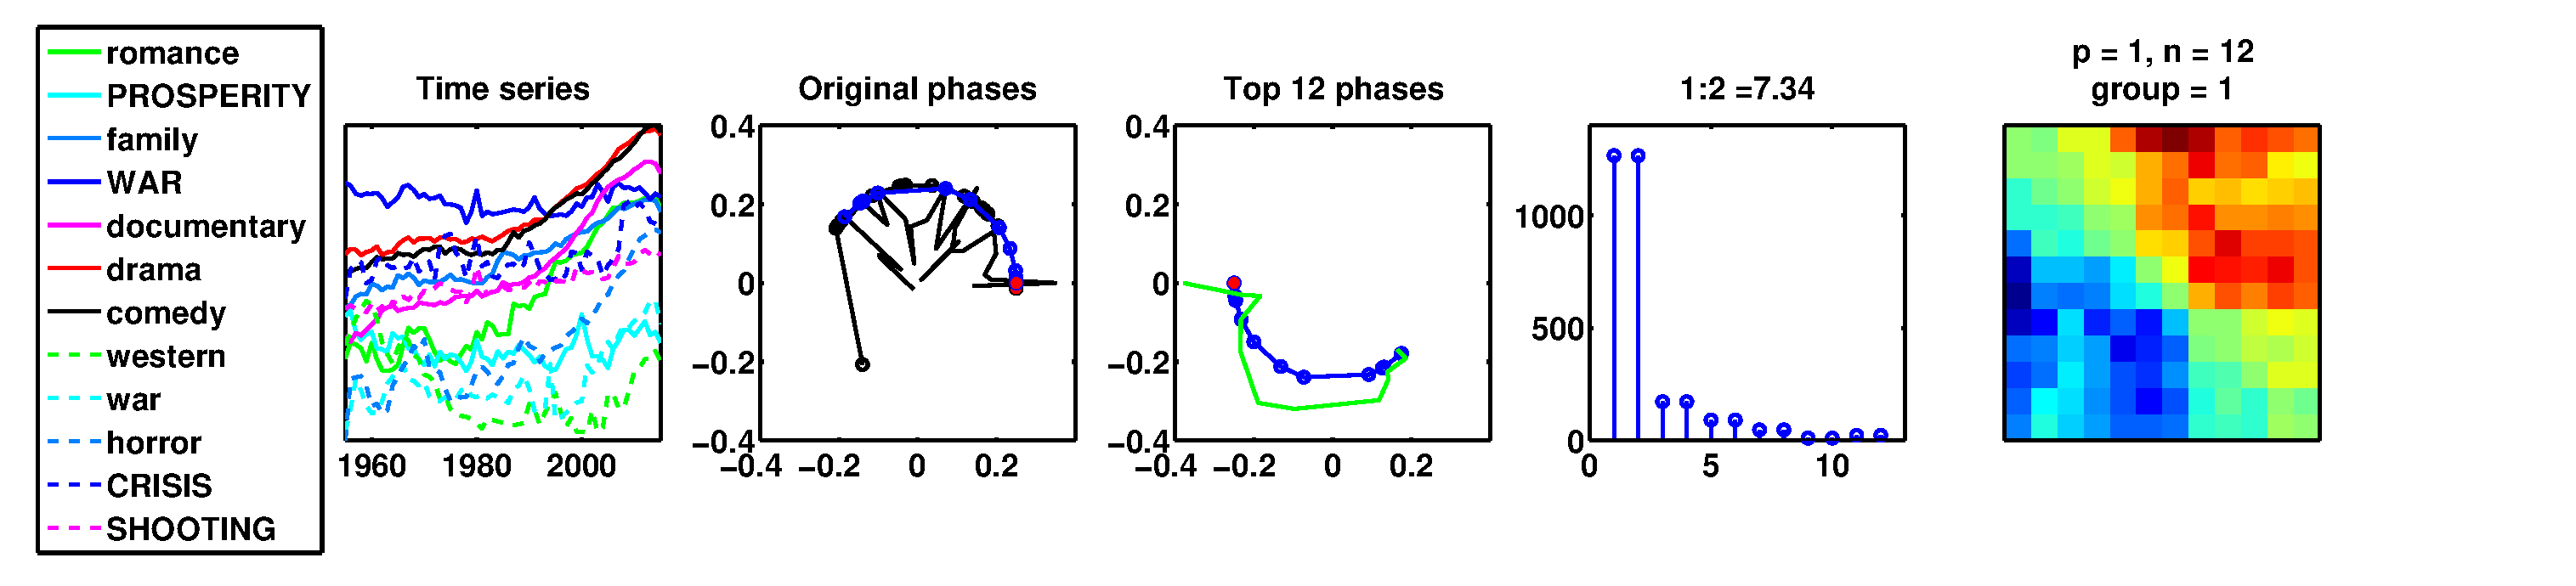
\includegraphics[trim = 0 0 130 0, clip, width=\textwidth]{pictures/movie_word_data_1955-2015_p1_n12_gp1.eps}
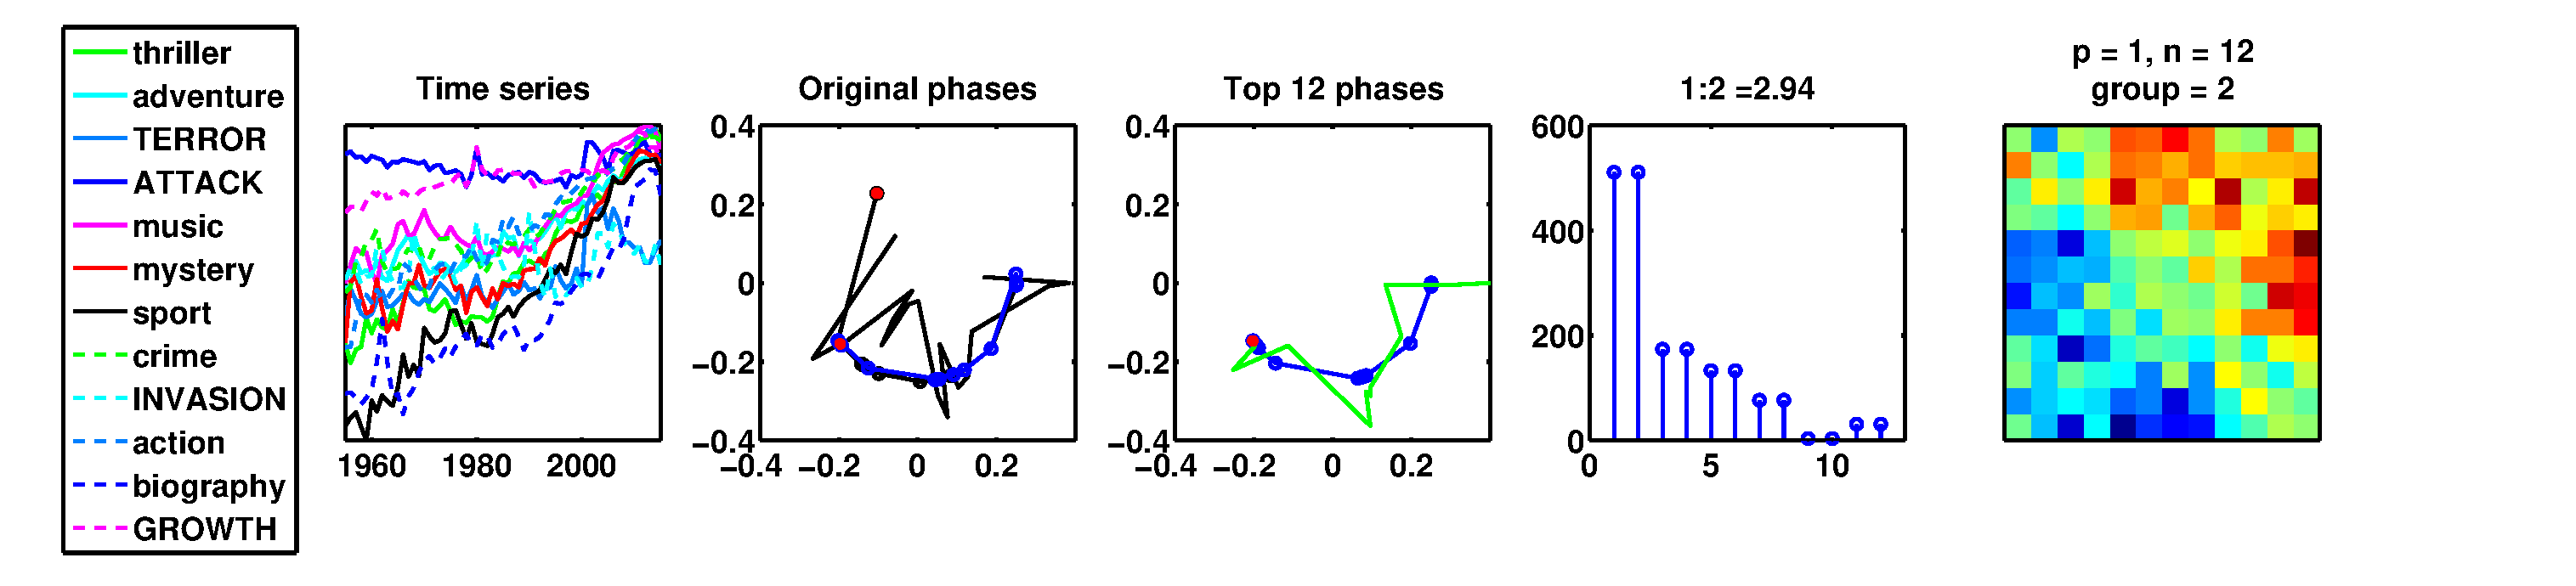
\includegraphics[trim = 0 0 130 0, clip, width=\textwidth]{pictures/movie_word_data_1955-2015_p1_n12_gp2.eps}
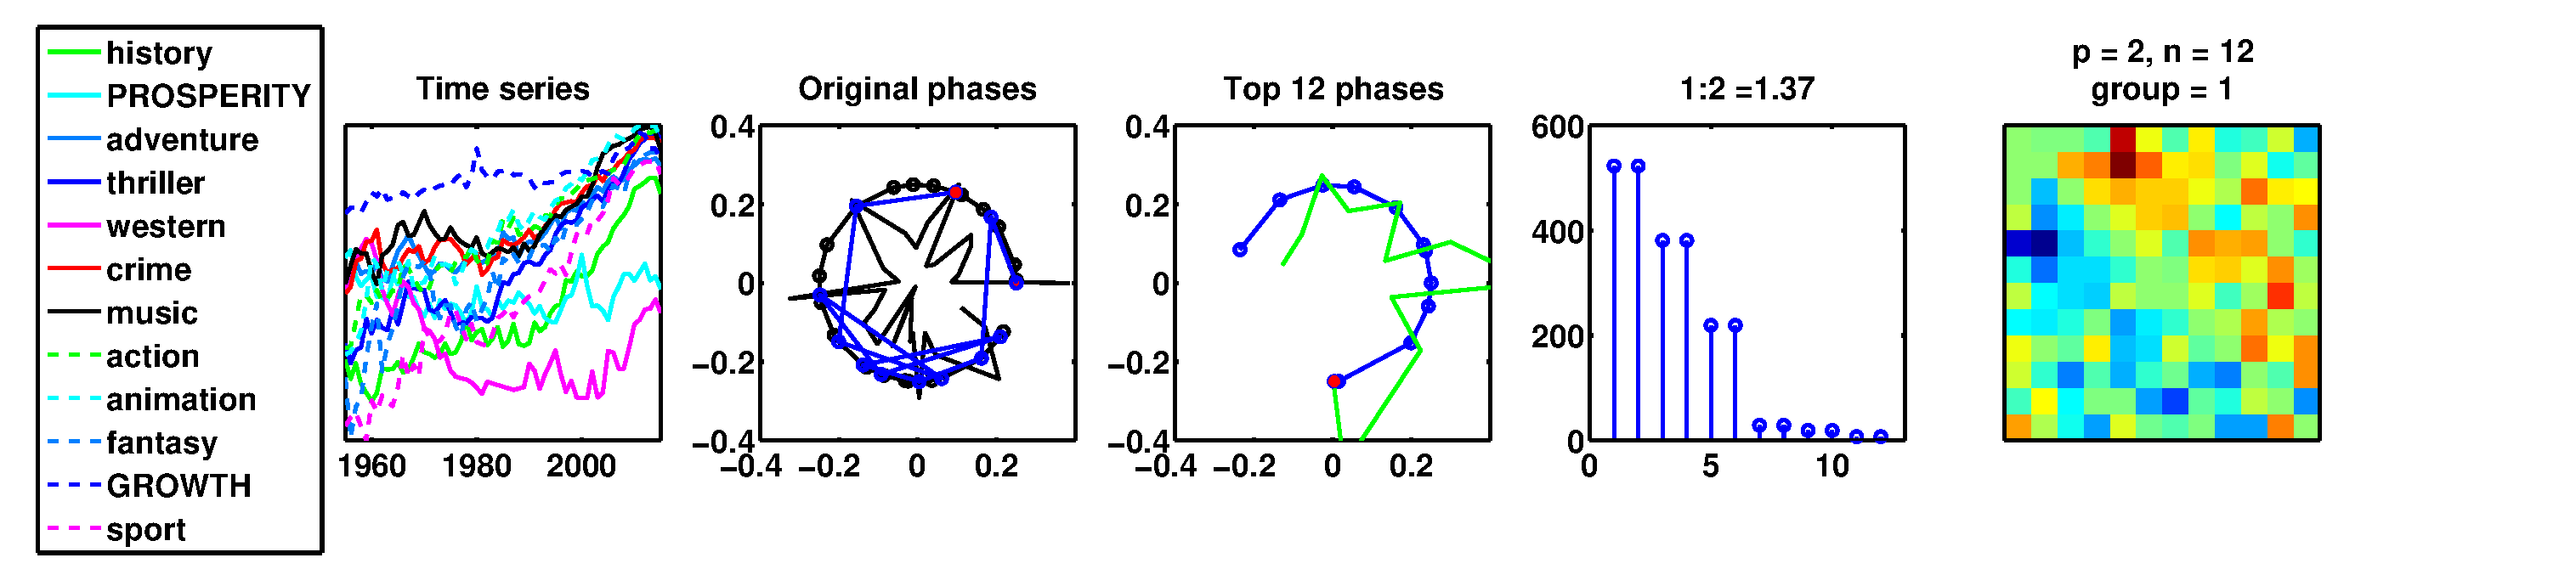
\includegraphics[trim = 0 0 130 0, clip, width=\textwidth]{pictures/movie_word_data_1955-2015_p2_n12_gp1.eps}
\caption{Results with n=12.}
\end{figure}

\begin{figure}[H]
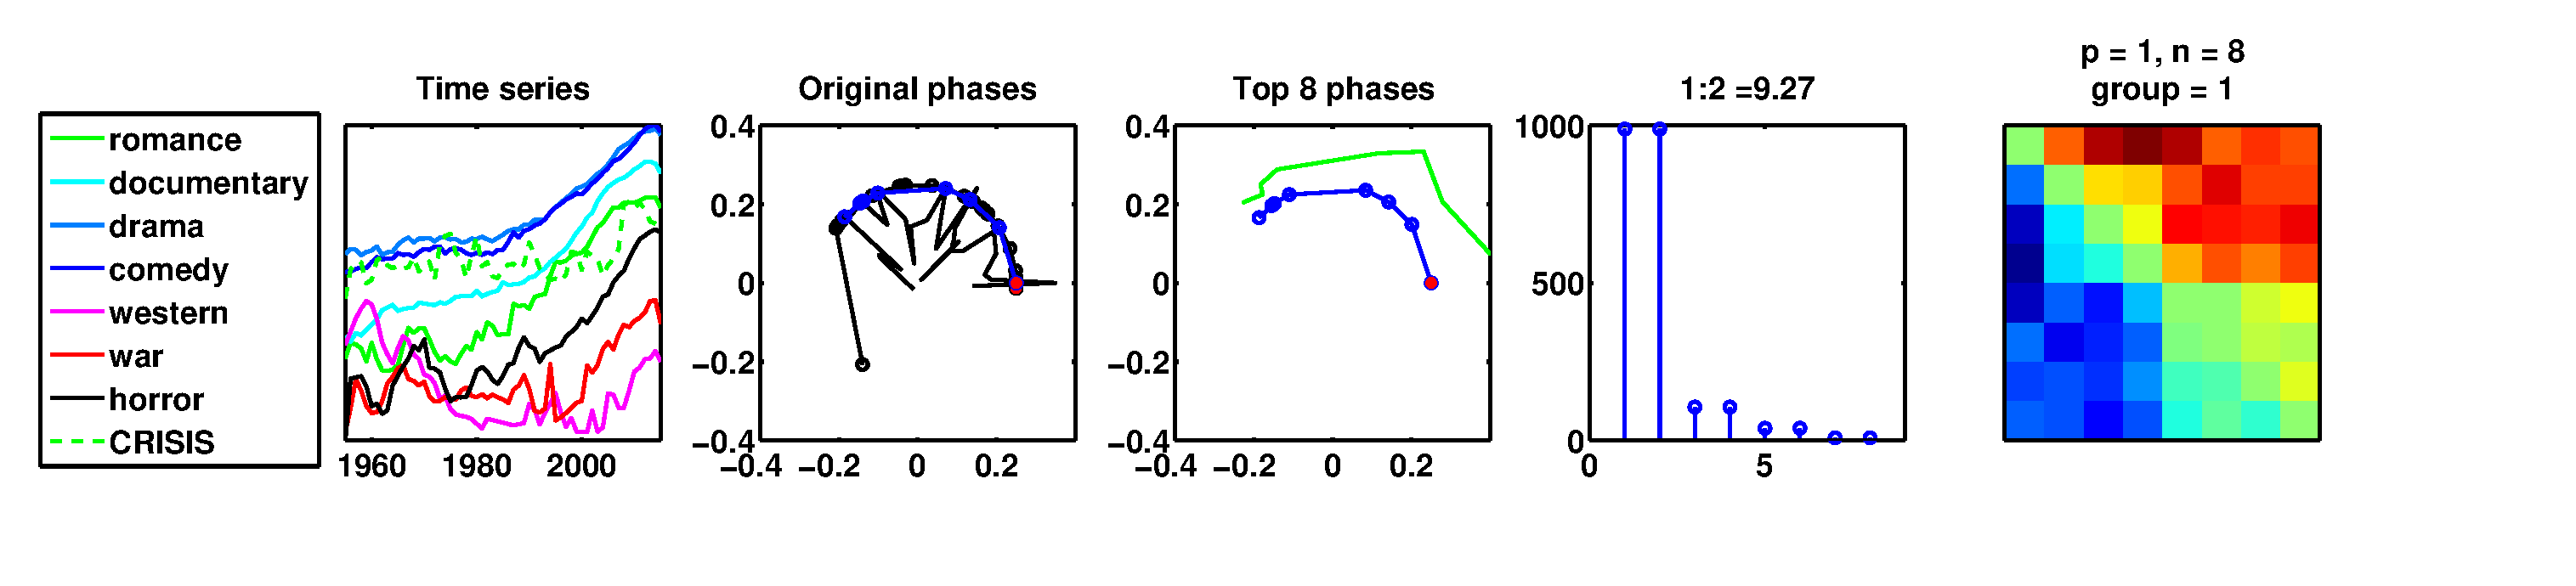
\includegraphics[trim = 0 0 130 0, clip, width=\textwidth]{pictures/movie_word_data_1955-2015_p1_n8_gp1.eps}
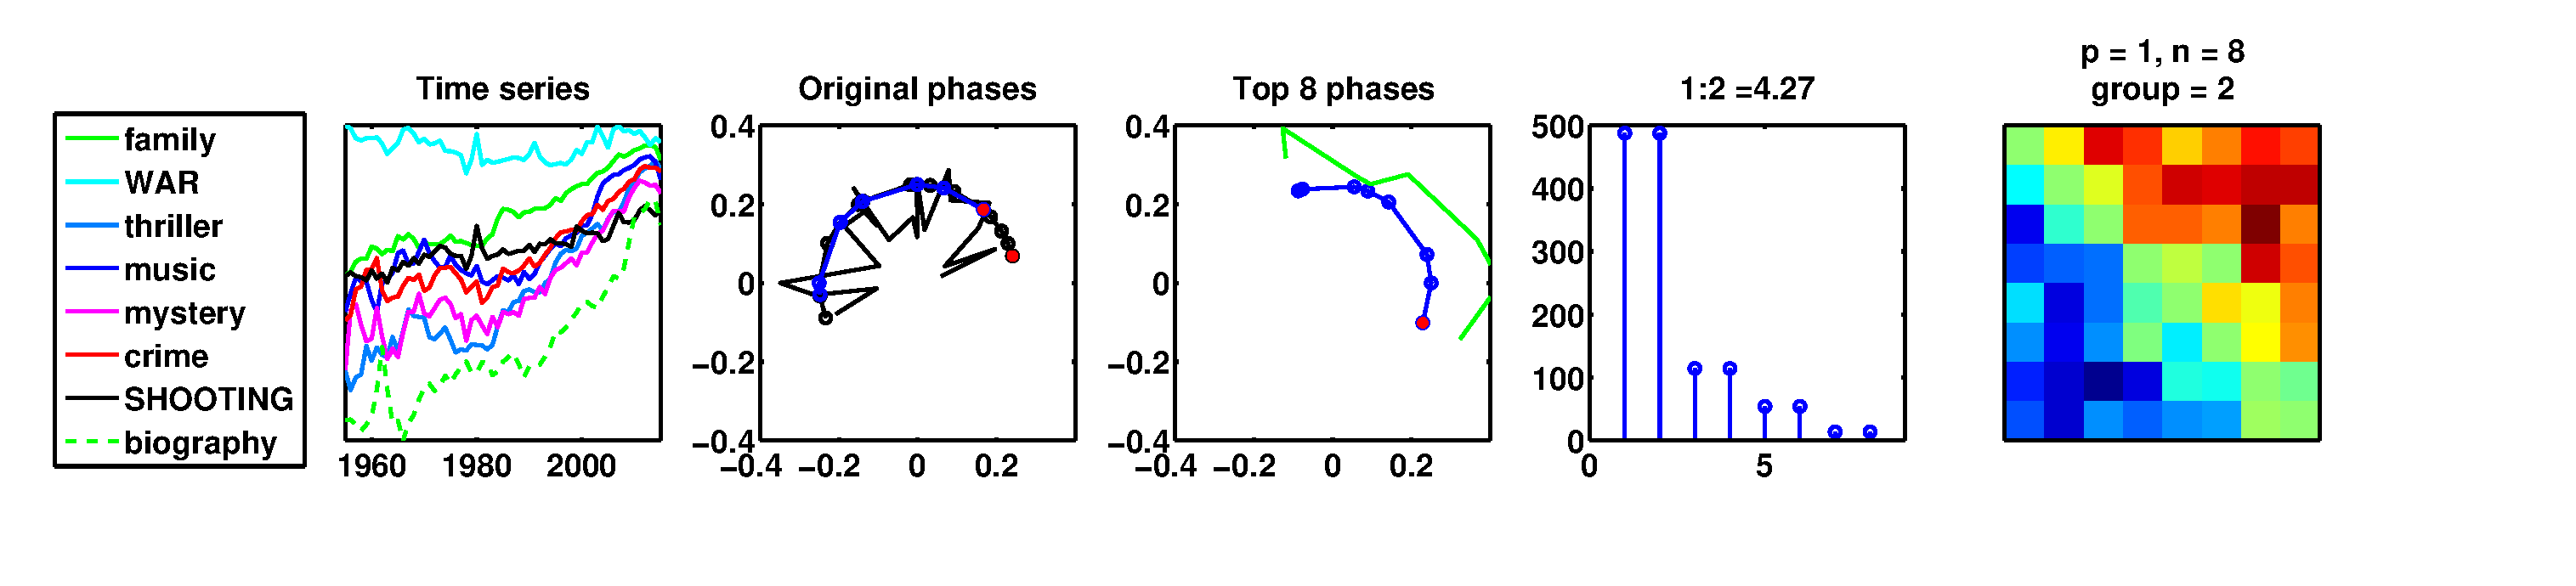
\includegraphics[trim = 0 0 130 0, clip, width=\textwidth]{pictures/movie_word_data_1955-2015_p1_n8_gp2.eps}
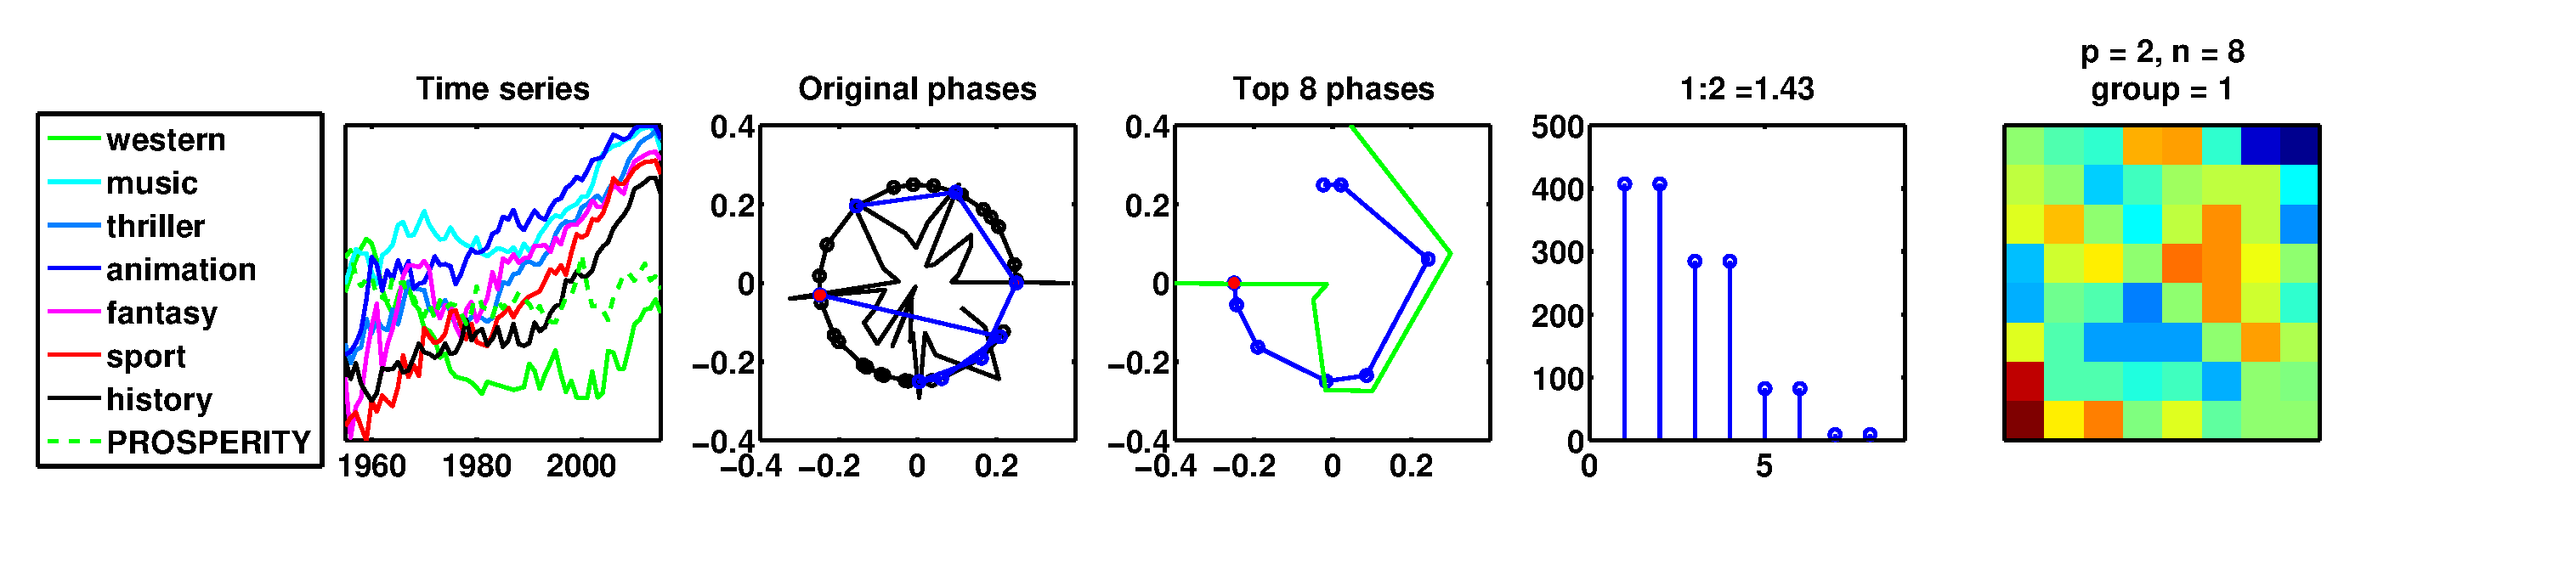
\includegraphics[trim = 0 0 130 0, clip, width=\textwidth]{pictures/movie_word_data_1955-2015_p2_n8_gp1.eps}
\caption{Results with n=12.}
\end{figure}

\begin{figure}[H]
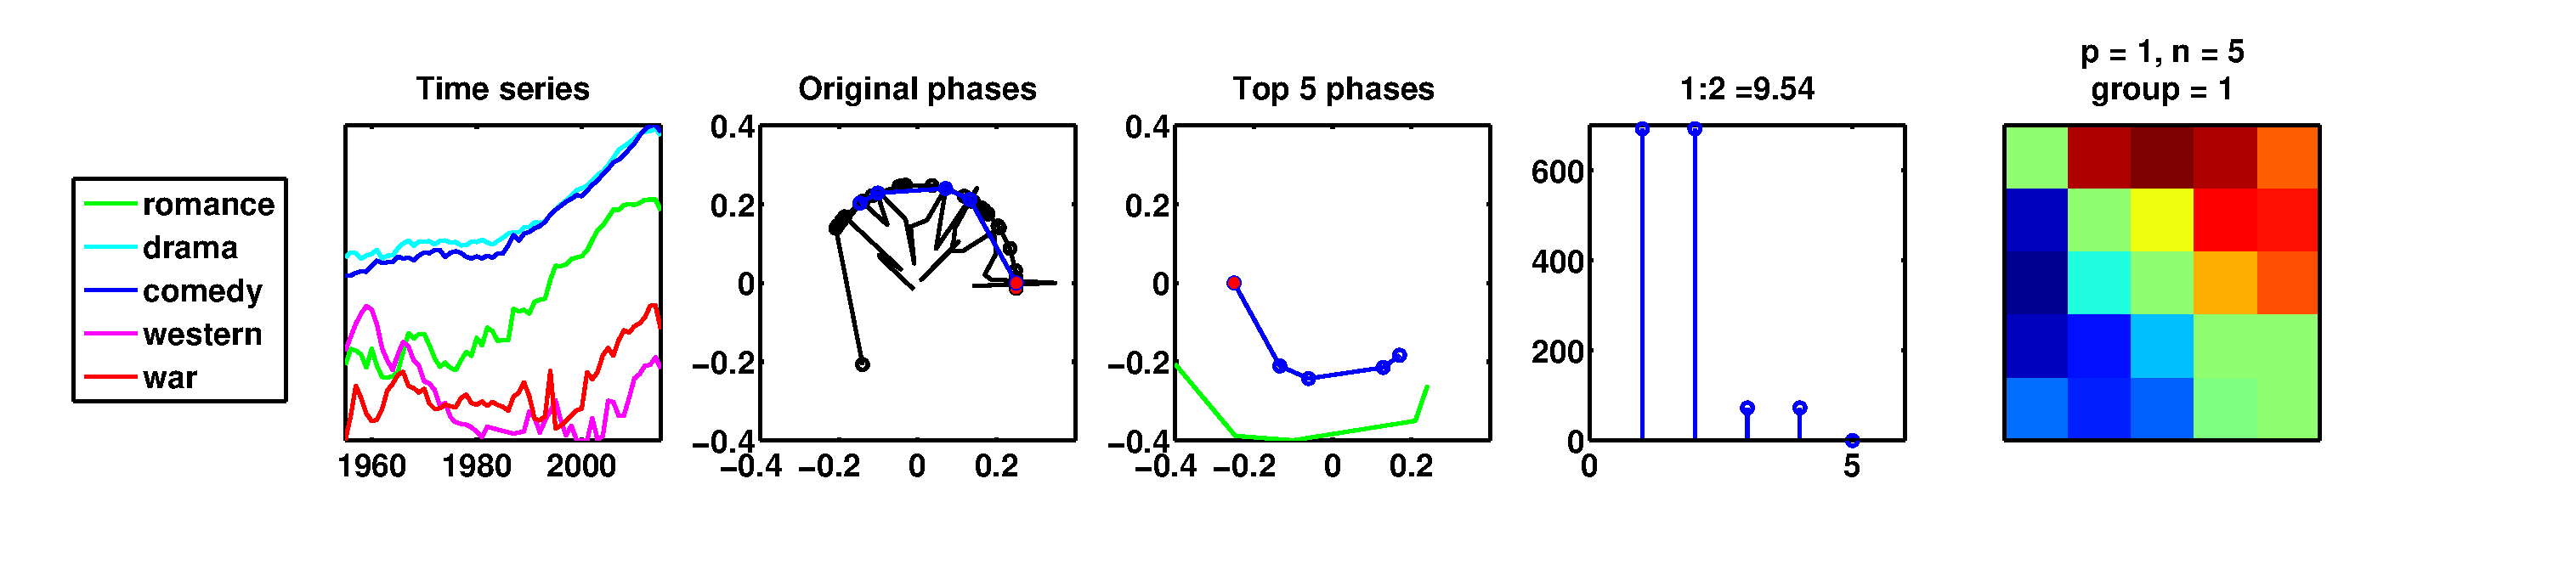
\includegraphics[trim = 0 0 130 0, clip, width=\textwidth]{pictures/movie_word_data_1955-2015_p1_n5_gp1.eps}
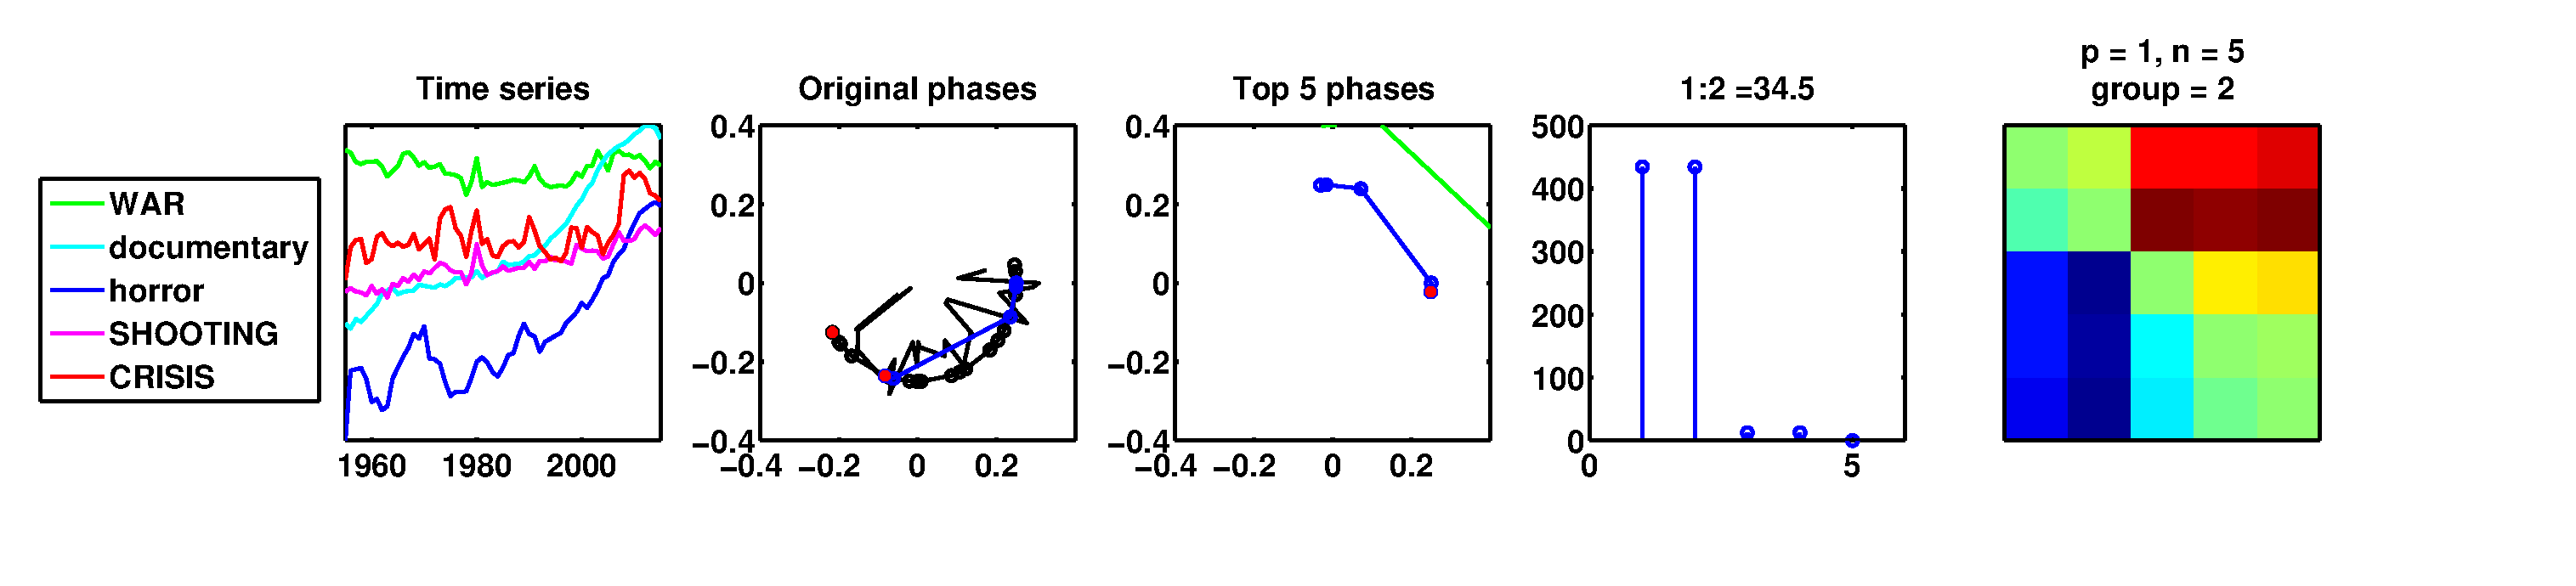
\includegraphics[trim = 0 0 130 0, clip, width=\textwidth]{pictures/movie_word_data_1955-2015_p1_n5_gp2.eps}
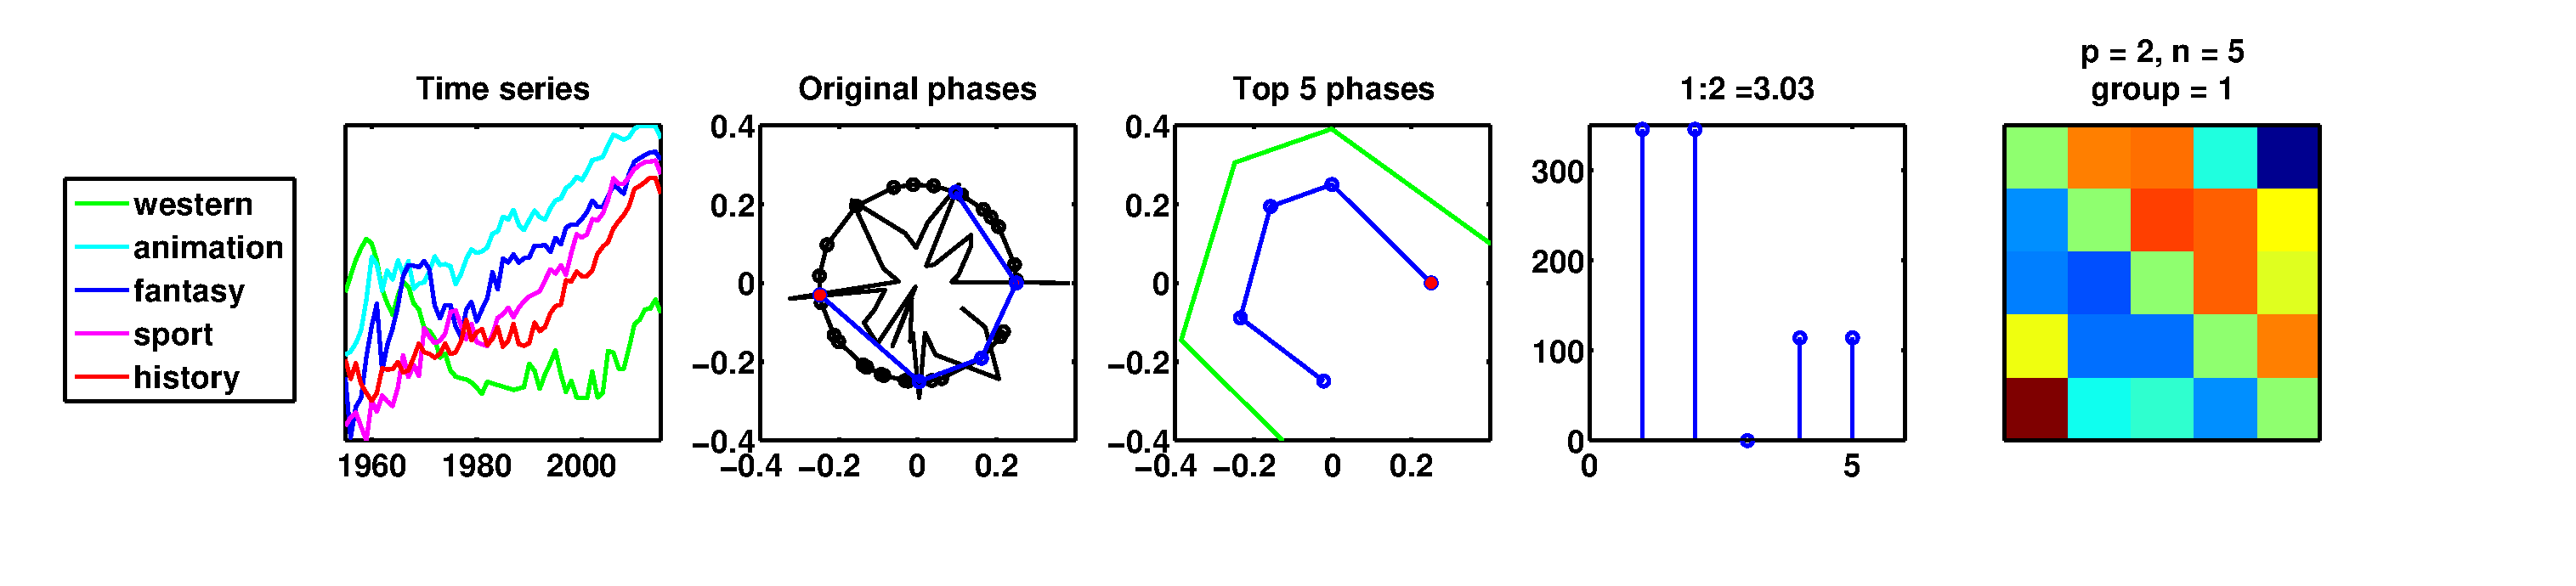
\includegraphics[trim = 0 0 130 0, clip, width=\textwidth]{pictures/movie_word_data_1955-2015_p2_n5_gp1.eps}
\caption{Results with n=12.}
\end{figure}

\section{2/16/16}
\begin{figure}
\label{fig:top12hist}
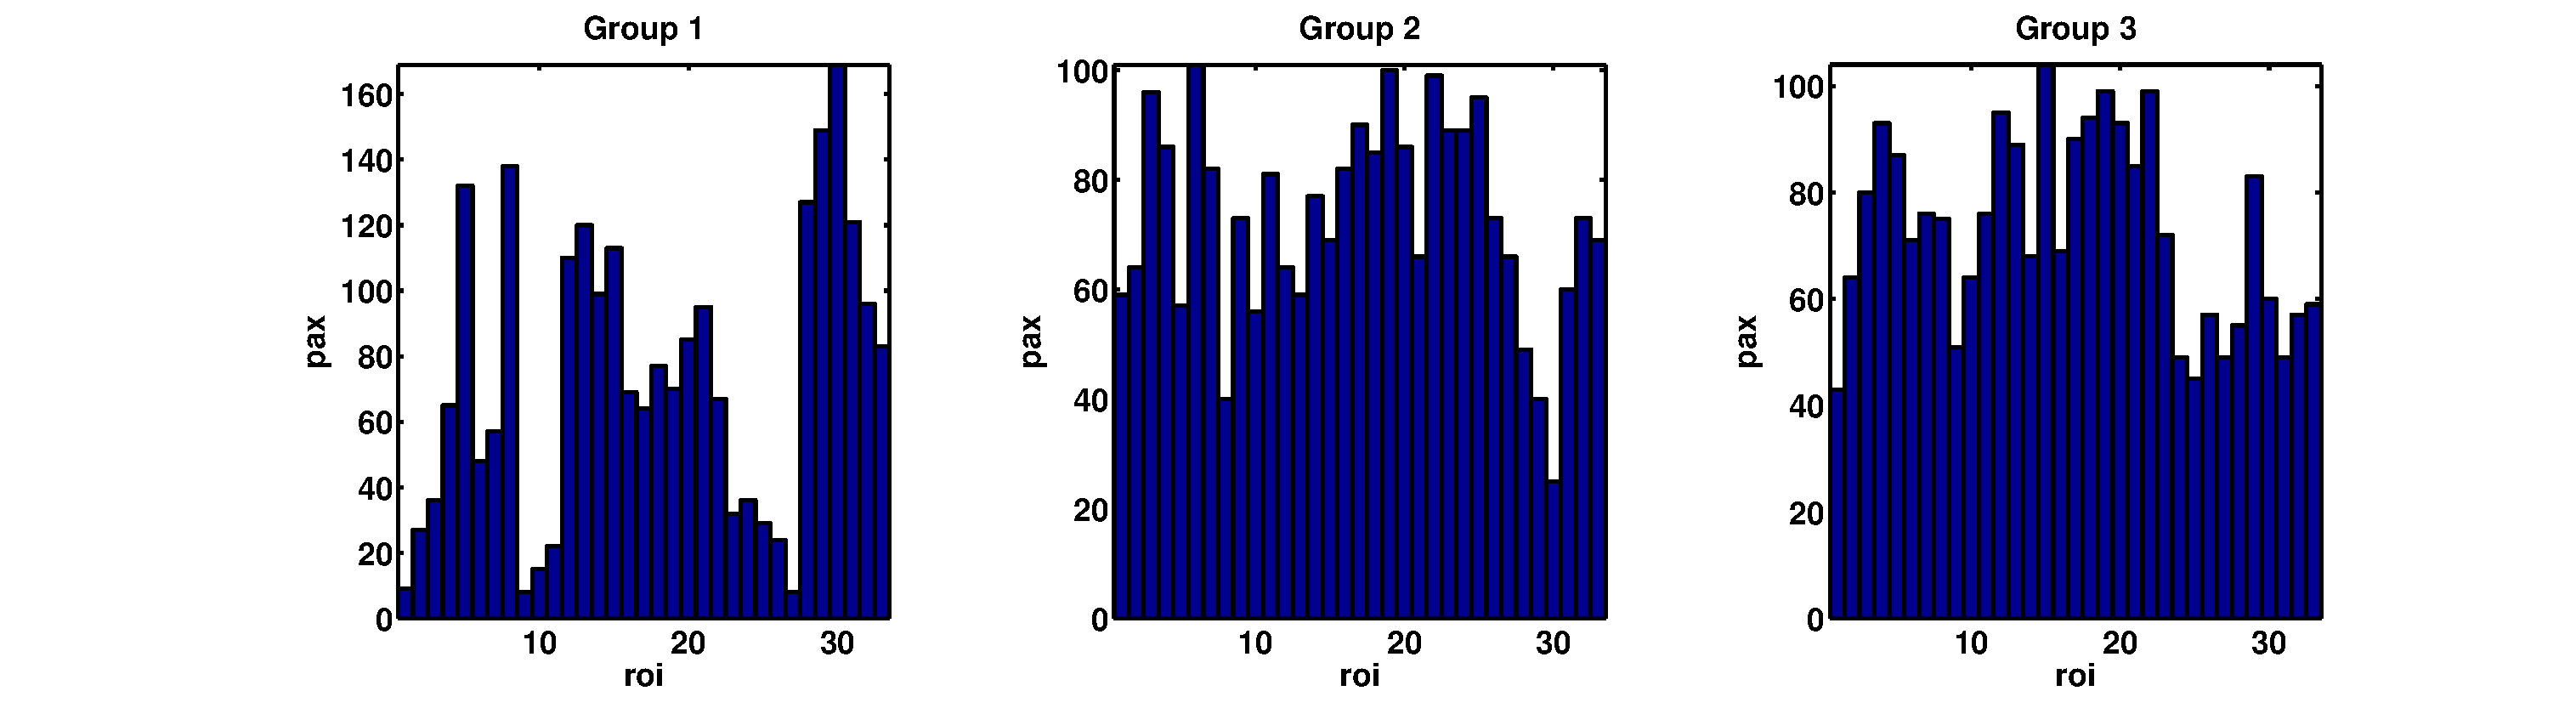
\includegraphics[trim = 50 0 50 0, clip, width = \textwidth]{pictures/refine_cyclicity_output_n12.eps}
\caption{Histogram of top 12 regions (highest phase magnitude) for 200 HCP subjects. Group 1 shows the results for the top 12 regions using the first eigenvector; Group 2 shows the results for the top 12 regions using first eigenvector from the subset of all regions minus those in Group 1; Group 3 shows the results for the top 12 regions using the second eigenvector.}
\end{figure}
This week we analyzed the data from the 200 HCP subjects and compared the top $n$ regions in each subject ($n \in \{5,8,12\}$). We then summarized the results by histogramming the number of appearances of each roi for all 200 of the subjects. The results for $n=12$ are shown in ~\ref{fig:top12hist}. These results were then used to generate the following groups of 10 ``champions.''

\begin{minipage}{.5\textwidth}
\begin{tabular}{ll}
\multicolumn{2}{c}{Group 1}\\
\hline
30 & l cuneus\\
29 & l primary visual cortex\\
8 & l primary auditory cortex\\
5 & precuneus*\\
28 & r primary visual cortex\\
31 & r cuneus\\
13 & l ventral intraparietal sulcus**\\
15 & l posterior intraparietal sulc**\\
12 & r ventral intraparietal sulcus**\\
14 & r posterior intraparietal sulc**\\
\end{tabular}
\end{minipage}
\begin{minipage}{.5\textwidth}
\begin{tabular}{ll}
\multicolumn{2}{c}{Group 3}\\
\hline
15 & l posterior intraparietal sulc**\\
19 & l superior temporal junction*\\
22 & r mid frontal gyrus*\\
12 & r ventral intraparietal sulcus**\\
18 & r superior temporal junction*\\
4 & posterior cingulate cortex*\\
20 & r superior temporal sulcus*\\
17 & r inferior partietal lobe**\\
13 & l ventral intraparietal sulcus**\\
5 & precuneus*\\
\end{tabular}
\end{minipage}
\vspace{10pt}

Definitely need to do more reading or talk to Fatima and Sara about how these regions are related. Wikipedia gives the following functions (for the less obvious regions):
\begin{itemize}
\item Ventral intraparietal sulcus (VIPS): visual attention and saccadic eye movement
\item Posterior (caudal) IPS: perception of depth from stereopsis
\item Cuneus: involved in basic visual processing
\item Precuneus: involved in loads of stuff including default network and visuospatial processing
\item Superior temporal junction (temporoparietal junction): information processing and perception (right and left do not do exactly the same thing - right is more associated with attention and left with language processing)
\item Middle frontal gyrus: part of prefrontal cortex - executive function including attention and working memory
\item Posterior cingulate: central node in DMN
\item Superior temporal sulcus: social perception - responds more to human stimuli rather than environmental/other object
\item Inferior parietal lobe: perception of emotion and faces, interpretation of sensory input
\end{itemize}

\begin{wrapfigure}{r}{.5\textwidth}
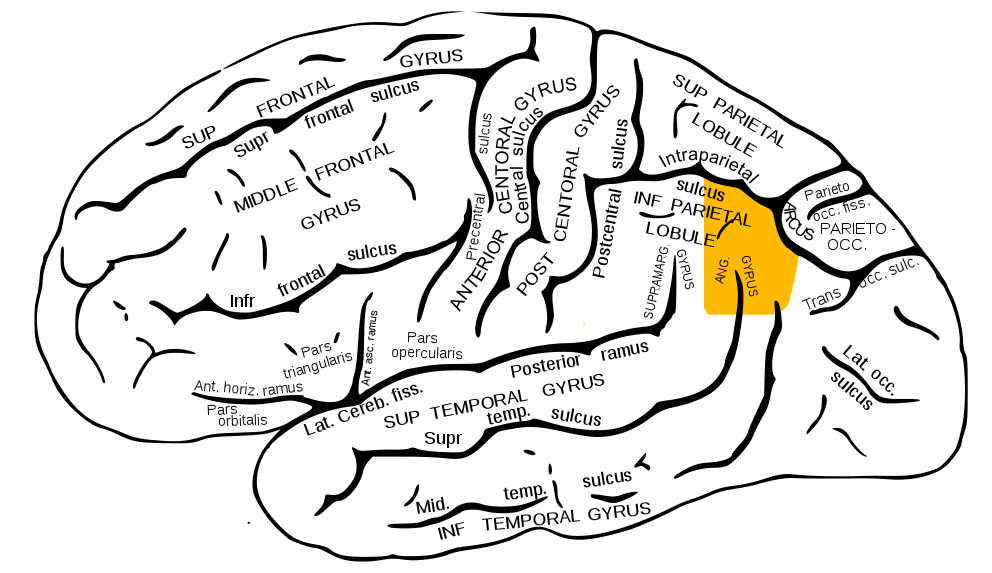
\includegraphics[width=.5\textwidth]{pictures/Gray726_angular_gyrus.png}
\caption{Angular gyrus}
\end{wrapfigure}

Regions marked with `*' are those which are indicated in the DMN. Those marked with `**' surround the angular gyrus, which is also included in the DMN, but is not one of the regions on our list. The acutal DMN regions listed in Wikipedia include
\begin{itemize}
\item PCC \& Precuneus
\item mPFC
\item Angular gyrus
\item TPJ (Dorsomedial subsystem)
\item Lateral temporal cortex (Dorsomedial subsystem)
\end{itemize}
It might be worth looking at the functional regions from Stanford's lab to see if we can reproduce their network associations using the regions they provide.

One interesting observation is the total dominance of the left primary auditory cortex (region 8) in Group 1 compared to the right primary auditory cortex (region 9) which hardly shows up at all. Many other symmetric regions seem to show up in pairs so this contrast is striking.

\subsection{Triples}
\subsubsection{Group 1}
Regions here are numbered as follows:

\vskip 10pt
\begin{center}
\begin{tabular}{ll}
1 & l cuneus \\
2 & l primary visual cortex \\
3 & l primary auditory cortex \\
4 & precuneus \\
5 & r primary visual cortex \\
6 & r cuneus \\
7 & l ventral intraparietal sulcus \\
8 & l posterior intraparietal sulc \\
9 & r ventral intraparietal sulcus \\
10 & r posterior intraparietal sulc \\
\end{tabular}
\end{center}
\vskip 10pt

Analyzing the triples for Group 1 (without correcting for cyclicity) yields the following cycles which are present in at least a third of the subjects (if the cycles are random we might expect any given cycle to be present in 1/6 of the subjects):

\begin{minipage}{.3\textwidth}
\begin{tabular}{ll}
(3,2,1) & 84 \\
(3,4,1) & 70 \\
(3,5,1) & 99 \\
(3,6,1) & 96 \\
(3,7,1) & 87 \\
(9,7,1) & 67 \\
(3,8,1) & 85 \\
(3,9,1) & 94 \\
(3,10,1) & 89 \\
(3,5,2) & 83 \\
(3,6,2) & 87 \\
(3,8,2) & 68 \\
(3,9,2) & 79 \\
(3,10,2) & 78 \\
(3,1,4) & 72 \\
(3,2,4) & 98 \\
(3,5,4) & 105 \\
\end{tabular}
\end{minipage}
\begin{minipage}{.3\textwidth}
\begin{tabular}{ll}
(3,6,4) & 109 \\
(9,6,4) & 71 \\
(3,7,4) & 75 \\
(3,8,4) & 109 \\
(6,8,4) & 73 \\
(9,8,4) & 76 \\
(3,9,4) & 105 \\
(3,10,4) & 110 \\
(9,10,4) & 68 \\
(3,2,5) & 75 \\
(3,6,5) & 86 \\
(3,8,5) & 79 \\
(3,9,5) & 88 \\
(3,10,5) & 86 \\
(3,9,6) & 73 \\
(3,10,6) & 67 \\
\end{tabular}
\end{minipage}
\begin{minipage}{.3\textwidth}
\begin{tabular}{ll}
(3,2,7) & 90 \\
(3,4,7) & 80 \\
(3,5,7) & 100 \\
(3,6,7) & 105 \\
(3,8,7) & 91 \\
(3,9,7) & 116 \\
(3,10,7) & 96 \\
(3,2,8) & 71 \\
(3,5,8) & 72 \\
(3,6,8) & 78 \\
(3,9,8) & 81 \\
(3,10,8) & 72 \\
(3,5,10) & 71 \\
(3,6,10) & 76 \\
(3,8,10) & 72 \\
(3,9,10) & 82 \\
\end{tabular}
\end{minipage}
\vskip 10pt

Worth noting from this is the fact that region 3 (lPAC) nearly always shows up first. After that, however, the order of the subsequent regions seems to be nearly split. By taking cyclicity into account (reordering cycles so that the lowest index always appears first) we can filter out these cycles and we get the following results that are present in at least 60\% of subjects (again, thinking that if cycles are random then any given cycle should show up in 50\% of subjects):

\vskip 10pt
\begin{center}
\begin{minipage}{.3\textwidth}
\begin{tabular}{ll}
(3,5,4) & 127 \\
(3,6,4) & 130 \\
(3,8,4) & 127 \\
(3,9,4) & 123 \\
(3,10,4) & 127 \\
\end{tabular}
\end{minipage}
\begin{minipage}{.3\textwidth}
\begin{tabular}{ll}
(1,3,5) & 133 \\
(1,3,6) & 129 \\
(1,3,7) & 120 \\
(3,5,7) & 122 \\
(3,6,7) & 125 \\
\end{tabular}
\end{minipage}
\begin{minipage}{.3\textwidth}
\begin{tabular}{ll}
(1,9,7) & 133 \\
(3,9,7) & 137 \\
(1,3,9) & 124 \\
(1,3,10) & 123 \\
\end{tabular}
\end{minipage}
\end{center}
\vskip 10pt

Again, the lPAC shows up in every cycle except for one. Is this an outlier or are the fMRI sounds triggering this whole cycle?

\subsubsection{Group 3}
Regions in this group are numbered as follows: 

\vskip 10pt
\begin{center}
\begin{tabular}{ll}
1 & l posterior intraparietal sulc \\
2 & l superior temporal junction \\
3 & r mid frontal gyrus \\
4 & r ventral intraparietal sulcus \\
5 & r superior temporal junction \\
6 & posterior cingulate cortex \\
7 & r superior temporal sulcus \\
8 & r inferior partietal lobe \\
9 & l ventral intraparietal sulcus \\
10 & precuneus \\
\end{tabular}
\end{center}
\vskip 10pt

First, without normalizing for cyclicity:

\vskip 10pt
\begin{minipage}{.25\textwidth}
\begin{tabular}{ll}
(3,2,1) & 69 \\
(3,5,1) & 72 \\
(3,7,1) & 73 \\
(3,8,1) & 67 \\
(5,8,1) & 69 \\
(3,1,4) & 75 \\
(5,1,4) & 69 \\
(3,2,4) & 70 \\
(5,2,4) & 67 \\
(3,5,4) & 68 \\
(3,7,4) & 69 \\
(3,2,8) & 70 \\
(3,5,8) & 75 \\
(2,1,9) & 78 \\
(3,1,9) & 102 \\
(5,1,9) & 93 \\
(6,1,9) & 78 \\
(7,1,9) & 90 \\
\end{tabular}
\end{minipage}
\begin{minipage}{.25\textwidth}
\begin{tabular}{ll}
(8,1,9) & 72 \\
(3,2,9) & 91 \\
(5,2,9) & 85 \\
(6,2,9) & 75 \\
(7,2,9) & 70 \\
(2,4,9) & 78 \\
(3,4,9) & 94 \\
(5,4,9) & 89 \\
(6,4,9) & 81 \\
(7,4,9) & 92 \\
(8,4,9) & 70 \\
(3,5,9) & 86 \\
(3,6,9) & 81 \\
(3,7,9) & 81 \\
(5,7,9) & 74 \\
(2,8,9) & 68 \\
(3,8,9) & 86 \\
(5,8,9) & 90 \\
\end{tabular}
\end{minipage}
\begin{minipage}{.25\textwidth}
\begin{tabular}{ll}
(7,8,9) & 75 \\
(2,10,9) & 79 \\
(3,10,9) & 82 \\
(5,10,9) & 88 \\
(6,10,9) & 81 \\
(7,10,9) & 85 \\
(8,10,9) & 81 \\
(2,1,10) & 80 \\
(3,1,10) & 109 \\
(4,1,10) & 67 \\
(5,1,10) & 92 \\
(6,1,10) & 76 \\
(7,1,10) & 94 \\
(3,2,10) & 104 \\
(5,2,10) & 89 \\
(6,2,10) & 80 \\
(7,2,10) & 84 \\
\end{tabular}
\end{minipage}
\begin{minipage}{.25\textwidth}
\begin{tabular}{ll}
(3,4,10) & 81 \\
(5,4,10) & 73 \\
(7,4,10) & 74 \\
(3,5,10) & 101 \\
(6,5,10) & 73 \\
(7,5,10) & 78 \\
(2,6,10) & 68 \\
(3,6,10) & 100 \\
(5,6,10) & 78 \\
(7,6,10) & 83 \\
(8,6,10) & 69 \\
(3,7,10) & 94 \\
(5,7,10) & 80 \\
(2,8,10) & 93 \\
(3,8,10) & 112 \\
(5,8,10) & 109 \\
(6,8,10) & 75 \\
(7,8,10) & 98 \\
\end{tabular}
\end{minipage}
\vskip 10pt

The most notable feature in this case is that regions 9 and 10 (lVIPS, precuneus) show up last in most of the cycles.

Taking cyclicity into account:

\vskip 10pt
\begin{center}
\begin{minipage}{.25\textwidth}
\begin{tabular}{ll}
(1,4,3) & 120 \\
(1,9,3) & 130 \\
(1,10,3) & 131 \\
(2,10,3) & 130 \\
(1,9,5) & 123 \\
(4,9,5) & 125 \\
(2,8,6) & 127 \\
(5,8,6) & 126 \\
(1,9,6) & 122 \\
\end{tabular}
\end{minipage}
\begin{minipage}{.25\textwidth}
\begin{tabular}{ll}
(4,9,6) & 129 \\
(1,9,7) & 121 \\
(4,9,7) & 125 \\
(4,9,8) & 120 \\
(3,4,9) & 122 \\
(2,10,9) & 122 \\
(5,10,9) & 123 \\
(6,10,9) & 129 \\
(7,10,9) & 120 \\
\end{tabular}
\end{minipage}
\begin{minipage}{.25\textwidth}
\begin{tabular}{ll}
(8,10,9) & 134 \\
(3,5,10) & 125 \\
(3,6,10) & 123 \\
(2,8,10) & 120 \\
(3,8,10) & 135 \\
(4,8,10) & 124 \\
(5,8,10) & 126 \\
(7,8,10) & 120 \\
\end{tabular}
\end{minipage}
\end{center}
\vskip 10pt

\subsubsection{Eigenvalue Ratios}
\begin{figure}[H]
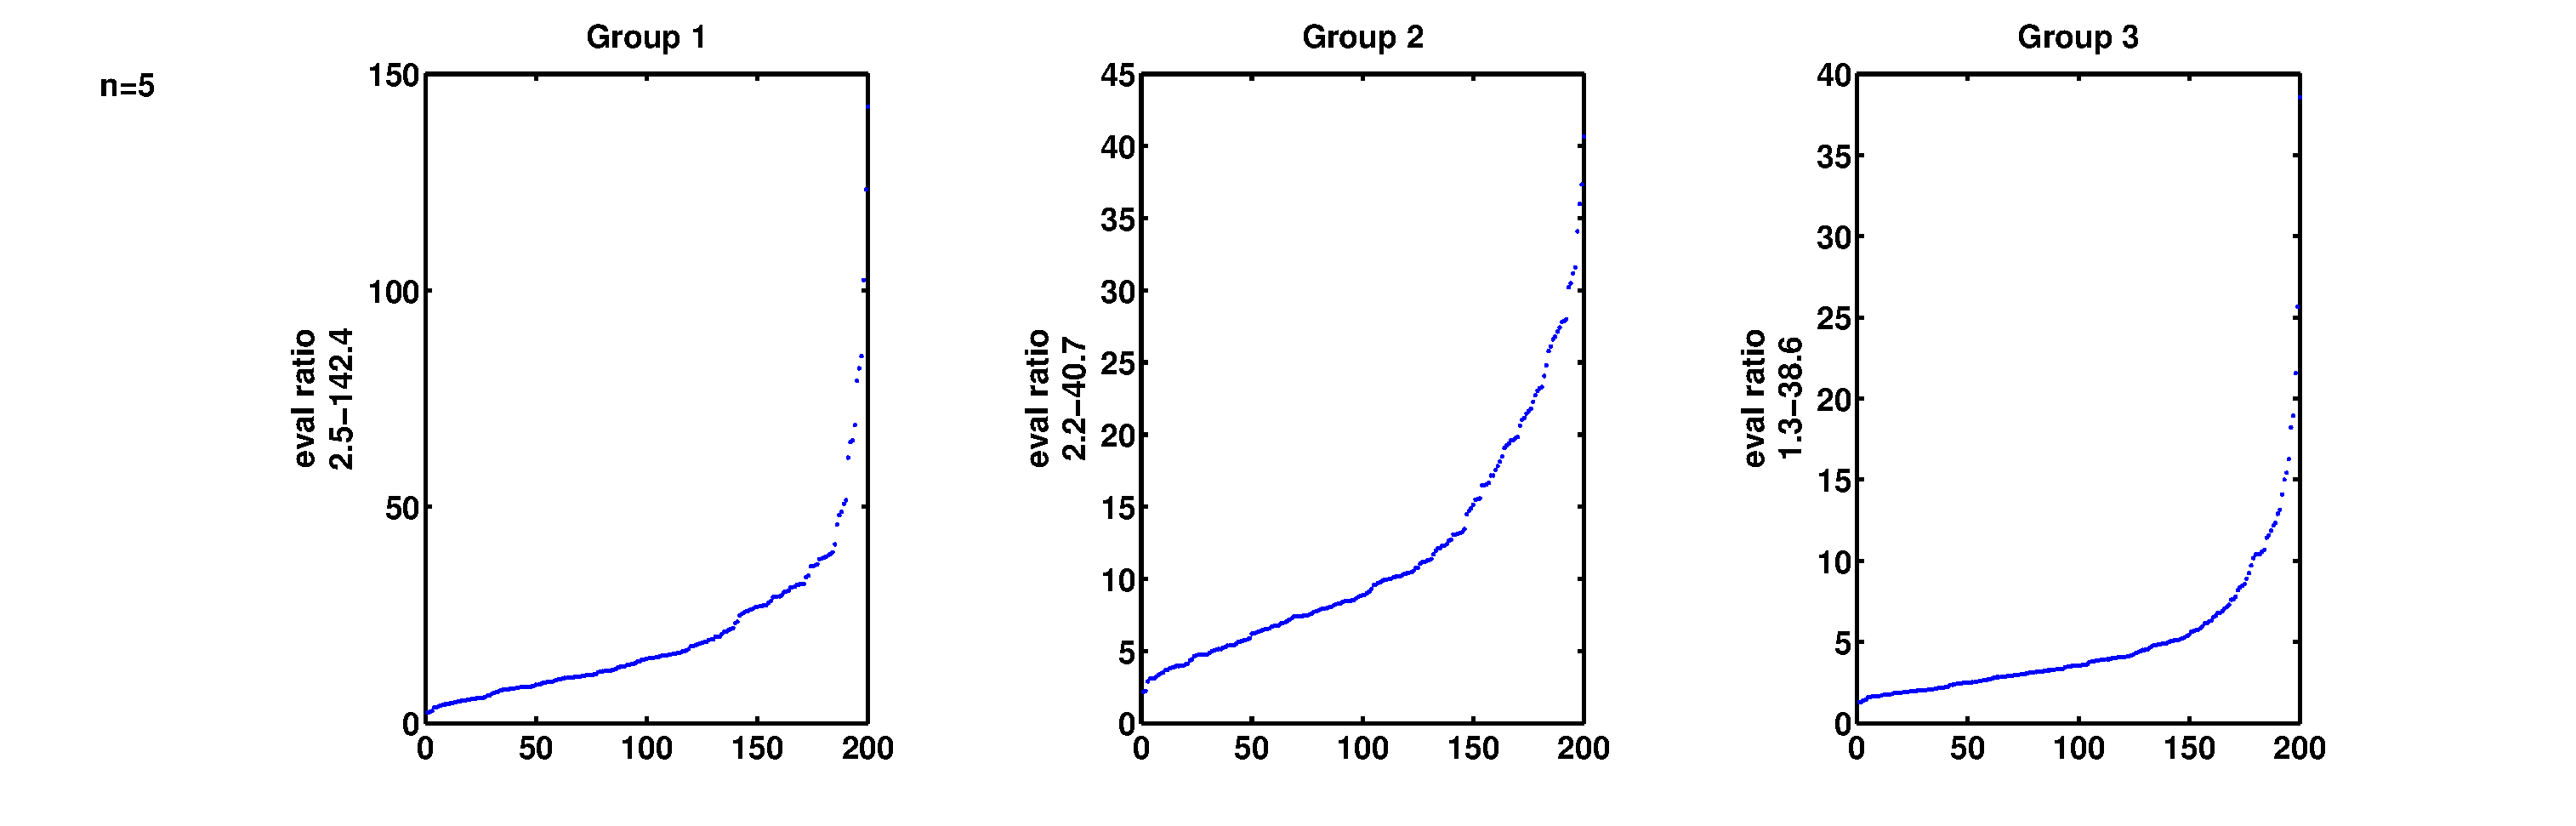
\includegraphics[trim= 20 0 50 0, clip, width=\textwidth]{pictures/refine_cyclicity_output_n5_evals.eps}
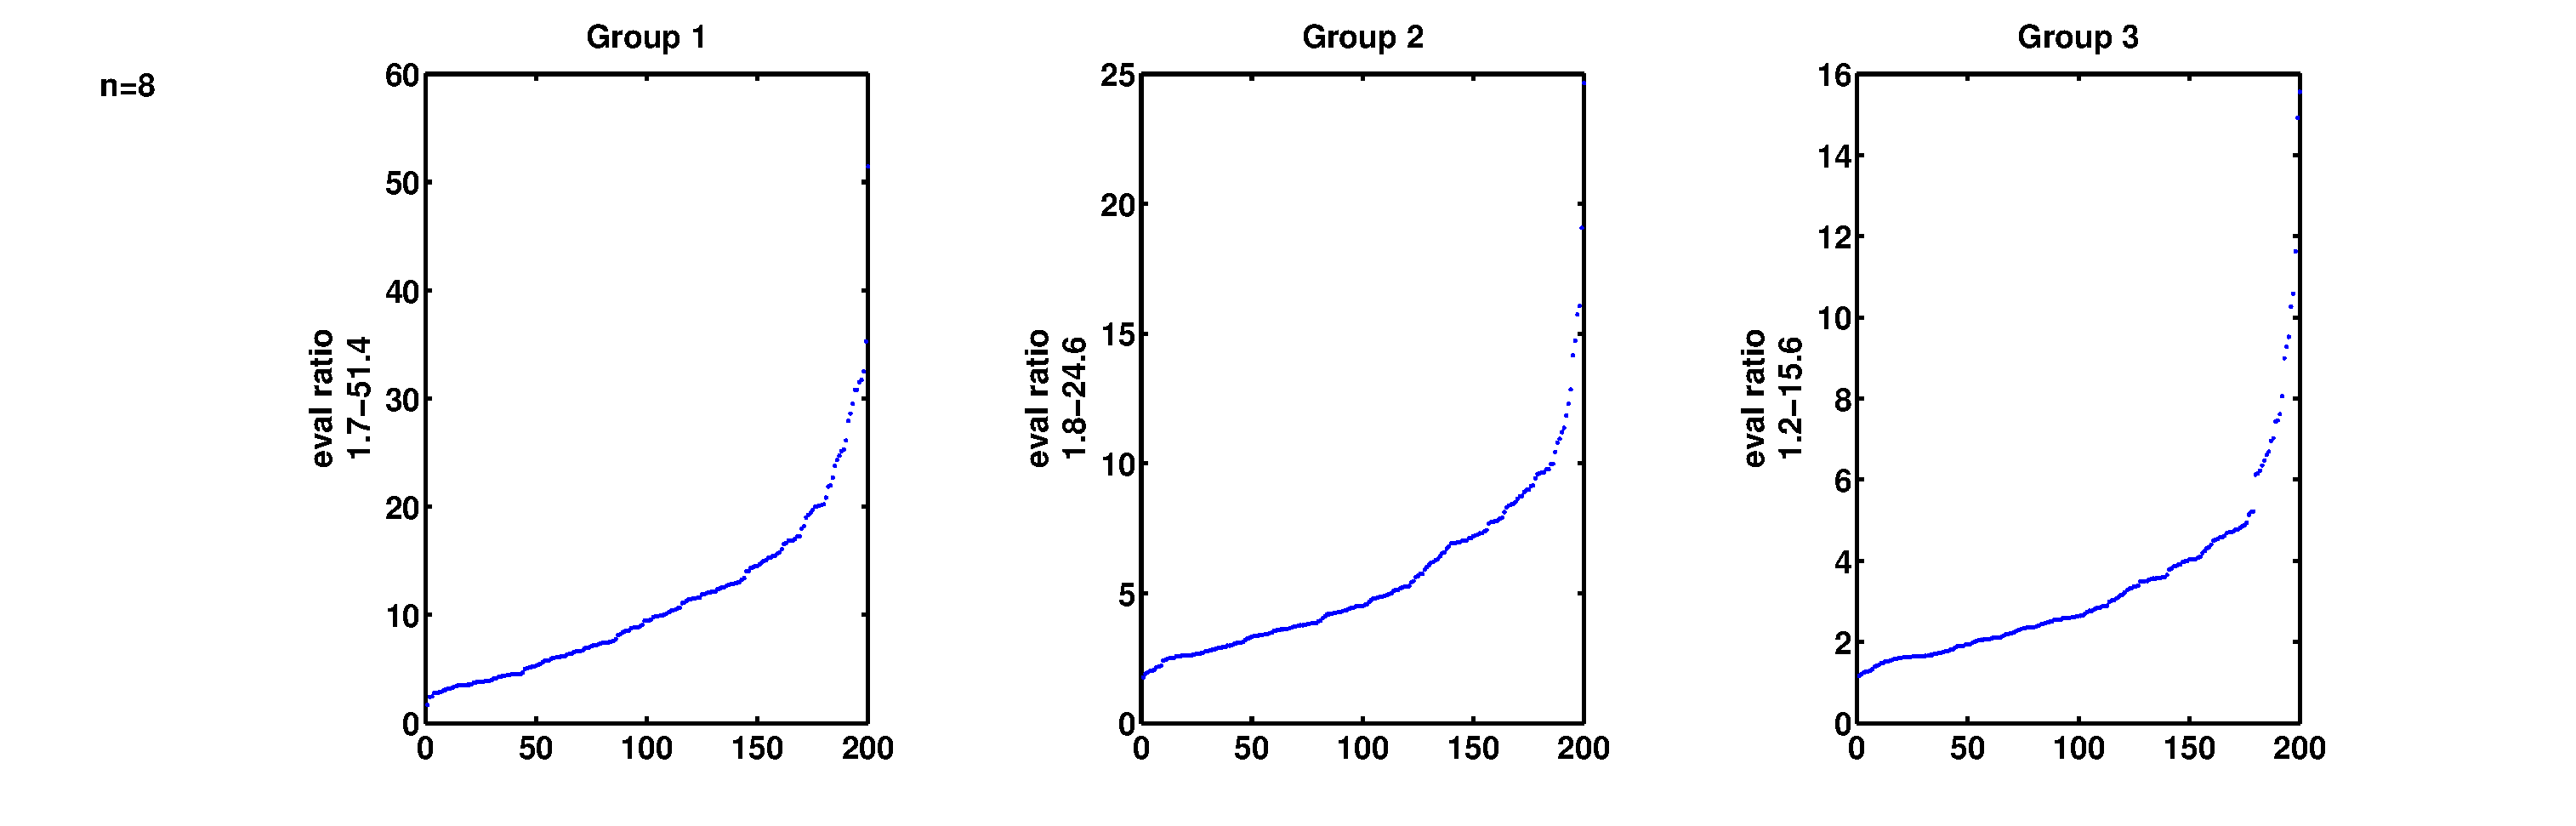
\includegraphics[trim= 20 0 50 0, clip, width=\textwidth]{pictures/refine_cyclicity_output_n8_evals.eps}
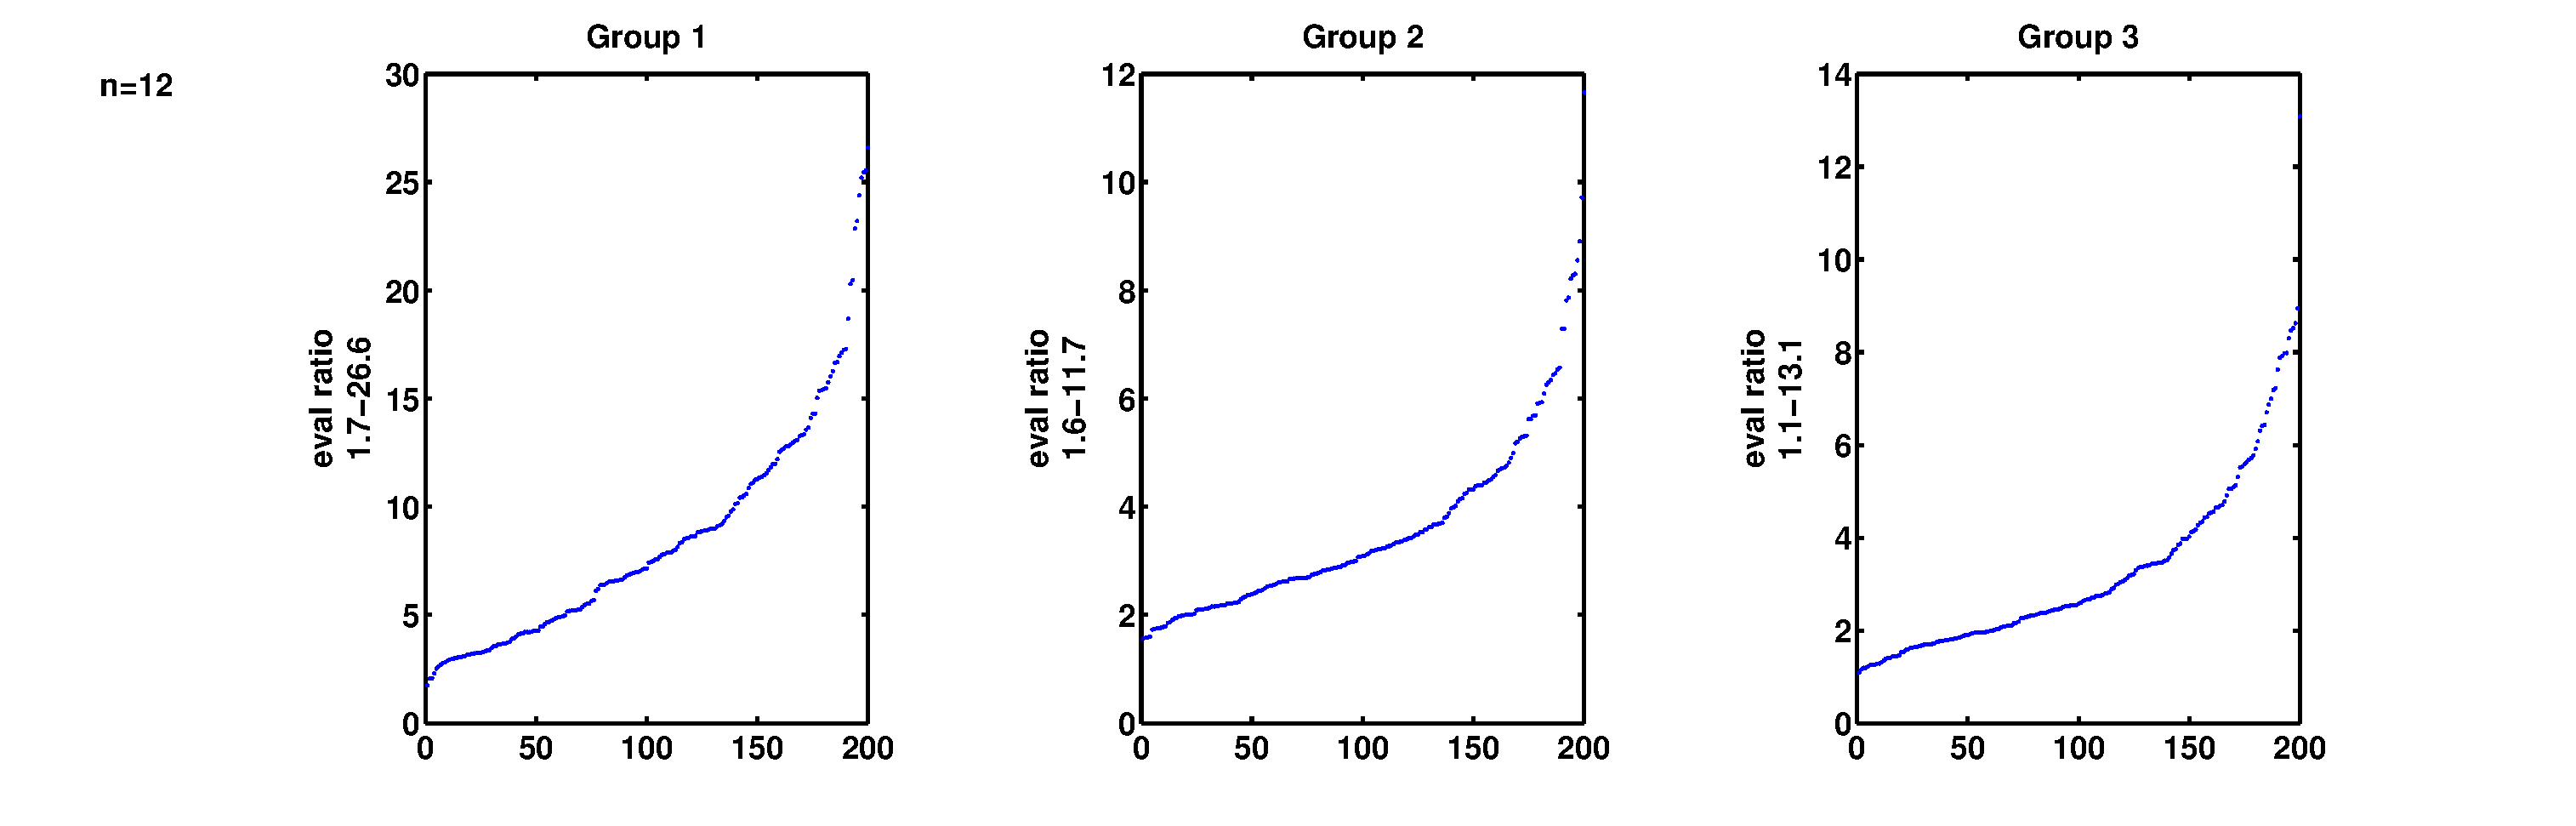
\includegraphics[trim= 20 0 50 0, clip, width=\textwidth]{pictures/refine_cyclicity_output_n12_evals.eps}
\end{figure}

\section{3/8/16}
\begin{figure}
\label{fig:hist}
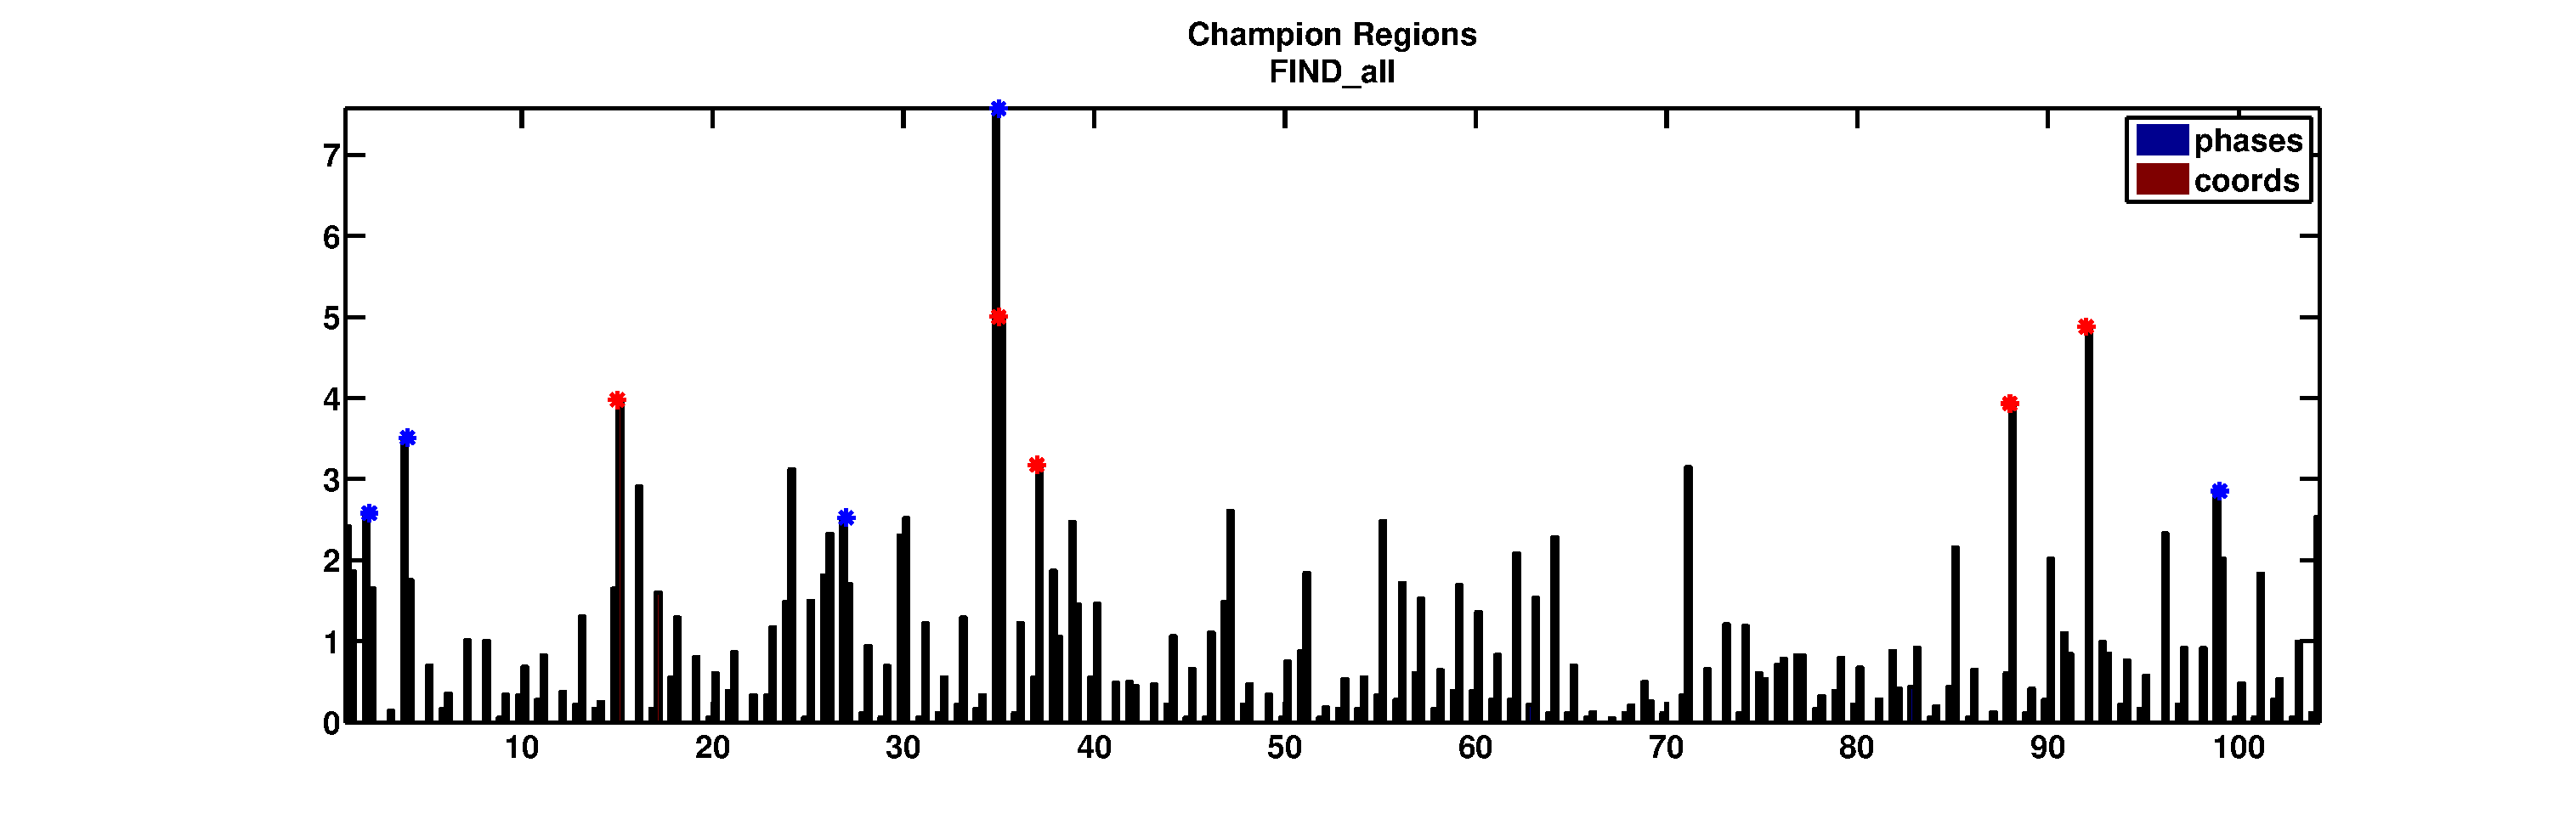
\includegraphics[trim= 150 0 130 0, clip, width = \textwidth]{pictures/hist_n5_FIND_all.eps}
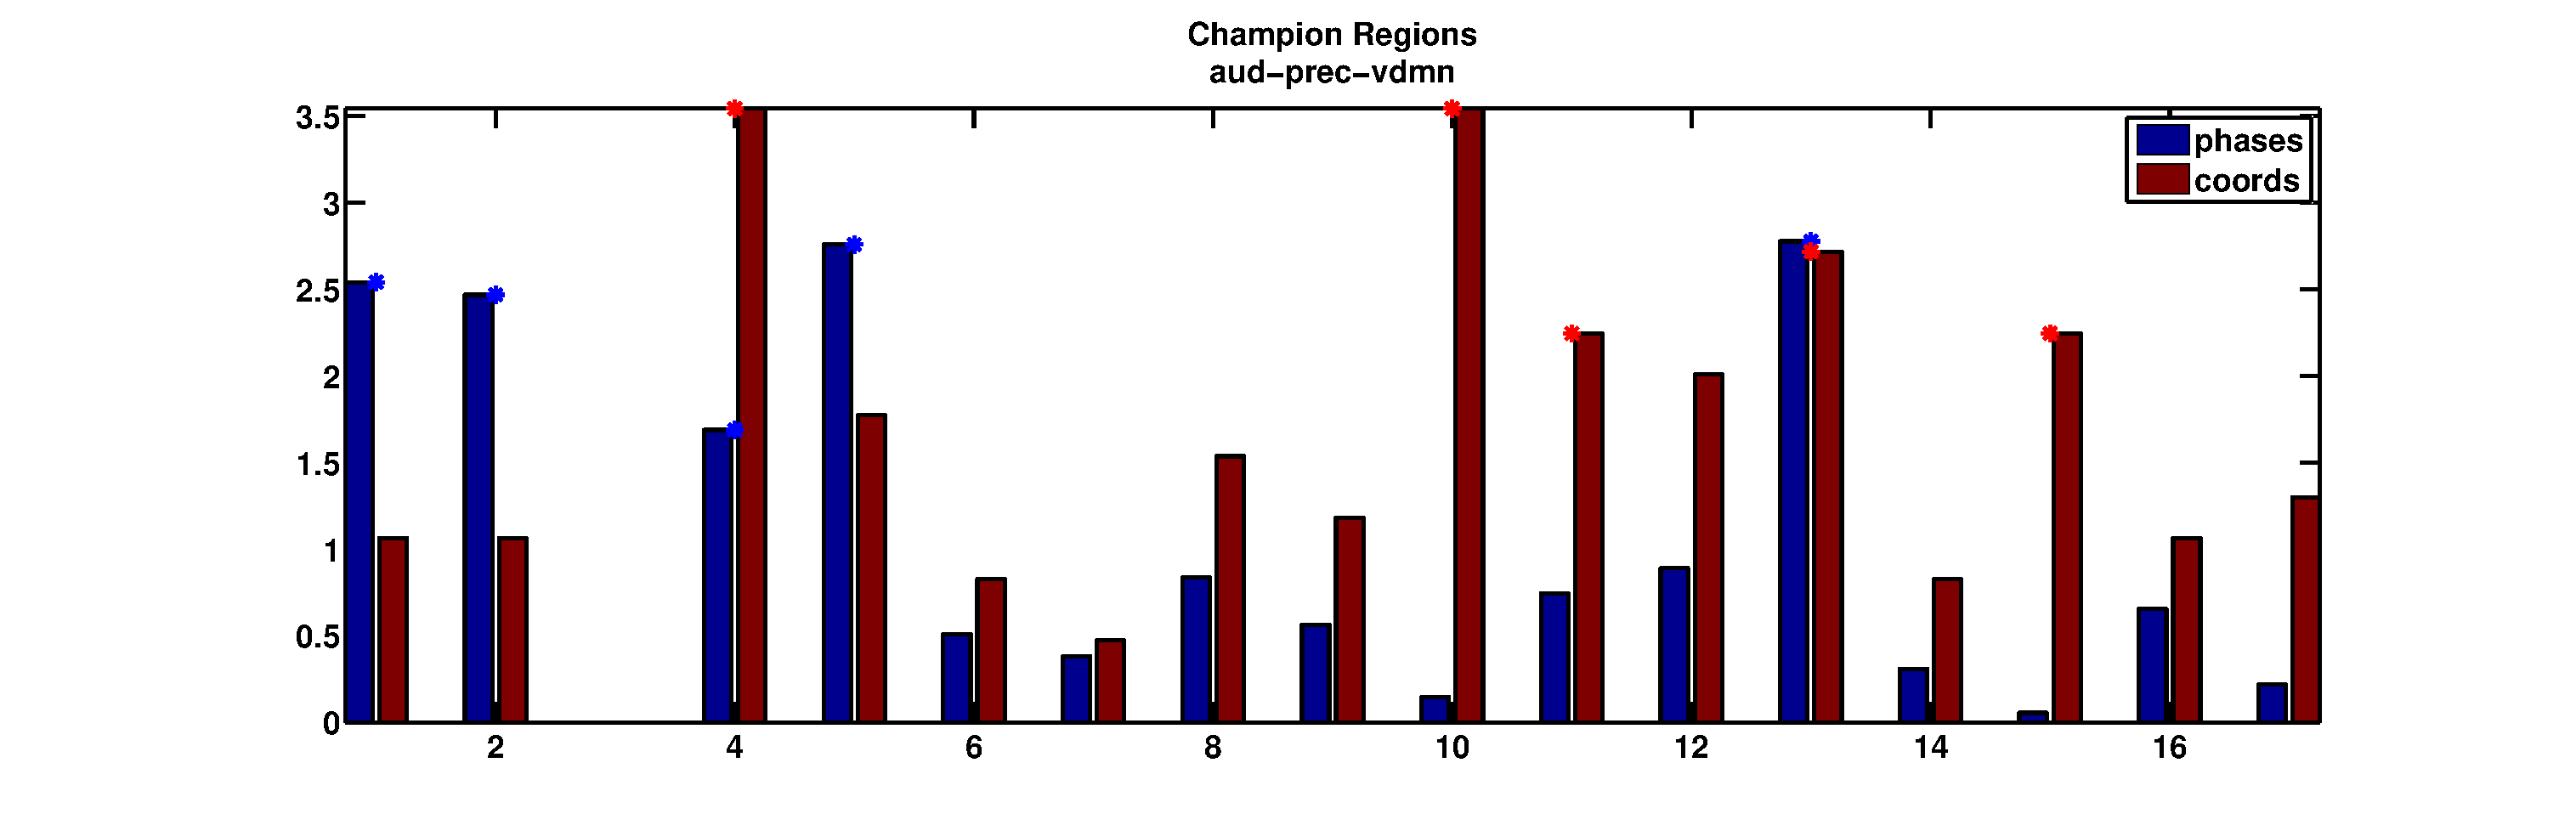
\includegraphics[trim= 150 0 130 0, clip, width = \textwidth]{pictures/hist_n5_cyclicity_aud-prec-vdmn.eps}
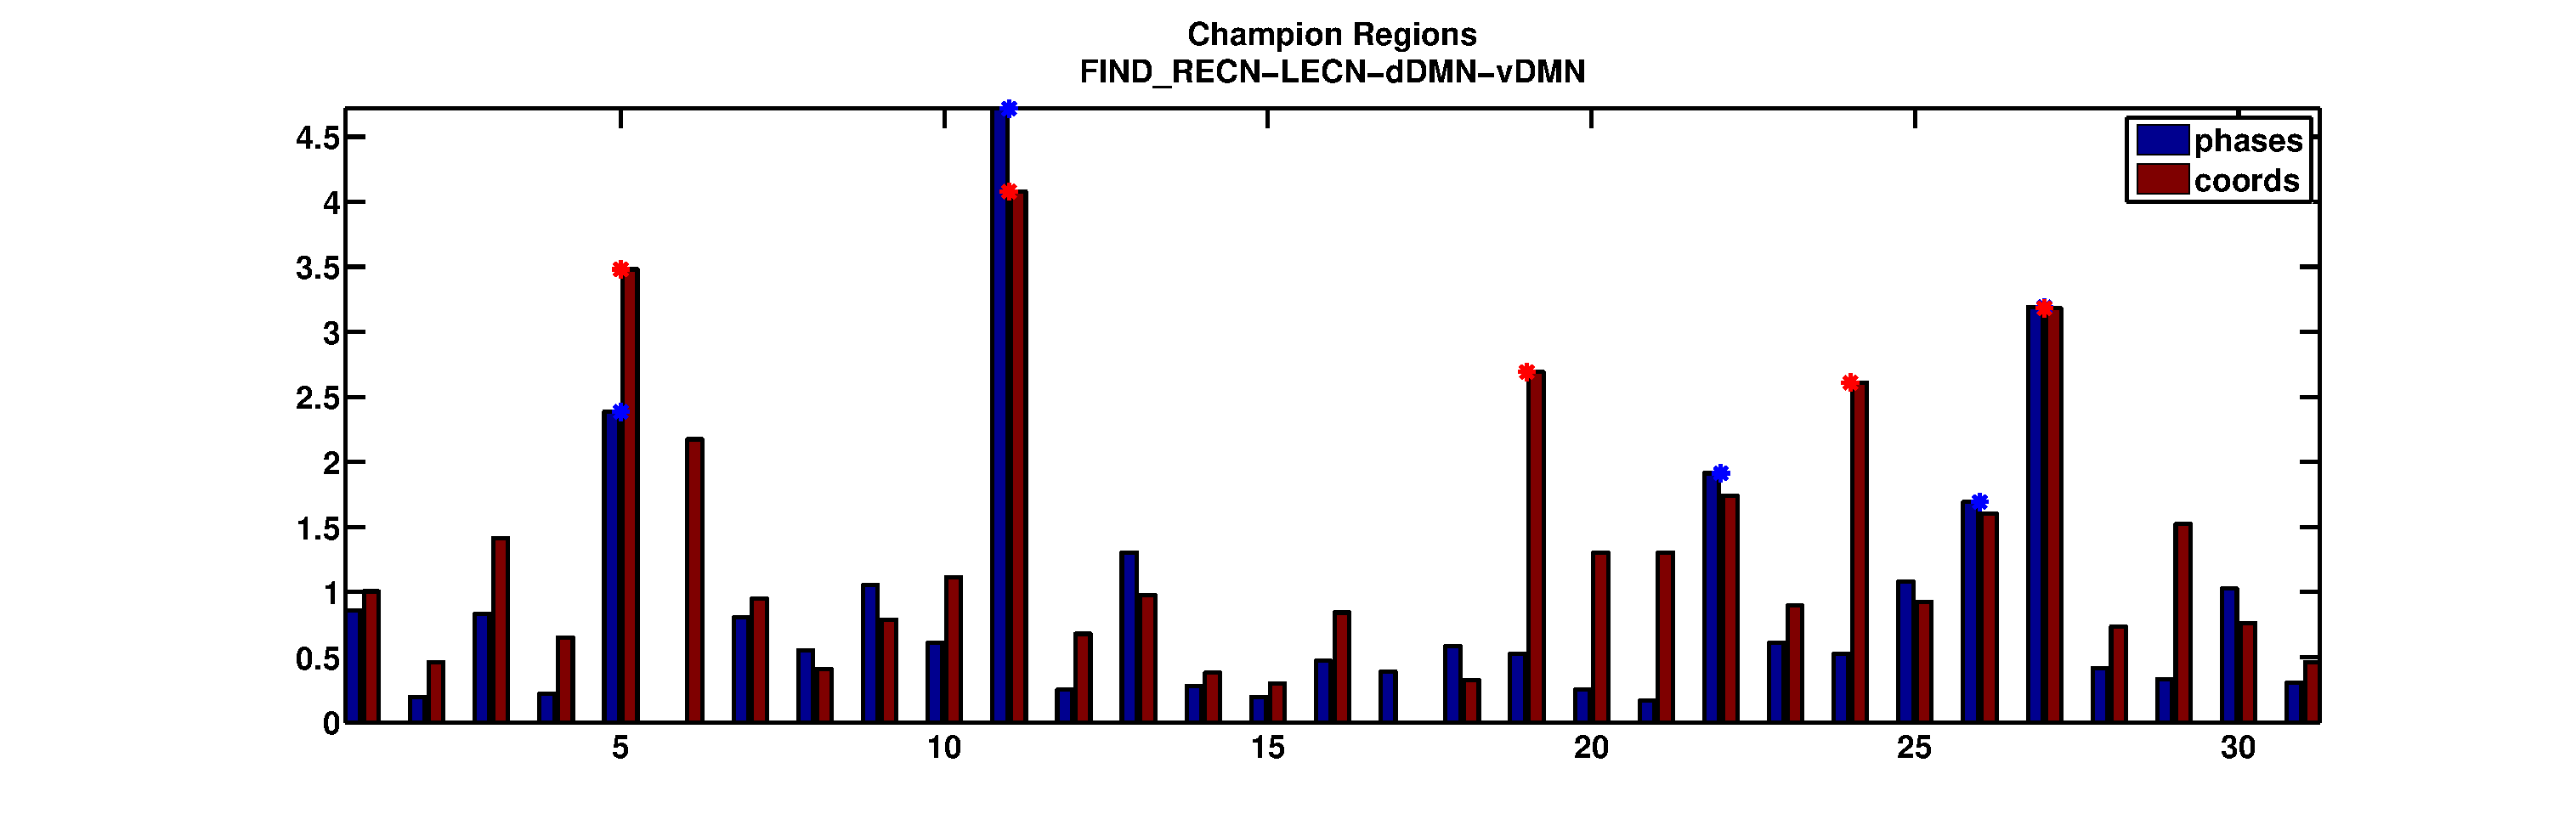
\includegraphics[trim= 150 0 130 0, clip, width = \textwidth]{pictures/hist_n5_cyclicity_FIND_RECN-LECN-dDMN-vDMN.eps}
\caption{}
\end{figure}
\begin{figure}
\label{fig:eval_ratio}
\centering
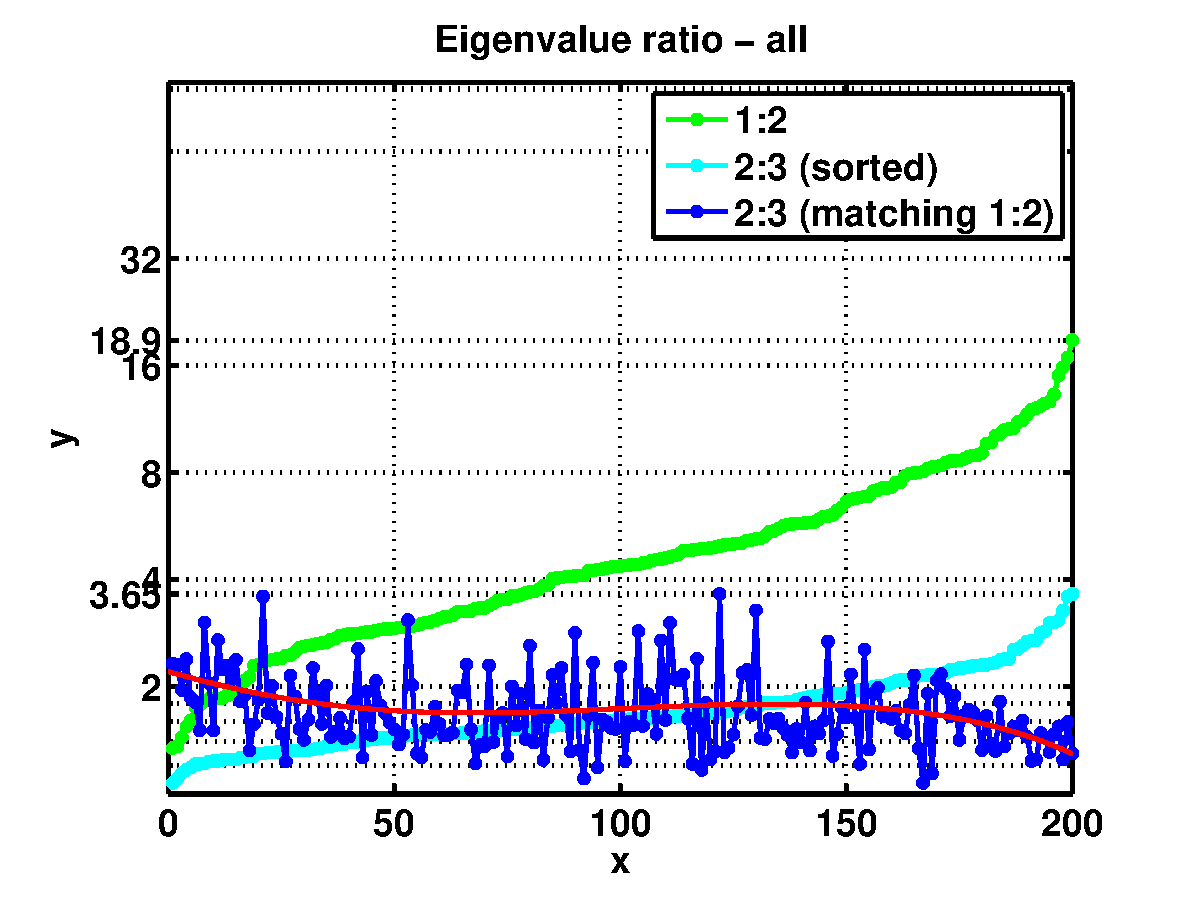
\includegraphics[width=.45\textwidth]{pictures/eval_ratio_new_FIND_all.eps}
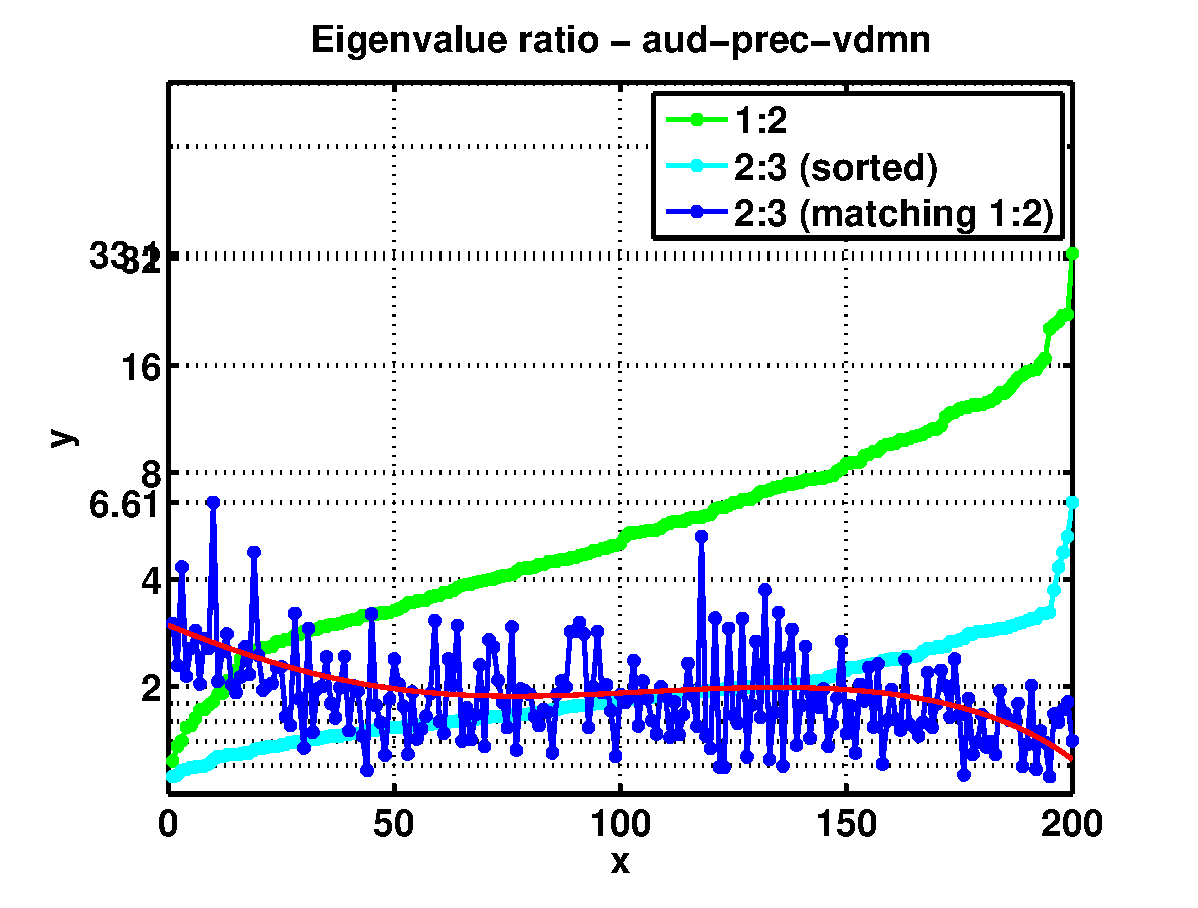
\includegraphics[width=.45\textwidth]{pictures/eval_ratio_new_aud-prec-vdmn.eps}
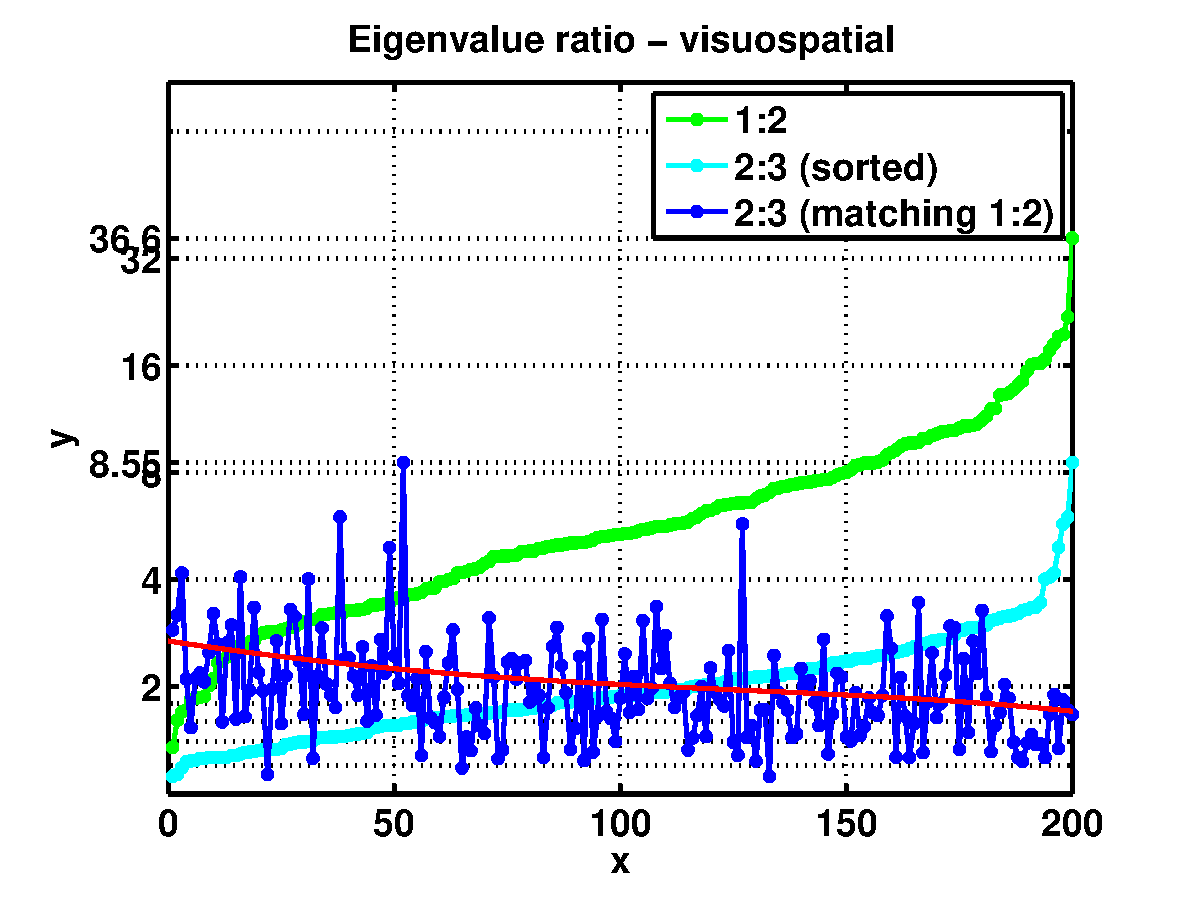
\includegraphics[width=.45\textwidth]{pictures/eval_ratio_new_FIND_Visuospatial.eps}
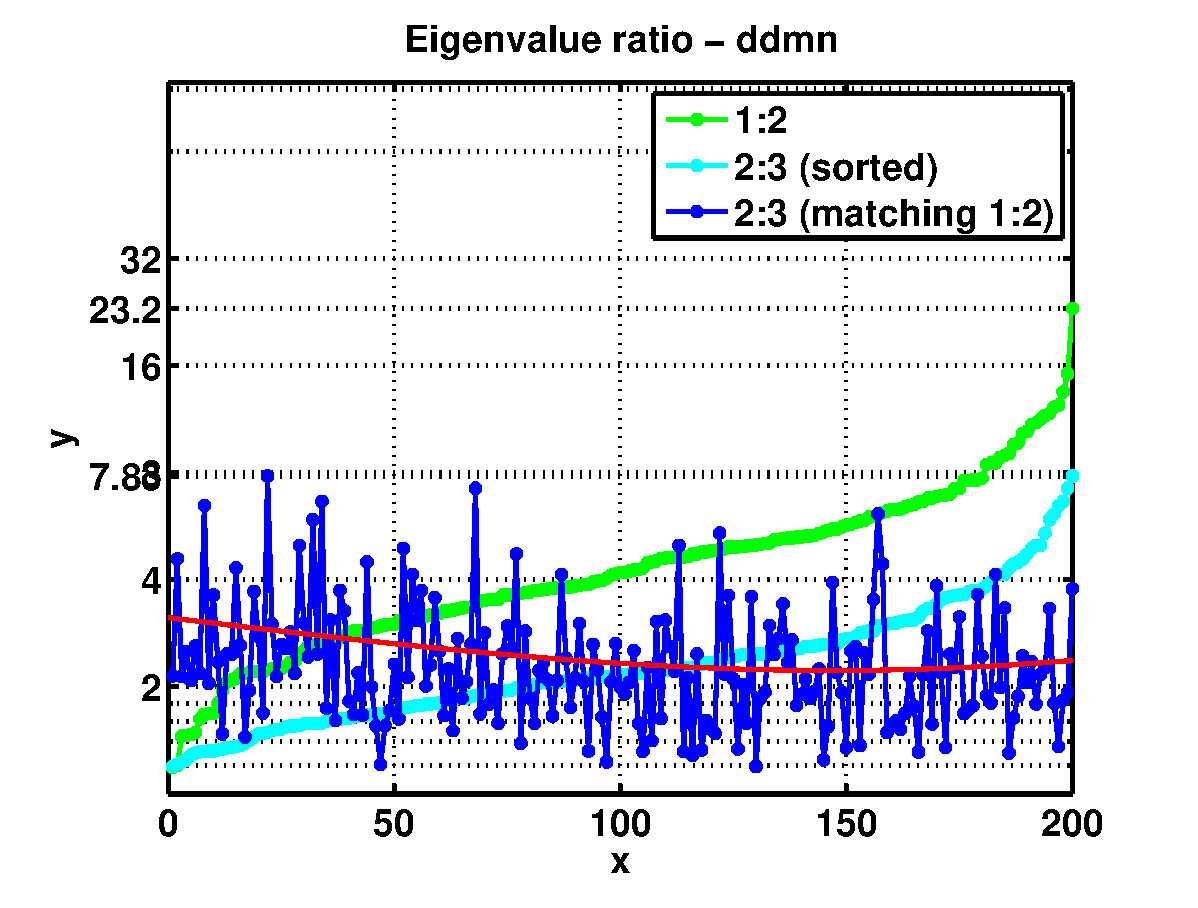
\includegraphics[width=.45\textwidth]{pictures/eval_ratio_new_FIND_dDMN.eps}
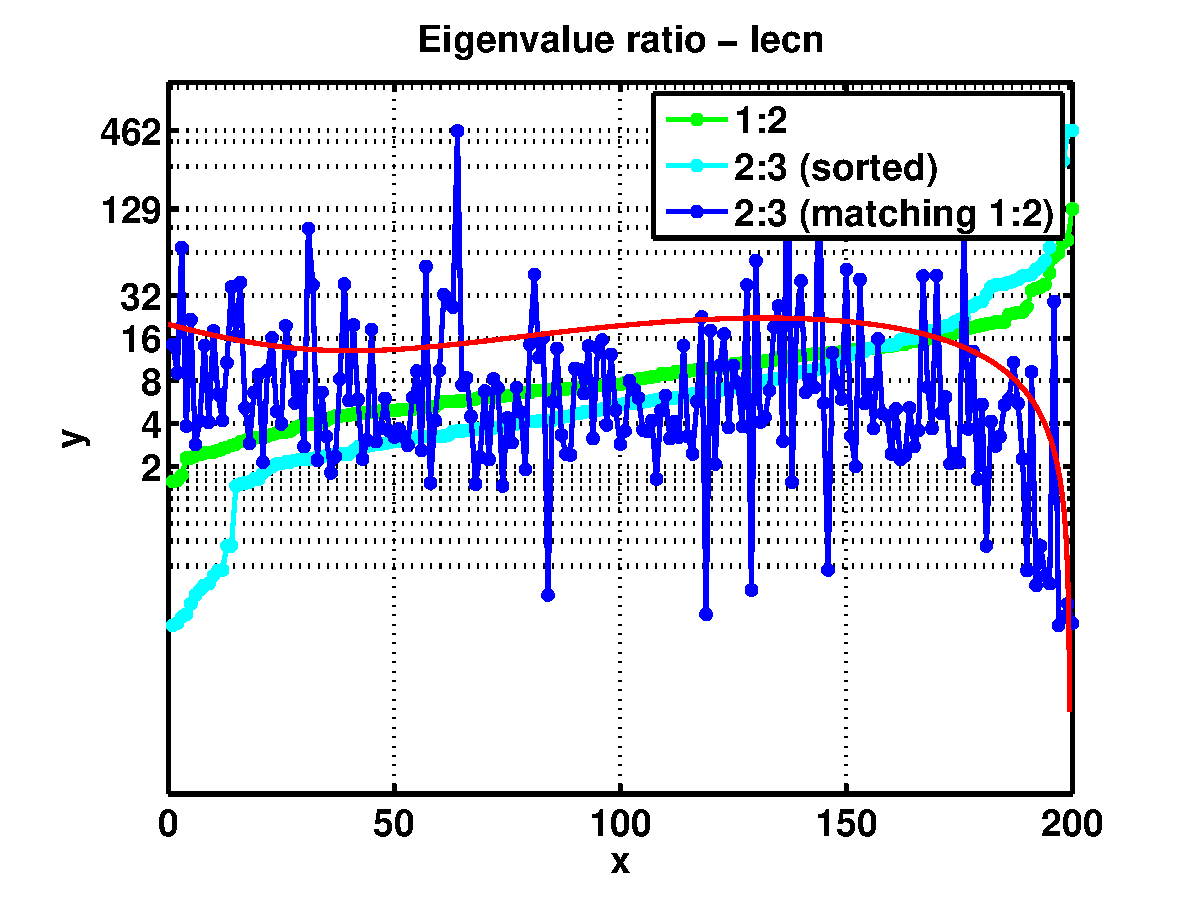
\includegraphics[width=.45\textwidth]{pictures/eval_ratio_new_FIND_LECN.eps}
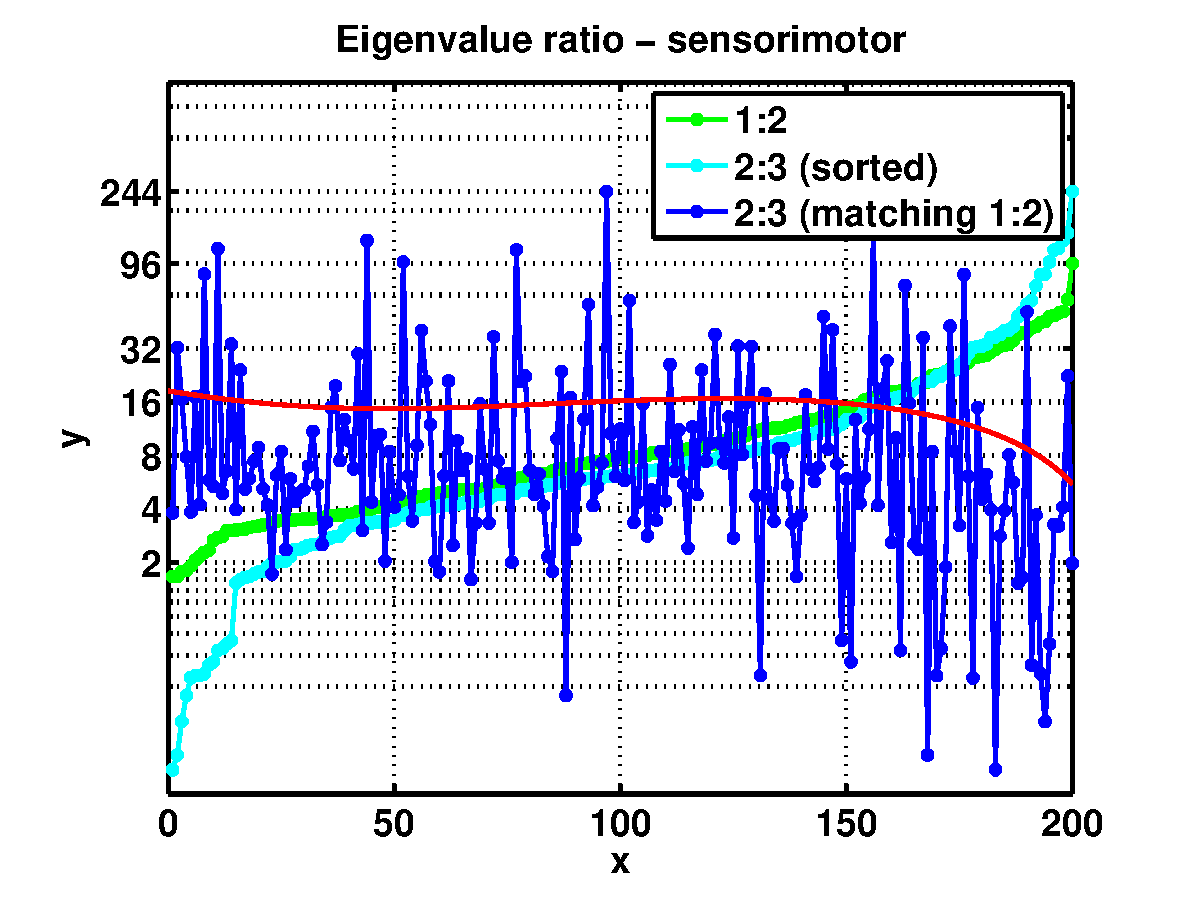
\includegraphics[width=.45\textwidth]{pictures/eval_ratio_new_FIND_sensorimotor.eps}
\caption{}
\end{figure}
\subsection{Comparison of champions: triples v. phases}
Out of curiosity, I wanted to compare the regions that show up the most in the top triples (those that are present in at least 70\% of subjects) to the regions that have the highest phase magnitudes. I was expecting the regions to more or less match up since those with higher phase magnitudes are considered more certain, but they often don't, and in some cases, a region which is very low on the phase rating, is very high in the triples rating. Note, in particular, regions 92, 10, and 6 in the first, second, and third plots, respectively, in figure (\ref{fig:hist}).

Something that may also be informative, but less surprising, is a closer look at the eigenvalue ratios. Figure (\ref{fig:eval_ratio}) shows the eigenvalue ratios for several regions or groups of regions. The top two plots show eigenvalue ratios for larger sets of regions - the plot on the left shows all regions and the plot on the right shows those in the auditory, precuneus and ventral DMN functional groups. The next row of plots shows the eigenvalue ratios for single functional groups which we would expect to be coherent in a resting state - visuospatial and dorsal DMN. The plots on the bottom row show the ratios for functional groups which we expect to be unrelated to a resting state - left executive control and sensorimotor. 

A few differences that stand out in the bottom plots are the fact that the dark blue line jumps around more, the light blue line crosses over the green, and the maximal values are much higher (greater than 200 vs. less than 50). 

The green represents the ratio of $\lambda_1:\lambda_2$ sorted in ascending order. The light blue line is the ratio $\lambda_2:\lambda_3$ (also sorted). The dark blue is $\lambda_2:\lambda_3$, but this time sorted using the ordering of the sorted $\lambda_1:\lambda_2$ trace so that the ratios can be directly compared. The red line shows a cubic fit of the blue line (other fits might be more informative... exp2 fits the ordered ratios pretty well).

\subsection{Correlations}
\begin{figure}
\label{fig:corr1}
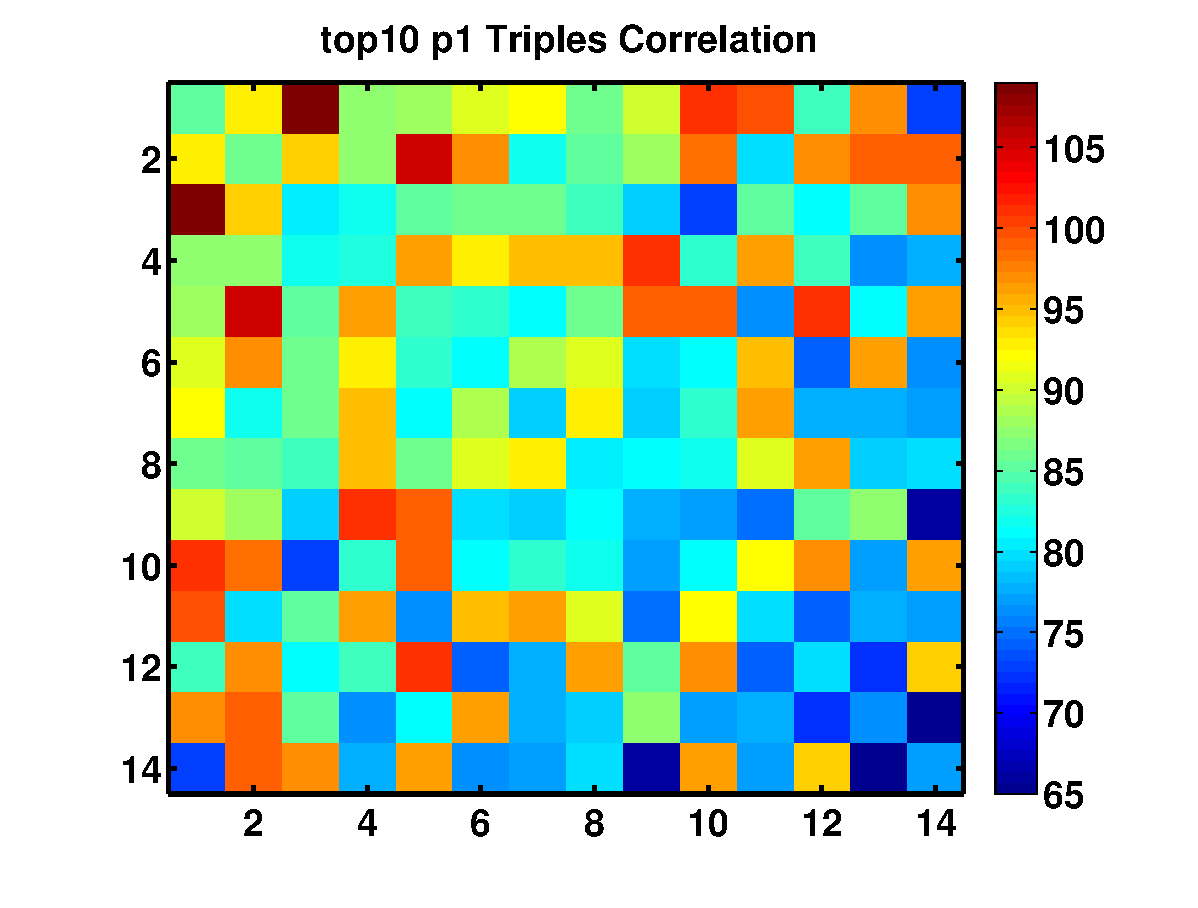
\includegraphics[width=.5\textwidth]{pictures/top10_p1_trips_corr.eps}
\begin{tabular}{|l|l|}
\hline
1&030907\\
2&010305\\
3&010907\\
4&030604\\
5&010306\\
6&030504\\
7&030804\\
8&031004\\
9&030607\\
10&010309\\
11&030904\\
12&010310\\
13&030507\\
14&010307\\
\hline
\end{tabular}
\caption{}
\end{figure}
Figure (\ref{fig:corr1}) shows the correlation between Group 1 cyclic-normalized triples. For each subject, the algorithm generates triples from the permutation and then for each triple in the set of champions, the algorithm counts which other champion triples are present and then adds one to the corresponding place in the correlation matrix. The algorithm is way too slow right now, but I wanted to make sure this is what we are trying to look at before optimizing.

\section{3/15/16}
\subsection{Regions}
\begin{table}[H]
\begin{tabular}{ll}
1 & r parahippocampus\\
2 & l parahippocampus\\
3 & medial prefrontal cortex\\
4 & posterior cingulate cortex\\
5 & precuneus\\
6 & l inferior frontal lobe\\
7 & r inferior frontal lobe\\
8 & l primary auditory cortex\\
9 & r primary auditory cortex\\
10 & l frontal eye field\\
11 & r frontal eye field\\
12 & r ventral intraparietal sulcus\\
13 & l ventral intraparietal sulcus\\
14 & r posterior intraparietal sulc\\
15 & l posterior intraparietal sulc\\
16 & l inferior parietal lobe\\
17 & r inferior partietal lobe\\
18 & r superior temporal junction\\
19 & l superior temporal junction\\
20 & r superior temporal sulcus\\
21 & l superior temporal sulcus\\
22 & r mid frontal gyrus\\
23 & l mid frontal gyrus\\
24 & r anterior insula\\
25 & l anterior insula\\
26 & r amygdala\\
27 & l amygdala\\
28 & r primary visual cortex\\
29 & l primary visual cortex\\
30 & l cuneus\\
31 & r cuneus\\
32 & r superior occipital lobe\\
33 & l superior occipital lobe\\
\end{tabular}
\caption{Regions from Fatima and Sara}
\end{table}

\subsection{Comparison of champions using scatter plots}
\begin{figure}[H]
\centering
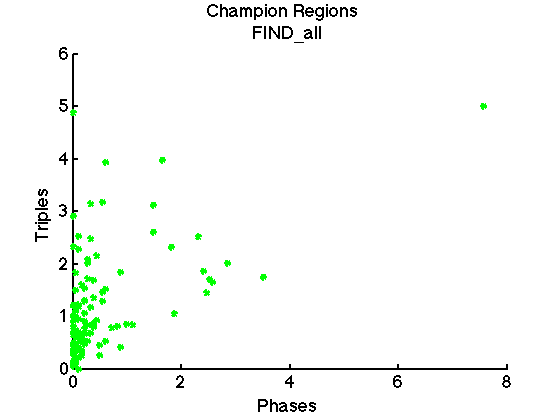
\includegraphics[width=.32\textwidth]{pictures/scatter_n5_cyclicity_FIND_all.png}
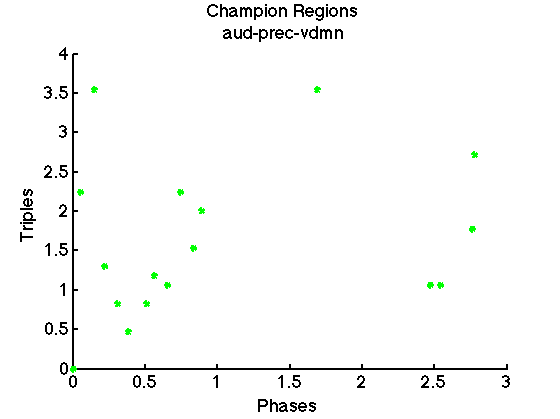
\includegraphics[width=.32\textwidth]{pictures/scatter_n5_cyclicity_aud-prec-vdmn.png}
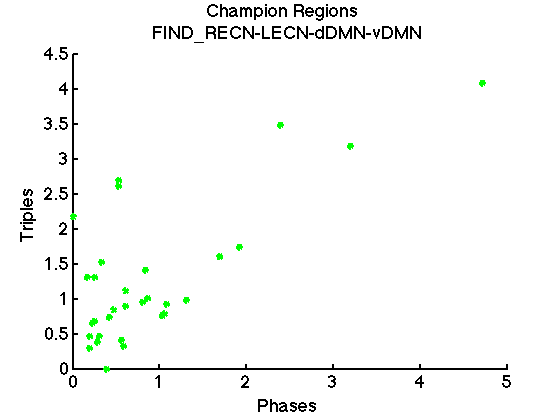
\includegraphics[width=.32\textwidth]{pictures/scatter_n5_cyclicity_FIND_RECN-LECN-dDMN-vDMN.png}
\caption{Same data as \ref{fig:hist}, but displayed as scatter plots. }
\end{figure}

\subsection{Correlations (continued)}
Recall Figure \ref{fig:corr1} shows the correlations between the triples which are present in at least 60\% of subjects from the top 10 regions (in terms of phase magnitude, phase 1). The following plots show similar analyses.
\begin{figure}[h]
\begin{minipage}{.45\textwidth}
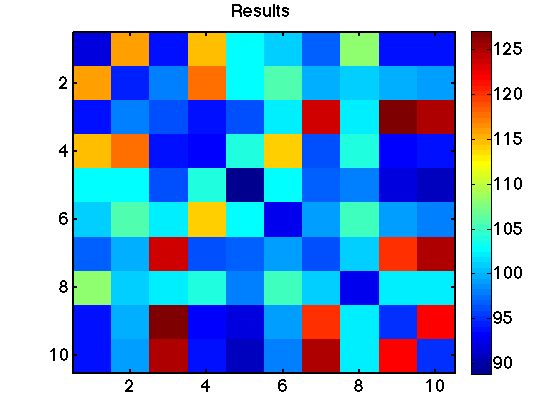
\includegraphics[width=\textwidth]{pictures/correlations_Results.png}
\vskip -10pt
\caption{Triples: present in at least 70\% of subjects. Regions: Fatima \& Sara - all}
\end{minipage}
\hfill
\begin{minipage}{.45\textwidth}
\vskip -10pt
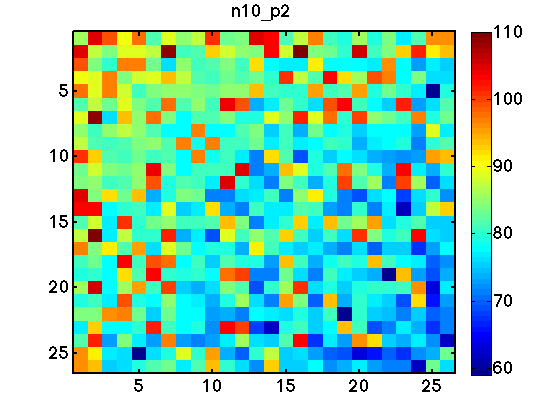
\includegraphics[width=\textwidth]{pictures/correlations_n10_p2.png}
\vskip -10pt
\caption{Triples: $\geq$ 60\%. Regions: F\&S - top 10, phase 2}
\end{minipage}
\vskip 20pt
\begin{minipage}{.45\textwidth}
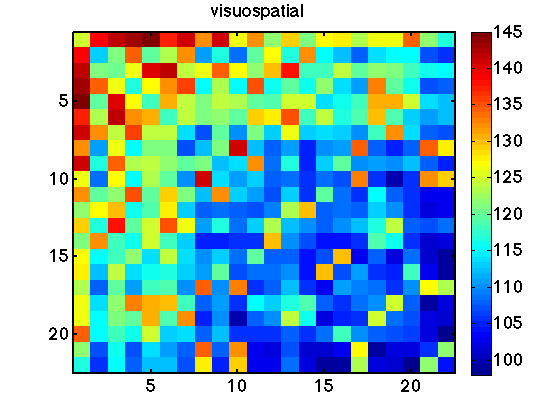
\includegraphics[width=\textwidth]{pictures/correlations_FIND-visuospatial_c70.png}
\vskip -10pt
\caption{Triples: $\geq$ 70\%. Regions: FIND - visuospatial}
\end{minipage}
\hfill
\begin{minipage}{.45\textwidth}
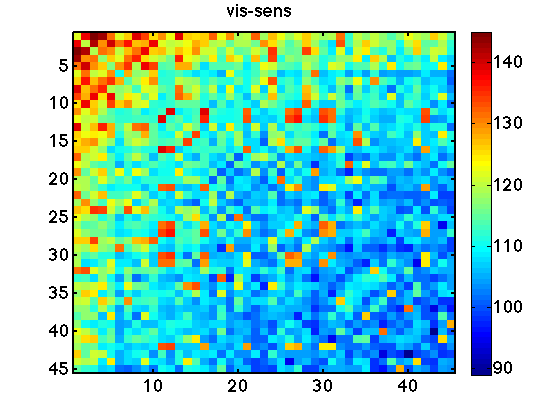
\includegraphics[width=\textwidth]{pictures/correlations_FIND-vis-sens_c70.png}
\vskip -10pt
\caption{Triples: $\geq$ 70\%. Regions: FIND - visuospatial \& sensorimotor}
\end{minipage}
\end{figure}

\section{Appendix 1: Lead matrix histograms for each (i,j) pair}
\label{app:slm_hist}
\begin{figure}[H]
\input{tex_App1}
\caption{Histograms of lead matrix values for each (i,j) pair. All histograms are on the same scale for easy comparison.}
\end{figure}
\end{document}